
\documentclass[12pt]{gatechthesis}

% -- The following packages were added by Nirbhay on June 15, 2024:
\usepackage{cleveref}
\usepackage{tabularx}
\usepackage{booktabs}
% \usepackage{xltabular}
% \usepackage{longtable}
\usepackage{incgraph,tikz}


% --------------------

% preamble

\title{Good Enough Explanations: How can local publics understand and explain Civic Predictive Systems?}
\author{Shubhangi Gupta}
\approvaldate{Jul 10, 2024}
\school{School of Literature, Media, and Communication}
\department{Department of Digital Media}
\degree{Doctor of Philosophy} 
\bibliography{references}

\newcommand{\todo}[1]{\textcolor{red}{TODO: #1}}
% document body
\begin{document}

\makeTitlePage{August}{2024}

% In \begin{approvalPage}{N}, the parameter N is the number of members in the committee. If this is less than 4, the layout of the page is single-column rather than two-column, so change the value accordingly.

\begin{approvalPage}{6}

% Add people in the following format:
% \committeeMember{Member Name}{Member Department/Position}{Member Affiliation}


\committeeMember{Dr. Yanni Loukissas, Advisor}{School of Literature, Media, and \\Communication}{Georgia Institute of Technology}

\committeeMember{Dr. Noura Howell}{School of Literature, Media, and \\Communication}{Georgia Institute of Technology}

\committeeMember{Dr. Richmond Wong}{School of Literature, Media, and \\Communication}{Georgia Institute of Technology}

\committeeMember{Dr. Chris Le Dantec}{College of Arts, Media, and Design and
Khoury College of Computer Sciences}{Northeastern University}
\\
\committeeMember{Dr. Lauren Klein}{Departments of English and Quantitative Theory \& Methods}{Emory University}



\end{approvalPage}
% \makeEpigraph{I'm not super. Any talents I have, I worked for -- it seems a long time since I thought of myself as a hero.}{Oliver Queen}
% \makeDedication{For my cousin Kara}

\begin{frontmatter}
    
\begin{acknowledgments}

I feel privileged to have been surrounded by very kind, supportive, and joyful people during the course of my PhD. They have helped me grow not just as a researcher, but as a person. Here, I want to express my heart-felt gratitude to everyone without whom this dissertation would not be possible.

To my advisor, Yanni, your confidence in my work has meant more to me than I can put in words here. Thank you for being the mentor, researcher, collaborator, and writer I aspire to be one day. You have constantly guided me, challenged me, and inspired me in critical and constructive ways. It has been an absolute honor being advised by you. 

To my committee members, Richmond, Noura, Lauren, and Chris, thank you for your support these past few years. You have been very generous with your time and have helped me develop my ideas and writings that have eventually shaped this work in fundamental ways. 

To everyone who funded me in this journey; Carol, thank you for inviting me to join the Women, Science, and Technology Learning Community, and financially supporting the entirety of my PhD, never wavering. You have been a constant calming presence in this journey that was sometimes very messy and overwhelming. And Allen, who funded my summers and supported my conference travels, thank you so much. 

To my internship mentors, Sonam, Juanis, and Sara, thank you for keeping me in touch with the world outside of academia. You all have been invaluable in helping me discover what I truly want out of my PhD. You all continue to be my mentors to this day and for that, I am so grateful. 

To my small but mighty Digital Media family, a lot of us started our grad school during COVID, unaware of what a `normal' PhD life looks like. We together created a new normal for us, a normal that I have greatly enjoyed and that I will miss so much. Pooja, Mohsin, and Sylvia thank you for constantly brainstorming with me, reviewing my writing, cheering me on, pushing me to reach for things I thought I could not achieve, and most importantly for being my friend. It would have been a very lonely journey if it weren't for you all. 

To all other friends within and beyond Georgia Tech, Kiran, Jaya, Nikhil, Sushant, Aditya, Vishal, Manoj, Atefeh, Vaibhav, and so so many more people who I may not be able to name here, thank you for listening to my many many rants, for  helping me disconnect from work when needed, and for making sure I enjoy this journey. 

To my fiancé, Nirbhay, you challenged me to start this journey and held my hand as I completed it. Intellectually, you have been my sounding board, my fresh eyes, who has helped me develop each and every argument I make in this work. Emotionally, you have been my rock, who has kept me in touch with who I want to be and what I want to do in this fleeting life. This journey wouldn't be nearly as exciting or gratifying if it weren't for you.  

And lastly, my family, my parents Prabha and Puneet, my brother Manush, and my sister (in law) Priyanshi; Mom and Dad, the list of things I should thank you for is endless. You have shown me what it means to live a wholesome life, a happy life, a life full of love and laughter. It is a privilege to be your daughter. I owe it all to you both. Manush, my big brother, whose footsteps I first followed but who helped me become my own person in time. Thank you for being there for me in times that truly mattered. And Priyanshi, my new sister, thank you for joining our family and ending my PhD journey on a high! 

Mentors, friends, and family, I will cherish my memories with you all forever. Thank you for everything! 


\end{acknowledgments}

    \makeTOC
    \makeListOfTables
    \makeListOfFigures
    \input{abbrevs}
    
\begin{summary}

\emph{How can the Explainable Artificial Intelligence (XAI) community support public understanding of the spatial workings and effects of civic predictive systems?} Civic processes in the urban smart city are increasingly being governed by automated predictive systems using machine learning models. Despite their widespread use in everyday domains such as education, policing, social services, and economic investments, they continue to remain invisible and inaccessible to local publics, who bear the burden of their effects. XAI and Artificial Intelligence (AI) transparency researchers are increasingly calling for the development of public-centered AI explanations. However, in the context of civic AI, existing techniques fall short in (1) how they understand the consumers and creators of explanations, (2) how they explain the socio-technical assemblages that give rise to AI systems,  (3) how they design interactions to create and deliver explanations, and (4) how they conceptualize explanation goals in relation to public action. This dissertation engages in qualitative, participatory, and design-based research to introduce the concept of `good enough explanations' in response to these challenges. Good enough explanations may not be complete or universal. Instead, as this dissertation formulates, such explanations consist of \emph{ongoing processes} that allow \emph{diverse publics} to \textit{partially} engage with \emph{features of predictive systems} and \emph{assess such systems in relation to their communities}.  This dissertation (1) theorizes qualities underlying good enough explanations, (2) engages in the development of such explanations with diverse publics, and (3) suggests theories and strategies to guide the development of systems for good enough explaining. 

Ultimately, this dissertation hopes to serve as a guide for XAI researchers, civic organizations, as well as policymakers, as they work together to engage with publics for the democratic oversight, assessment, and regulation of civic AI systems. 


\end{summary}
\end{frontmatter}

\begin{thesisbody}
    \chapter{Introduction} \label{ch1:intro}
\emph{How can the Explainable AI (XAI) community support public understanding of the spatial workings and effects of civic predictive systems?} 

Civic predictive systems, or systems that affect civic processes, are becoming an inseparable part of the urban smart city.  They inform several fundamental decisions that govern our everyday lives: who gets parole, bail \cite{arnold}, or economic and social aid \cite{noriega2020algorithmic}; who gets hired \cite{raghavan2020mitigating}; how are students assigned to public schools \cite{robertson2021modeling}; how well are teachers performing \cite{teachereval}; which child welfare calls need immediate attention \cite{chouldechova2018case, cheng2021soliciting}; how un-housed people receive housing resources \cite{kuo2023understanding}; who gets a loan application approved \cite{schoeffer2022there}; or which routes we, or our public transports, take in a city \cite{gupta2022rethinking, goodman2019challenge}. They are pervasive. 

The use of predictive systems has been presented as making civic processes more efficient, accurate, and objective. They can effectively and quickly process large amounts of data about a variety of subjects and their environments.  They can identify patterns not previously known while attempting to overcome biases in human-based decision-making \cite{brauneis2018algorithmic}. The hope is that the use of such systems can address the resource constraints within the public sector by off-handing or automating labor, thereby reducing costs and increasing resource allocation capacities \cite{levy2021algorithms}. 

Despite their proposed vision and goals, several civic predictive systems have been shown to cause societal harm and discrimination \cite{eubanks2018automating}. There are countless examples of bias \cite{bartlett2022consumer, dastin2022amazon}, disregard of civil rights and liberties \cite{de2020states, johnson2023face}, or privacy invasions \cite{ice}. The centralized and authoritative nature of algorithms gives them the power to create or reinforce unjust (and often invisible) societal structures and inequalities \cite{d2020data}.  

Geospatial civic algorithms specifically, that make predictions about spaces in the smart city, attempt to fit highly complex cities into neat structures demanded for computation \cite{mattern2020city}. Critical geographers, such as Schwanenand and Kwan, demonstrate how social discrimination and marginalization are inherently entangled with space \cite{kwan2012critical}. The overly simplistic mathematical representation of cities creates the kinds of invisible inequalities and incremental injustices that produce large-scale societal effects, such as gentrification and segregation \cite{loukissas2022wants}. Numerous cases exemplify the inequitable spatial effects on diverse communities:

\leftskip 20pt
\rightskip 0pt plus 1fill
\vspace{8pt}

Planning algorithms such as the Market Value Analysis present governing bodies with a “data-driven objective” means of distributing public resources by classifying and segregating communities through the construction of color-coded boundaries. Such organization of space, as Safransky argues, standardizes unjust classification systems and restructures the public sphere in ways that favor some neighborhoods over others. These civic algorithms are opaque, inaccessible, and are rarely if ever, developed through a public and participatory process \cite{safransky2020geographies}.

Sociologists such as Zukin et al. have demonstrated how geographically coded Yelp reviews reinforce prejudice against neighborhoods with people of color thereby influencing civic investments and contributing to processes of urban change such as gentrification. The algorithmic moderation of reviews is not public, and users are unaware of their role in affecting capital flows \cite{zukin2017omnivore}.

Loukissas argues that filter bubbles created by Zillow reinforce existing spatial power structures along the axes of race and class. Even as the goal of the site is to give users more control over their home-buying experience, it leaves users unaware of the implications of their own filtering decisions \cite{loukissas2022wants}.

In my past work, I illustrate how safe walking apps, such as Safetipin, risk segregating neighborhoods by attempting to advance the safety of one social group while marginalizing another. Once again, knowledge about the failings of social structures and policy normalized by the app is inaccessible to citizens, as well as the app creators \cite{gupta2022rethinking}.

\leftskip 0pt
\rightskip 0pt 
\vspace{8pt}

Without careful consideration of the spatial workings and effects of predictive systems, they risk reproducing or even amplifying historical systems of discrimination. Currently, civic algorithms are deployed in ways that prevent citizens from getting access to them or learning about their existence and effects. This limits the citizens' ability  to contest, oversee, assess, or protest automated decisions that affect their lives in fundamental ways. To address concerns of algorithmic opaqueness and lack of understanding, activists \cite{stop_lapd}, civic organizations \cite{lee2023making,post}, as well as several governmental agencies \cite{white2022blueprint} are calling for advancements in algorithmic transparency, explainability, and impact assessment.  Their goal is to drive visibility into the design of algorithms, opening them up for critique and evaluation by both experts and everyday users.  

\section{Existing XAI and AI Transparency Approaches}

Early research on Explainable AI focused majorly on technical explainablity and transparency. For black-boxed algorithms, post-hoc explanations where another human-interpretable model imitates the practices of a complex model are being designed to understand how an algorithm makes its predictions. Guidotti et al. \cite{guidotti2018survey} categorize post-hoc explanations into these categories: (1) Global Model Explanations where a simpler interpretable model is trained on the same data to approximate the working of the primary more complex model, (2) Outcome Explanations where the focus is on explaining one outcome or instance of prediction by providing the weight of features that contributed to it \cite{schuff2022human} or examples of inputs that would lead to a similar prediction, and (3) Counterfactual Explanations where the goal is to identify what should be changed in the inputs to get a different prediction \cite{shang2022not}. Beyond making models interpretable, XAI efforts attempt to make known other aspects of the machine learning model such as datasets, training algorithms, source code, and performance metrics \cite{vaughan2020human}. Several model \cite{mitchell2019model} and data documentation \cite{anik2021data, bender2018data, gebru2021datasheets, holland2020dataset} frameworks, have been designed to explain AI to experts \cite{dhanorkar2021needs}. Frameworks such as `CrowdWorkSheets' support standardized documentation of decisions when annotating datasets in a crowdsourced manner \cite{diaz2022crowdworksheets}. `Data Cards' provide summaries of datasets for various stakeholders \cite{pushkarna2022data}. To promote transparency of models, existing work proposes tools such as `Model Cards' that aim to provide details about a model related to its working, use cases, and evaluation \cite{mitchell2019model} and `Factsheets' that provide an overview of facts about specific models across the AI lifecycle \cite{richards2021human}. There is also growing work in designing open-source toolkits to identify and assess algorithmic harms and biases \cite{bellamy2018ai, wexler2019if, bird2020fairlearn}. AI Fairness 360 (AIF360) \cite{bellamy2018ai} and Fairlearn \cite{bird2020fairlearn} are tools that aim to help practitioners understand `bias' metrics and allow them to detect algorithmic biases. These tools also help mitigate said biases by providing a variety of mitigation algorithms. Another tool called ``What-If'' uses visualizations to help users and practitioners investigate how a model will perform in hypothetical scenarios created by changes in data points \cite{wexler2019if}.

More recently, the XAI community has presented the need to make AI processes visible to the general public in order to build trust in the artificially intelligent systems that guide their lives \cite{knowles2021sanction}. There has been a growth in work that focuses on developing methods and frameworks for user-centered algorithmic explanations \cite{miller2019explanation, shneiderman2020human, vaughan2020human}. Human cognitive abilities \cite{wang2019designing}, users' explanatory needs \cite{liao2020questioning, springer2020progressive}, users' situated real-world experiences \cite{devos2022toward}, users' ability to collaborate and form counter publics \cite{shen2021everyday} have been some of the guiding factors in advancing user-centered XAI research.    

Such efforts have built on diverse theories and methods: interactive explainability methods \cite{cheng2019explaining}, such as Interactive Model Cards \cite{crisan2022interactive}, have been proposed, theories describing human cognition patterns have been employed \cite{wang2019designing}, and example-based methods where data samples that informed a prediction are shown to users have been presented as helpful \cite{cai2019effects}. Additionally, several toolkits have been designed to promote user understanding of AI systems such as: TILT (transparency information language and toolkit) that organizes the information that transparency policies demand in structured ways for machines to read and users to consume \cite{grunewald2021tilt}, or AIX360 toolkit \cite{arya2019one} that present visualizations and explanation algorithms respectively to help users understand how predictive systems work. Investigations into how XAI can support user assessment \cite{robertson2022understanding} and decision-making capabilities \cite{kulesza2013too} are also being conducted.

These efforts have made monumental progress in the field of Explainable AI. Yet, there remain limits. First, they are not pluralistic in nature \cite{hancox2021epistemic, ehsan2022social} and do not consider the values, surrounding social systems, existing knowledges, and beliefs \cite{kaur2022sensible} of users in the design of explanations. Second, they may focus merely on technical transparency, disregarding the systemic factors surrounding any algorithmic decision \cite{ehsan2021expanding}. Third, they tend to be one-time explanations that portray users as passive individual consumers \cite{corbett2023interrogating}. And lastly, the goal of most explanations is to increase user trust rather than to promote critical thinking or action \cite{danry2023don}.  This leaves little room for democratically evaluating how the complex world we live in is simplified to be represented in the design of algorithms— who is included, who is excluded, and how cities are quantified and aggregated for computation. I discuss these limits in more detail in \ref{ch2:gee}. 

This dissertation aims to address these limits and theorize the design of effective public explanations of civic AI tools. I want to note that in using the term `explanations', I am not referring to the technical explanations provided through the use of algorithmic interpretability methods. Rather, I am attempting to expand our community’s understanding of `explanations' such that it is not limited to the technical understanding of the systems but is explaining the social, political, and economic development, use, and effects of civic predictive systems. 

I ground my work in public safety AI systems. Specifically, I employ place-based predictive policing as a case study for this research.


\section{Public Safety Algorithms and Harms }  

My research for this dissertation started with a critical analysis of a renowned safe walking app, primarily deployed in India, called `Safetipin' \cite{safetipin}. Safetipin recommends `safe' paths to users from an origin to a destination by calculating `safety scores' for various paths. These safety scores are calculated by aggregating crowdsourced `safety data' such as the amount of lighting, or presence of security officers, in various locations in a city. To study this tool, (1) I draw on feminist criticisms of safety technologies, defined broadly, to identify the main issues in their framing and efficacy, and (2) I build upon initial interviews with users and makers of Safetipin to examine how the app addresses, or fails to address, the criticisms received by other safety technologies.

This critical analysis demonstrates Safetipin’s capacity to (1) restrict women’s movement to computationally calculated `safe' neighborhoods and (2) reinforce caste and religion-based segregation in India \cite{gupta2022rethinking}. By disregarding the prejudice about vulnerable neighborhoods that governs the `feeling of safety' of its users who contribute to the crowdsourced data, Safetipin fails to situate itself in the broader historical politics of safety in the city \cite{kern2021feminist} that continue to marginalize people of lower socioeconomic status and minority religions. Nonetheless, the app and its underlying information infrastructures that promote segregation, have been enthusiastically accepted and celebrated \cite{safetipin_award1, safetipin_award2}. This work presents a dire need to identify and understand the impact of spatially distributed data inputs and aggregations on the city and its people. Ultimately, it motivates the need to explain how emerging civic geospatial technologies, especially in the realm of public safety, organize cities and their impact on spatial segregation and discrimination. 

Amongst other tools for public safety exist a variety of ML algorithms that have been developed with the hope to mitigate crime and advance citizen safety in smart cities. Popular examples include— COMPAS \cite{compas}, which predicts recidivism risk for an individual; Predpol (now Geolitica) \cite{predpolbad}, which predicts geographic areas where crime is most likely to happen; Arnold Public Safety Assessment \cite{demichele2020public}, which provides judges with sentencing recommendations. These algorithms, even as they aim to promote public safety in cities, tend to reinforce discrimination along the axes of race and class. Jefferson demonstrates how Predpol legitimizes the bias embedded in official crime datasets and has resulted in the over-policing of already heavily surveilled neighborhoods \cite{jefferson2018predictable}. Risk assessment tools build upon and reinforce the racist policies and infrastructures underlying carceral systems in the US. Additionally, they define `risk' at the level of an individual, disregarding how `risk' is a reflection of societal prejudice against various social groups \cite{green2020false}. In India, centralized systems and norms along with the subjectivities of individual police officers lead to historical, representational, and measurement bias in recorded crime data for the Crime Mapping Analytics and Predictive System (CMAPS) predictive policing tool. Further, the opaque design of CMAPS allows for discrimination against immigrant colonies and minority settlements by promoting the belief that crime rises in specific neighborhoods by virtue of the above-mentioned communities living there  \cite{marda2020data}. Transparency is a much-needed feature for the effective assessment and development of public safety algorithms \cite{rudin2020age}. Given the limited potential of techniques designed to “de-bias” public safety algorithms, there is an urgent need to make the data assemblages \cite{kitchin2014towards} surrounding public safety algorithms transparent and accessible to city residents and governmental bodies \cite{marda2020data}.   

This dissertation aims to study the concept of effective public explanations,  by specifically focusing on place-based predictive policing as a case study. Place-based predictive policing is a method that aims to support the efficient distribution of police resources in a city. Typically, the method utilizes historic crime data such as arrest reports or calls for service requests integrated with other social and environmental data to predict the location and time of future crimes. A popular example of such a system is called Geolitica (previously Prepdol) \cite{predpolbuy}. In the past decade, academics and activists have heavily scrutinized the use of predictive policing \cite{o2017weapons}. The tool has been shown to reproduce existing geographic and social biases embedded in historically discriminatory crime data \cite{jefferson2018predictable,akpinar2021effect}. A recent study conducted by the Markup has found the accuracy of this tool to be less than half a percent \cite{predpolbad}. Many others have discussed the incompleteness of data \cite{kirkpatrick2017s}, the inability to validate results \cite{demortain2017evaluating}, and the proliferation of positive feedback loops \cite{o2017weapons}. Such thorough investigation of this predictive tool makes it an ideal case to ground our discussions of effective public explanations. 



\section{Research Questions and Chapter Outline}

In this dissertation, I ask: \emph{How can the XAI community support public understanding of the spatial workings and effects of civic predictive systems (RQ)?} To investigate this question, I primarily employ community-centered qualitative and participatory methods. Additionally, I build on and am in conversation with scholarship from fields such as human-computer interaction (HCI) that investigates how users perceive, relate to, and interact with AI systems to seek AI explanations; science and technology studies (STS) that shines light on the socio-technical environments surrounding AI, publics affected by AI, as well as the processes of explaining and knowing; and AI Transparency and Explainability (XAI) that has designed numerous methods, frameworks, and tools to explain AI systems to a variety of audiences. 

\Cref{ch2:gee} begins my investigation of the primary research question guiding this dissertation (RQ) by asking: \emph{ What qualities underlie effective public explanations of civic predictive systems (RQ1)?} My inquiry is driven by a semi-structured interview study along with an extensive review of existing scholarship on public explanations for civic predictive systems. I interview 23 participants including academics, AI activists, journalists, community and neighborhood leaders, and civic society organizations who think, write, or act on issues of social justice and AI safety, to identify the qualities and characteristics underlying meaningful public explanations of civic predictive systems. Drawing on my findings, I introduce the concept of \emph{ ‘good enough explanations’}. ‘Good enough explanations’ as understood by our participants, (1) are \textit{situated} in the lives of diverse publics, (2) explain the complex and entangled socio-technical \textit{systems} that predictive tools interact with, (3) involve \textit{continuous and partial} processes, and lastly (4) empower publics to \textit{act} in ways that promote democratic deployment and regulation of predictive tools. Such explanations, I argue, may not be complete or objective but are good enough to support publics in critically engaging with the workings and effects of civic predictive systems in service of their goals. The rest of the dissertation attempts to understand and explore these qualities.  

\Cref{ch3:methods} documents my approach to study, as well as create, good enough explanations. \textit{Form} has been considered an essential dimension of AI Explanations \cite{van2021effect}. As such, I take inspiration from the visual history of city representation to demonstrate how \textit{mapping} may allow us to explain geo-spatial AI systems in ways that are accessible, culturally reflexive, situated, and provide visibility into how algorithms represent cities. I employ a `research through design' methodology and conduct participatory mapping workshops with diverse publics such as— police reform groups, city planners, neighborhood and community leaders, civic development agency, and educators— to investigate how can we, as XAI researchers, design good enough explanations. The workshops encouraged participants to question, understand, and explain place-based predictive policing on their own terms by using maps to ground discussions in the spaces they live and work in. The explanation contexts that emerged were analyzed using inductive coding, situational analysis, memo-ing, and thematic analysis. These workshops support the findings and arguments developed in chapters 4, 5, and 6.

\Cref{ch4:situated} studies the `situated' nature of public explanations and asks: \emph{How are explanations situated in the lives of diverse publics and what does that mean for the design of public explanations (RQ2)?} Drawing on five participatory mapping workshops with diverse publics, this chapter reflects on the explanation contexts that emerge when publics question or understand AI systems. I find that when attempting to understand AI systems, publics draw on their relation with not just the predictive technology, but also the prediction domain, prediction subject, and prediction backdrops. Situated explanation needs of publics emerge out of these entangled relations. I argue that these broader relations play a significant role in supporting public understanding of civic AI systems and urge XAI researchers to consider these relations as they attempt to design systems for public understanding of AI. 

Chapter 5 studies the `systemic' nature of public explanations and asks: \emph{How can the XAI community help explain the complex socio-technical systems that civic AI tools engage with?} Underlying AI systems are socio-technical assemblages of materials, relations, cultures, institutions, and histories. In this chapter, I analyse the participatory mapping workshops using situational analysis to demonstrate the ability of local publics to partially explain the environments AI tools are deployed in, the cultures and norms they invade, and the lived experiences of the problems they attempt to address. Drawing on these findings, I argue that good enough explanations need not be designed in isolation \emph{for} publics \emph{by} XAI researchers. Instead, XAI researchers would benefit from co-creating systemic explanations \emph{with} diverse local publics through slow and long-lasting engagements.  

Chapter 6 reflects on the methods I use to develop good enough explanations to reconceptualize explanations as explain\emph{ing}— a continuous and partial process that supports the development of \emph{situated} understandings of AI \emph{systems}. I provide a detailed account of three design dimensions I believe should be considered as XAI researchers design spaces and systems that mediate processes of explaining: (1) designing explaining sites (2) designing explaining media, and (3) designing explaining interactions. I briefly discuss how explain\textit{ing} may influence public `action'. I end by providing a list of questions that XAI researchers can consider as they attempt to create good enough explanations for civic predictive systems.  

Lastly, I conclude by providing a summary of the research conducted in this dissertation, highlighting limits of this work, proposing relevant future work, and positioning the work in relation to my background and motivations. 

Together, these chapters attempt to make three primary contributions to the field of XAI: (1) theoretical contribution by conceptualizing what \emph{good enough explanations} mean for public understanding of civic predictive systems, (2) empirical contribution by reporting how diverse publics may understand, question, and explain civic predictive systems, and (3) methodological contribution by demonstrating and recommending strategies for co-creating a good enough understanding of civic predictive systems.  

My hope is that this work will support XAI researchers, policymakers, and community leaders in designing systems and spaces for public engagement with civic predictive systems. Such engagements, as stated in \Cref{ch2:gee}, should work to promote democratic public action toward contesting, redesigning, regulating, or discontinuing predictive systems that may cause societal harm in fundamental yet currently invisible ways.  

   
    % 
\chapter{Background}

\subsection{Exiting methods to explain AI systems as socio-technical assemblages}

Majority of existing efforts to explain AI focus on technical components such as algorithmic features and their weights, training datasets, source code, and performance metrics \cite{vaughan2021human}. Recently, the XAI community has called for moving beyond technical transparency and considering other socio-technical elements impacting AI decision-making. Few but growing frameworks and concepts are being proposed. Ehsan et al. introduce social transparency, which includes making transparent the technological context, decision-making context, and organizational context surrounding algorithms \cite{ehsan2021expanding}. Similarly, Kroeger et al. account for user literacy and propose ‘social explainability’ as a concept that explains not just the AI system but the AI ecosystem \cite{kroeger2022social}. They argue that insight into the institutional systems that AI becomes a part of can help users trust the institutions deploying AI even if they do not understand how an AI tool works \cite{kroeger2022social}. Cobbe et al. argue that current XAI methods provide insufficient information to regulate AI systems and propose ‘reviewability’ as a framework for more meaningful transparency across the entire AI lifecycle \cite{cobbe2021reviewable}. Geiger et al. use a “sociotechnical systems approach” and propose reimagining ‘audits’ as tools that don’t settle ‘matters of fact’ but instead that open up investigation into ‘matters of concern’ \cite{geiger2024making}. Such a change in perspective, they urge, will prompt us to ask questions about algorithmic systems in relation to the organizations that deploy them. Yu-Shan Tseng specifically focuses on Urban AI and proposes ‘assemblage thinking’ as a methodology to study the relations between algorithms and the cities they are situated in \cite{tseng2023assemblage}. They present a case study of vTaiwan, an open-source algorithmic platform, as situated in complex urban assemblages. They describe in detail its political and collaborative origins and how it creates communities for democratic engagement. 

Community-centered methods have also been proposed or employed to study AI systems as socio-technical assemblages. Rob Kitchen echoes the need to study algorithms as situated in broader socio-technical assemblages. He recommends conducting interviews and ethnographies of particular AI systems to shed light on the principles they adhere to \cite{kitchin2019thinking}. Seaver proposes using ethnographic methods, living with-in algorithmic systems, to know not just how algorithms work, but how they come to be \cite{seaver2019knowing}. Stop LAPD Spying Coalition worked with an activist organization called the Free Radicals and investigated the use of Predpol in Skid Row, a community in downtown Los Angeles. They proposed a framework called the ‘Algorithmic Ecology’ that maps, visualizes, and communicates the relationships of power that surround any algorithmic technology \cite{stoplapd}. 

Researchers and artists have attempted to visualize the socio-technical nature of AI systems for better user understanding. Kate Crawford and Vladan Joler designed a visualization titled ‘Anatomy of AI’ that traces AI throughout its lifecycle and makes transparent the resources that help develop an AI system \cite{crawford2018anatomy}.  

These works motivate the need to understand AI systems as complex and entangled networks of social, historical, cultural, and technical components. I add to this rich foundation of methods to explain AI as socio-technical assemblages.  


\subsection{Explaining AI systems by local publics }

Another shift in XAI efforts has been guided by the desire to move beyond merely ‘experts’ providing explanations to ‘non-experts’. Experts, from their own standpoints, are positioned well to explain specific parts of AI systems. However, scholars are increasingly recognizing the need to engage with the public to understand the effects of algorithms. Eyert and Lopez’s ‘transparency as a communicative constellation’ calls for multi-directional transparency where tech experts don’t just teach, but listen and learn from publics \cite{eyert2023rethinking}. In a similar vein, Nicenboim et al. call for co-creating an understanding of AI systems with both users and artificial agents \cite{nicenboim2022explanations}. They argue that explanations and methods of understanding offered by citizens are no less legitimate than the explanations offered by experts. Engaging with external actors and diverse publics can help identify relevant algorithmic concerns and needs \cite{nicenboim2022explanations}. Sloane echoes these values and presents participation by a more diverse set of actors, especially in ways that are “unscripted, unpredictable, and are beyond the grasps of bureaucratic control”, as a technique to ‘unblackbox’ AI systems \cite{sloane2024controversies}. Corbett and Denton join fellow researchers and respond to the technocentric turn that the XAI communities have taken, by making calls for ‘bringing people to transparency’ \cite{corbett2023interrogating}. ‘Participatory AI’, as defined broadly, provides various degrees of power \cite{corbett2023power} to the public to inform the design, use, assessment \cite{blair2019exploring}, advocacy \cite{krafft2021action}, and governance \cite{seger2023democratising} of AI systems. 

Growing, but still nascent work, has involved users as experts who can explain AI systems. Barnett and Diakopoulos propose crowdsourcing as an effective method to anticipate societal algorithmic harms \cite{barnett2022crowdsourcing}. They utilize the diversity of Amazon Mechanical Turk workers to describe the impact domains of algorithms used by the U.S. government. Marian presents a brilliant case study where parent groups and researchers come together to understand the (New York City) NYC School Matching Algorithm \cite{marian2023algorithmic}. The authors crowdsourced information about the lottery numbers that students received and the schools they were matched to understand the role lottery numbers play in the matching algorithm and identify cut-offs for various schools. Their results were made available publicly to help keep student applicants in the following academic years informed about how the system works. Other `citizen-science' projects have attempted to gather distributed information about technological systems. The `ban the scan' project by Amnesty International mobilized volunteers to share information about the presence of surveillance cameras on the streets of NYC and Hyderabad \cite{banthescan}. By doing so, they were able to explain the omnipresence of discriminatory facial recognition systems and call for a policies that ban these tools. These examples of crowd sourcing are inspiring starting points. However, they are still driven by researchers and not publics. This does not allow publics to draw on their multi-faceted expertise. Rather they provide information as requested by the researchers. They involve publics only to the extent that they can provide experiential data points without considering them experts of their own elements in the broader AI system. 

I build on these works described above in three ways: (1) I provide publics with an open platform to explain distributed parts of an AI systems based on their expertise, (2) I bring the expertise of diverse publics together instead of focusing on one aspect explained by one stakeholder type and , (3) I focus on nuanced grounded explanations instead of factual data points.   
 
    
\chapter{Good Enough Explanations\label{ch2:gee}}

In the last chapter, I discussed how explanation needs are situated in diverse explanation contexts. These explanation needs inquired not just about the predictive tool but also the complex systems that such tools become a part of. As such, this chapter asks: \textit{How can we move towards a better understanding of the expansive and complex socio-technical assemblages underlying AI systems?} 

AI systems emerge out of broad networks of materials, relations, cultures, institutions, and histories that may affect societies in unjust and harmful ways. In this chapter, I argue that local publics can partially explain how algorithms interact with society to affect local contexts. I report on our efforts to engage with these diverse partial explanations through the participatory mapping workshops detailed in \Cref{ch3:methods}. I find that partial explaining can (1) collectively advance our understandings of AI systems as socio-technical assemblages, opening up novel critical questions about these systems, and (2) identify gaps in current algorithmic explanations thereby creating explanation needs that we can attempt to collectively address. I call for the creation of spaces and systems where such engagements of partial explaining and knowing can happen. 

\section{Introduction}
As predictive systems increasingly inform civic decision making \cite{robertson2021modeling, kuo2023understanding, cheng2021soliciting}, activists, academics, as well as policymakers are calling for public involvement in their assessment and regulation \cite{balaram2018artificial, eyert2023rethinking, billofrights}. However, a limited understanding of the existence, workings, and impacts of predictive systems has made it challenging for citizens to democratically participate in the decision-making surrounding the use of these tools \cite{eyert2023rethinking}. As described in \Cref{ch1:intro}, Artificial Intelligence (AI) explainability, transparency, and interpretability methods have been proposed to promote public understanding of AI systems. However, recent scholarship has demonstrated the limits of existing approaches for meaningfully supporting public knowledge, usage, and assessment of civic AI systems \cite{corbett2023interrogating, eyert2023rethinking}. They discuss how current methods, while influential, (1) design for individual users as static and universal consumers of AI explanations disregarding their pluralistic and situated perspectives, (2) aim to merely provide technical explanations of AI separate from the broader socio-political systems that surround it \cite{ehsan2021expanding, sloane2023introducing},  (3) are one-time explanations that may be overwhelmingly lengthy or convoluted, and (4) aim to develop user trust rather than problematize trust and develop critical thinking or promote action \cite{gupta2023mapping, harrison2001trust}. These limits highlight the need for the Explainable AI (XAI) community to center local publics in the study and design of effective explanations.  

To address this epistemic challenge, this chapter asks: \emph{What qualities underlie effective public explanations of civic predictive systems (RQ1)?} In this paper, I report on twenty-three interviews with people who I, along with my collaborators, see as stakeholders in civic AI, such as academics, journalists, and leaders in civic organizations and neighborhood associations, all of whom seek pragmatic explanations for the predictive technologies that are poised to change the communities in which they work. As I have mentioned, this dissertation focuses specifically on civic predictive systems, i.e., predictive systems used for civic purposes, because of their omnipresent yet concealed nature. The lack of direct interaction with such technologies makes democratic oversight and assessment especially difficult, thereby presenting an urgent need for investigation. Specifically, I focus on place-based predictive policing and its impacts, that have been studied at length making it a rich case to help build our understanding of effective explanations \cite{brayne2020predict, ferguson2016policing, purves2023machine}.

Participants in this study identify four questions as imperative for creating effective public explanations: (1) who receives and creates an explanation; (2) how is an explanation developed and shared; (3) what does an explanation explain; and (4) what are the goals and impacts of an explanation. This chapter, including my report of current XAI limits in the following section, is structured around these four questions.

I also identify three challenges faced by the broader XAI community in designing effective explanations: (1) limited access to information about civic predictive tools, (2) lack of awareness, interest, or availability amongst the public to engage with predictive tools, and (3) lack of consensus on best ways to regulate tools and mitigate their harms.  

Through an interpretive analysis of the findings, I conceptualize effective public explanations as processes (1) that are \textit{situated} in the lives of diverse publics, (2) explain the complex and entangled socio-technical \textit{systems} that predictive tools interact with, (3) involve \textit{ongoing and partial} processes, and lastly (4) empower publics to \textit{act} in ways that promote democratic deployment and regulation of predictive tools. I bring these dimensions together by introducing `good enough explanations' as a tool that embodies these values. I borrow the concept of `good enough' from the work of Donald Winnicott, a pediatrician and psychoanalyst, who coined the term `good enough parenting' \cite{winnicott1991playing}. He contrasts a good enough parent with a perfect parent and notes that a good enough parent does not meet every need of their child. This, he argues, helps their child be more resilient. I want to highlight that Winnicott conceptualized the term `good enough' in the 1950s, a time before the second wave of feminism, when discriminatory gender roles were condoned by the society. His work, then, characterized women as the sole care taker of an infant in a nuclear family \cite{gerson2004winnicott}. What I take from him work, however, is his semantic conceptualization of `good enough'. The term `just good enough' was also recently used by Gabrys et al. \cite{gabrys2016just} who introduced `just good enough data' to describe citizen data created via limited means and methods that may offer new ways to relate to data and mobilize them. Since algorithmic explanations too cannot be perfect \cite{sloane2023introducing}, this chapter presents good enough explanations as explanations that are not `complete' or `universal', since that remains impossible, but are good enough for diverse publics to consciously engage with civic AI systems. My hope is that such explanations can help overcome the epistemic barriers presented by opaque algorithms \cite{tseng2023assemblage}. Ultimately, I define good enough explanations as \emph{ongoing processes} that allow \emph{diverse publics} to \textit{partially} engage with \emph{features of predictive systems} and \emph{assess such systems in relation to their communities}.

In what follows, I provide a brief background on the limits of current Explainable AI (XAI) and AI transparency work, that motivates this chapter. Next, I describe the methods that this chapter employs, followed by the findings. The findings section also includes a description of the challenges presented in developing effective explanations. Lastly, I end by analyzing the findings to propose and define the concept of good enough explanations.

\section{Background}
Existing transparency and explainability methods have made noteworthy progress in identifying and communicating the workings of and harms associated with predictive systems. I provided a detailed account of such methods in \Cref{ch1:intro}. However, more recently, scholars have questioned their effectiveness. There is limited work focusing specifically on public explanations of civic systems through the lens of stakeholder-centered qualitative methods.   

In this section, I present an overview of the limits of approaches aimed at promoting the explainability and transparency of algorithmic systems as discussed by the broader Responsible AI literature. This is followed by a summary of few but growing works that focus specifically on public transparency and participation. The scholarship discussed is not an exhaustive, but a representative sample of works relevant to this research.  

\subsection{Limits of Current XAI Approaches }

\subsubsection{Who is the explanation for?}
Early research on explainability focused on designing explanations for internal stakeholders who perform model debugging and improvement \cite{bhatt2020explainable}. More recently, there has been an increase in efforts to widen the scope of XAI and design user-centered explanations \cite{miller2019explanation, vaughan2021human}. However, despite their widespread and note-worthy contributions, these approaches remain limited. They tend to focus on individuals as indistinguishable consumers of explanations assuming similar needs and knowledges, disregarding the diversity and dynamic nature of explanation needs of various social groups \cite{zhou2020different}. The objectivity and seamlessness of current explanations discount the role of pluralism in the design of explanations \cite{ehsan2022social, metcalf2022relationship}. They consider explanations to be universal and one-size-fits-all artifacts \cite{dodge2019explaining}. In doing so, they fail to conceptualize explanations as social artifacts \cite{miller2019explanation}. Situated considerations are not reducible to optimizing for efficient and accurate transfer of information \cite{sloane2023introducing}.

Additionally, current efforts focus on individuals as consumers of information outside of a social group, community \cite{eyert2023rethinking} or the broader public. Focus on individuals prevents social groups from taking collective action and allows AI developers to escape the consequences of any misconduct \cite{henriksen2021situated}.   

\subsubsection{What is being explained?}

For black-box algorithms, post-hoc explanations are being designed where another human-interpretable model imitates a more complex model, in order to understand how an algorithm makes its predictions \cite{guidotti2018survey}. The majority of these efforts focus on making transparent the technical aspects of AI systems \cite{corbett2023interrogating}. Beyond making models interpretable, they attempt to make known other technical aspects such as datasets, training algorithms, source code, and performance metrics \cite{vaughan2021human}. However, merely technical transparency has been considered insufficient to support effective decision-making as it disregards the contextual factors surrounding any algorithmic decision \cite{ehsan2021expanding}. Even when technical transparency is provided, end users may not be equipped to connect these materials to the effects of the AI system on their communities \cite{ehsan2021expanding, bhatt2020machine}. Another aspect of transparency, discussed by Eypert and Lopez, is its scope. Transparency efforts do not consider elements of an AI system that are needed for democratic oversight. For instance, they do not account for media discourse surrounding the use of an AI system that may create harmful or incorrect expectations \cite{eyert2023rethinking}.  

\subsubsection{How is an explanation shared?}
 
In this work, I do not focus on interpretability techniques such as post-hoc explanations. Instead, the focus is on approaches to engage users in explanations. Current explanation methods tend to be passive and isolated \cite{corbett2023interrogating}. They only allow for a uni-directional flow of information from the makers of technology to the consumers of technology, experts to non-experts, engineers to users \cite{corbett2023interrogating, eyert2023rethinking}. Additionally, they tend to be overly detailed and technically comprehensive. However, explaining an AI system in its entirety and merely making visible the `black box' does not guarantee that a user understands the system they see \cite{liao2021human}. An overload of information about predictive tools offered quickly can not only be unnecessary but can overwhelm citizens \cite{eiband2018bringing}. At other times, despite the system's goal to be transparent, the information may be difficult for users to find or the information may not be relevant, clear, or consistent \cite{robertson2021modeling}.

\subsubsection{Why do we need explanations?}

One of the primary goals of user-centered explainability has been to promote trust in predictive systems \cite{grimmelikhuijsen2023explaining, kizilcec2016much, toreini2020relationship}. Cultivating trust in users has been considered useful for several reasons such as increasing adoption, taking advantage of the full range of AI's potential including an increase in productivity, or is considered intrinsically valuable \cite{knowles2022many}. However, increased transparency can result in users over-trusting predictive systems and placing more value in a prediction than it deserves \cite{banovic2023being}. XAI efforts may also mislead users into thinking that they have more control over predictive systems than they actually do \cite{lakkaraju2020fool}, thereby shielding developers and the algorithms from any blame \cite{lima2022conflict}. More fundamentally, scholars also remind us that trust is only desirable if it is deserved \cite{jacovi2021formalizing}. `Warranted distrust' can be more productive when we engage with imperfect AI. It can help caution users about the limited capabilities of predictive systems \cite{harrison2001trust}.  Recent scholarship has highlighted the importance of problematizing public trust \cite{gupta2023mapping} and developing critical thinking \cite{danry2023don}. 
 
The limits of XAI work summarized in this section serve as my motivation to ask: How can we address these XAI limits and design effective public explanations? Below, I present related work that provides us a foundation of research to build upon.

 \subsection{Public Engagement With Civic AI Systems }

Current XAI scholarship, including user-centered XAI, has given little attention to public-centered explanations of civic AI. However, slowly but increasingly, scholars are coming up with toolkits, frameworks, and guidelines to meaningfully engage the public in civic AI. The Algorithmic Equity Toolkit (AEKit) allows the public to define AI, determine if a tool qualifies as an AI, learn about AI's constituent parts, and develop a vocabulary of probes to ask critical questions about AI \cite{krafft2021action}. The Model Card Authoring toolkit supports community members in collectively deliberating over the design of models, the opportunities they present and their limitations, and how can they serve the needs of their specific communities \cite{shen2022model}. WeBuildAI supports communities in coming together in a participatory manner to define AI policy \cite{lee2019webuildai}. 

Frameworks and guidelines for public engagement have also been proposed: Michele Gilman published a report with Data and Society that identifies eight principles for meaningful public participation in AI governance which includes methodological and motivational components \cite{gilman2023democratizing}. A similar report published by the Data Justice Lab discusses how the construction of mini-publics, citizens assemblies, citizens juries, and participatory budgeting, among other community groups, can support civic participation in relation to algorithmic decision-making \cite{warne2021advancing}. Anna Colom of the Ada Lovelace Institute also provides starting points for meaningful public participation such as by designing systemic processes for continuous public participation in AI decision-making \cite{adalove}. 

This study builds on the scholarship above in the following ways: (1) it focuses explicitly on explaining \emph{civic} AI systems, (2) it directly engages with diverse stakeholders to conceptualize our understanding of effective civic AI explanations, and (3) it organizes our qualitative findings and existing literature to term `good enough explanations' that can serve as a useful tool to inform the design of public explanations. 




\section{Methods}
This study draws on twenty-three semi-structured interviews with people from academia, civic organizations, activist communities, non-profits, journalism, neighborhood associations, etc. (described in detail in \Cref{table21}). All participants that were interviewed have written, thought or acted extensively on issues of predictive systems, criminal justice, social justice, and city life. They were chosen due to their presence and experience as members or leaders of communities with stakes in the harms caused by civic predictive tools. They were identified through a broad search for stakeholders that could speak to these issues on a local or national level in the United States. They were recruited through direct contact and referrals.  

The interviews lasted a total of thirty to ninety minutes. The study was performed in Atlanta, GA in the United States. These interviews included, but were not limited to, the following discussion prompts: 

% TODO(@nirbhay): Insert table here. 3 columns, 24 rows.
\begin{table}[h!] 
\centering
% \small
% \resizebox{1.0\textwidth}{!}{%
\resizebox{!}{0.45\textheight}{%
% \begin{tabular}{lll}
% \begin{tabularx}{1.0\textwidth}{cXX}
\begin{tabular}{p{0.5cm}p{6.5cm}p{8.6cm}}
\hline
             & \textbf{Profession}                                                                            & \textbf{Expertise}                                                                            \\
\hline
\textbf{P1}  & Philosopher, Academic                                                                          & Studies AI ethics and predictive policing                                                     \\
\textbf{P2}  & Philosopher, Academic                                                                          & Studies technology ethics, policy, and governance                                             \\
\textbf{P3}  & Philosopher, Academic                                                                          & Studies policing and justice                                                                  \\
\textbf{P4}  & Sociologist, Academic                                                                          & Studies impacts of policing and surveillance                                                  \\
\textbf{P5}  & Journalist, investigative researcher, digital rights non-profit group                          & Studies law enforcement technology and government transparency                                \\
\textbf{P6}  & Lawyer, member of an academic non-profit that partners with community to promote public safety & Designs systems for transparency and democracy in policing                                    \\
\textbf{P7}  & Data scientist, non-profit, focused on human rights violation                                  & Works with community partners and grassroot orgs to advance human rights                      \\
\textbf{P8}  & Leads a non-profit in [anonymous state] focused on digital rights                                        & Develops frameworks for evaluating new surveillance and carceral technology proposals         \\
\textbf{P9}  & Case worker, Innocence Project                                                                 & Helps free innocent people sentenced to life in prison in southern United States              \\
\textbf{P10} & Communications and Technology Studies, Academic                                                & Studies socio-economic inequalities in urban techn                                  \\
\textbf{P11} & Director, [anonymous city]-based non-profit organization                                                & Works to address issues of transparency, police accountability and digital security           \\
\textbf{P12} & Research Director, non-profit based in [anonymous state]                                  & Litigates and advocates against technologies impacting marginalized communities.              \\
\textbf{P13} & Ex- security chair and Vice President, Neighborhood Association, [anonymous city]                 & Leads a citizen advisory council, contributes to neighborhood well-being.                     \\
\textbf{P14} & Head of the Public Safety Committee in an [anonymous city] neighborhood                            & Leads a citizen advisory council, contributes to neighborhood well-being and safety.          \\
\textbf{P15} & Member, Neighborhood Association in [anonymous city]                                              & Discusses issues of significance for their neighborhood as part of an association.            \\
\textbf{P16} & Board member, Neighborhood Association in [anonymous city]                                     & Participates in decision making related to neighborhood’s priorities and well-being.          \\
\textbf{P17} & President, Neighborhood Association in [anonymous city]                                      & Crafts and leads civic initiatives related to neighborhood needs                              \\
\textbf{P18} & NPU Chairperson in [anonymous city]                                                              & Leads civic initiatives related to neighborhood needs                              \\
\textbf{P19} & Director of Civic Engagement, Non-profit                                                       & Empowering and elevating African American communities in [anonymous city]                             \\
\textbf{P20} & Director, Non-profit, [anonymous state]                                                           & Empowering individuals and revitalizing communities in [anonymous state]                          \\
\textbf{P21} & Director, Non-profit                                                                           & Works to reduce arrest and incarceration of marginalized people in [anonymous city]                    \\
\textbf{P22} & President, Civic non-profit                                                                     & Partners with under-resourced neighborhoods in [anonymous city] to support community development \\
\textbf{P23} & Manager of a sub-group in a non-profit                                                         & Advances policies and actions that promote racial equity in [anonymous city] \\
\hline
% \end{tabularx}%
\end{tabular}%
}%
\caption{%
     Social roles and expertise of the stakeholders we interviewed in our study
}
\label{table21}
\end{table}

\begin{itemize}
    \item What, if any, is the role of citizen-centered AI transparency in the design and deployment of just civic predictive tools? What is at stake and why? What are the challenges? Why? 
    \item What is needed to promote meaningful citizen-centered transparency? Is partial understanding enough? What does democratic control over AI look like?
    \item Do you or your association think about AI use by cities? Why? Why not? Do you think there is a need to do that?
    \item What do you know about the use of AI for public safety in your neighborhood? What questions do you have? What forums exist to offer information on the use of AI by cities?
\end{itemize}

The interviews were either (1) conducted over Zoom and transcriptions of the interviews were recorded [P1-P12, P18-P23],  (2) conducted over the phone with active note-taking [P13-P16], or (3) conducted in person with active notetaking [P17]. The decision to not record audio or video during the interviews was taken after a pilot interview where I found that recording the interview was making participants uncomfortable or hesitant in their responses.  

\subsection{Data Analysis}  

Following the thematic analysis method proposed by Braun and Clarke, I first familiarized myself with the transcriptions and notes. Next, I coded the data using an inductive method identifying both semantic and latent codes such as: ‘explanation needs vary with stakeholders, ‘explanation should promote local expertise’, ‘explanations should provide information about procurement’, ‘explanations should not be too technical’, ‘explanations are necessary but not sufficient’, and more \cite{braun2016using}. These codes were then organized into themes based on the characteristic of the explanation they referred to– who receives and creates an explanation?; what does an explanation explain?; how is an explanation developed and shared?; and what
are the goals and impacts of an explanation? These themes inform the structure of this chapter. I also describe the challenges in designing effective explanations. 

Next, I identified relationships within these themes through the process of memoing \cite{bernard2017research}.  This process revealed patterns that described the qualities inherent to effective explanations. I term explanations embodying these qualities ‘Good Enough Explanations’. I borrow the term ‘good enough’ from other domains where it has been demonstrated to be a useful concept to help navigate epistemic and actionable imperfections. Here, I aim to describe what ‘good enough’ could mean for explanations that remain imperfect \cite{sloane2023introducing}.    

\subsection{Methodological Considerations and Limitations}  

This was a qualitative and interpretive research study and doesn’t aim to be reproducible. I conducted the interviews and analyzed the data. I was familiar with the data and its contexts in ways that allowed rich interpretive analysis.  

The interpretive and exploratory approach also motivated my selection of participants where my goal was to learn more about public explanations of civic AI from a wide range of stakeholders. I aimed to recruit participants with diverse experiences and relationships with predictive policing systems across their areas of participation and expertise. In this chapter, I do not report on demographic information about the participants, because this was an initial, exploratory study that focused on social roles emerging around predictive technologies, rather than personal experiences. In later work, I plan to explore the importance of gender, race, age, and other demographic distinctions in the creation of explanations for civic AI. This study does not include quantitative evidence and as such I do not present the perspectives of an evenly distributed sample of participants. Instead, this study serves as a starting point to investigate public explanations of civic AI systems and I propose concepts that can be useful for my fellow researchers to build on, nuance, or challenge. 


\section{Findings}
In this section, I report on the following questions and concepts that the stakeholders in this study considered essential for effective explanations of civic AI systems: (1) who receives and creates an explanation?; (2) what does an explanation explain?; (3) how is an explanation developed and shared?;  and (4) what are the goals and impacts of an explanation? Participants also discuss challenges faced by the research and activist community in designing effective explanations namely: (1) limited access to information about civic predictive tools, (2) lack of awareness, interest, or availability amongst the public to engage with predictive tools, and (3) lack of consensus on best ways to regulate tools and mitigate their harms. 

\subsection{Who receives and creates an explanation?}

For designing `public' centered explanations, participants highlight the importance of considering who comprises of the `public' [P4]. P3 talks about how those most at-risk may not be the ones involved in decision-making, and explains: 
\begin{quote}
  ``You'll often have people appealing to vaguely democratic justifications for police power, like the community supports this, right? ...but the people who support the bills are often not the people who will be subject to the police power.'' [P3]  
\end{quote}

It then becomes essential to carefully consider who the explanations are being designed for and therefore who is included in public conversation about predictive technologies. P4 reinforces this by speculating the following scenario: if we were to involve people from home-owners associations, we would self-select people who own homes and therefore are relatively richer [P4]. The choice of the `public' made by the XAI researchers then becomes essential and consequential to the just inclusion of communities in algorithmic oversight and governance.  

P2 describes how effective transparency is shaped by the needs and goals of publics in varied contexts: 

\begin{quote}
    ``What is needed in terms of transparency is always a function of what people are trying to accomplish...transparency needs to be molded in very specific ways so that people are being provided with particular pieces of information that are useful.'' [P2]
\end{quote}

Participants discuss in detail the diversity of explanation needs that various publics may have. While some people who want to audit the tools may want to know about the source code, data, and models used [P2]; others who are affected by the tool while being unaware of its existence may merely want to know about the presence of the tool along with its goals and effects [P13, P14, P17]. Civic organizations working to address issues of justice and inequality want to know how these tools may make their tasks harder [P20]. Police reform groups like policing diversion teams may ``\textit{want to know if these tools are going to make the police more or less likely to find themselves in situations where they are responding to diversion calls'}' [P2]. Management in large police departments \emph{``should be able to at least explain from one person to another the different elements that are being used''} [P5]. Other groups considered important stakeholders in need of explanations included: police advisory boards, neighborhood associations, city commissions, police officers, anti-police violence and anti-racial discrimination organizations, homeowners' associations, district attorneys, and public defenders. 


\subsection{What does an explanation explain?}

According to participants, explanations should make known the financial, historical, political, and social aspects of an AI system. They ask the following questions about place-based predictive policing systems:

\subsubsection{Financial} What is being spent on procuring these tools and where is the money coming from [P6, P7, P13]? How is taxpayer's money being used [P4]? What is the decision-making process that impacts the procurement of predictive tools for civic purposes [P11]? Vendor contracts signed by governmental agencies are opaque [P7] providing little transparency into how money is spent on these tools and who makes these decisions. Such gaps in knowledge, as stakeholders discuss, may prevent the public from participating in decisions about how taxpayer money is used.  

 \subsubsection{Historical} What are the origins of predictive technologies [P11, P23]? What existing systems and structures gave rise to these tools? How did we get here? [P23]. Knowledge about the historical grounding of these tools can help publics assess the harm caused by their predecessors and anticipate the possible impacts of the predictive tool in question [P11]. By understanding the effects of tools that came before predictive policing, and were deployed in a similar domain, such as body cams, we can evaluate how our current approaches are similar or different [P4].  

 \subsubsection{Socio-political} What are the motivations of the makers and buyers of these tools [P11, P9]? What are the priorities for the police departments [P3]? Are we policing sexual assault and homicide or sex work and decriminalized drug use [P3]? Technologists may try to find a problem that they think predictive tools can solve instead of thinking of ways to address problems that a community currently faces [P6]. It is essential to understand what community concerns are and if and how the predictive tools address said concerns. As P6 describes, predicting crime may not be a useful course of action in several cases:  

\begin{quote}
    ``At the end of the day, you're diagnosing a social problem and sending police as an answer to that problem when they can't really answer it... we need to find where to send extra social services, where to send employment resources, where to send, you know, other types of public resources, assistance to neighborhoods that are suffering from those problems.'' [P6] 
\end{quote}

Participants also raise questions about the impacts of predictive tools on diverse social groups: Who is impacted by these tools and how [P7]? What is the cost of incorrect predictions and who bears those costs [P7]? What are the civil rights and liberties cost? What are the racial justice costs [P6]? What are the discriminatory effects of using this tool vs not using it [P7]? How do these tools interact with other parts of the criminal justice system [P3]? Or other departments like housing or child welfare [P5]? How is its effectiveness/efficacy measured or evaluated [P7, P1]? Have there been studies to prove the public safety benefits of these tools [P6]? What are the safeguards in place for when the tool has negative impacts [P3]? Participants prioritize the need to learn about the impacts of public safety tools, including the validity and reliability of predictions, over the need to uncover the black box and understand how the model works [P6, P15]. They demand studies to evaluate the predictive tools and provide concrete evidence of their effectiveness and impacts on social groups [P6].  

 \subsubsection{Socio-technical} Participants discuss the need to understand the socio-technical elements that affect the working and use of predictive tools. Throughout the life cycle of the product, participants ask several questions:  

\emph{Existence of tools:} What systems are being used by different police departments [P3, P4]? When do the contracts end or are renewed [P13]? Basic descriptive information about what systems exist and are used by a city is essential for the public to engage with the use and regulation of the tools. 

\emph{Data Type and Limits:} What data is being fed into the system [P9]? Is the data specific to one's own community [P2]? How does that impact the predictions [P9]? What is over-represented and under-represented in data [P7]? Calls for service data may embody the assumptions of who and what looks suspicious to people who call 911. Arrest data are a product of targeted policing in black and brown neighborhoods. Learning about the data that a predictive system is trained on can support the public in identifying the limits of the tool and their potential impacts on their communities.  

\emph{Prediction Goal:} What kind of crimes is the tool predicting [P9]? P9 explains \emph{``it matters if crimes are found by police or are community reported''}. Since drug or intoxication crimes are officer-initiated crimes, the mere presence of police officers in a neighborhood can lead to an increase in the documentation of such crimes [P1]. This shifts the focus of police away from crimes such as assault and murder to petty crimes that are being decriminalized in several states.  

\emph{Action:} What are police instructed to do when they are in a crime hotspot [P1]? What does the successful use of a predictive tool look like [P5]? Are we collecting data about misidentifications, false arrests, police interactions, and pedestrian stops [P5, P6]? A predictive tool causes harm not through the act of making a prediction alone, but because of how the predictions change space and people in space. P7 discusses ShotSpotter, a tool that claims to identify gunshots and notifies police forces, \emph{``in the case of ShotSpotter, whether there was a gunshot or not, the police show up with the intent and state of mind of responding to gun violence and this is when really awful things can happen''} [P7]. Therefore, it is essential to assess the protocols followed by police forces as they interact with predictions [P6]. 

To summarize, for participants, meaningful public explanations provide informatiom about (1) finances related to funding predictive tools, (2) historical insights about the origins of predictive tools, (3) socio-political details including motivations and impacts of predictive tools, and (4) socio-technical details such as prediction goal, data use, and action protocols related to a predictive system. 

\subsection{How is an explanation developed and shared?}

Participants discussed the quality of methods needed for designing and delivering effective public explanations. P7 questioned the potential of one-off explanations: 
\begin{quote}
    ``I don't think there is a version where there's some educational thing and everybody in the community now understands this and it's like, okay, now go off and monitor your local police or whatever.'' [P7]  
\end{quote}

According to P7, such one-time explanations are ineffective in supporting public oversight over policing systems. Another feature discussed by participants relates to the extent of information explanations provide. P3 explains the importance of limited information and states:  

\begin{quote}
    ``I think viewing them (predictive tools) as procedures that you can assess without knowing how the nuts and bolts of everything work, that is important.'' [P3]
\end{quote}
 

Communicating the technicalities of how an AI system works may not be possible or may be unnecessary for the purposes and goals of local publics. As P6 states: \emph{``It (AI) can be a very intimidating language to try to enter...'' }[P6]. Therefore, according to our participants, explanations should limit and present themselves in ways that overcome the barriers of the language of AI, standing as a gatekeeper, preventing citizens from overseeing and assessing AI tools.  

P6 also emphasizes that not everyone needs to know all about the workings of predictive systems.  

\begin{quote}
    ``I don't think that there needs to be the same level of responsibility on each individual citizen to be able to sort of go toe to toe with the vendor or the or the, you know, police agency to say, you need to give me this, you need to give me that.'' [P6]
\end{quote}
	 

Diverse publics, then, may prefer different languages and focus points as they encounter explanations of AI systems.  


\subsection{What are the goals and impacts of an explanation?}

Participants emphasize that explanations are not an end in themselves. Instead, they serve as starting points, as stated by P4: \emph{``I think there is a little bit of like false promise of transparency.. you absolutely have to have some of that in order to even start but that.. it's sort of like the starting point rather than the final product''} [P4]. Explanations serve as precursors to other goals. For instance, a popular goal of transparency is to allow the public to hold tech makers and government officials accountable [P6]. But accountability doesn't simply flow from transparency [P4]. Mechanisms that support accountability need to be purposefully designed around transparency efforts.  

According to participants in this study, effective transparency via public explanations can serve many goals: 

 \subsubsection{Dialogue} Explanations can support productive and meaningful discussions amongst various stakeholders and help people share their experiences in relation to the tools [P7]. P7 stresses the need to be involved in discussions with community groups such as those most impacted by these tools alongside policymakers who need to be informed and knowledgeable enough to represent the needs of the communities they serve [P7].  

\subsubsection{Reflection and empowerment} People believe that predictive systems are more accurate than they actually are [P10]. Explanations can make these tools appear less magical [P11, P12] and support people in thinking of them merely as police allocation tools that may carry the same problems as traditional police allocation efforts. The explanations can help people reflect on what the tools are over-promising and how the tool impacts the practice of policing. Does it improve trust in police and promote community policing [P9]? A lack of understanding, P5 argues, would mean that one is placing their trust in the creators of these technologies who may have profit-oriented interests [P5].   

Explanations can also \emph{``help people see their own expertise as useful''} [P7] in assessing and regulating predictive tools in relation to their lives. They can transform citizens' thinking \emph{``I'm not an expert in technology. How could I possibly work to hold these people accountable''} [P2] to one where they see themselves as local experts who are able to effectively oversee tools that impact their communities and neighborhoods. As P6 states below, such local perspectives are essential for the responsible implementation of predictive tools.  

\begin{quote}
    ``...there is a lot of learning to do from community members and I think that lived experience of what's working in a community and what's not is essential to good policy and can give a ton of insight.'' [P6] 
\end{quote}

\subsubsection{Oversight and Assessment} Participants express the importance of public understanding in overseeing the responsible and equitable use of predictive tools. As P2 states below: 

\begin{quote}
    ``Without awareness about these kinds of technologies, and without some level of understanding about how they're being used, there's no possibility for democratic oversight...Political change comes from getting individual people, regular citizens, involved in their local communities, and without an understanding of the existence of these tools, of who is making decisions about how to use them, how they're operating and so on, people can't mobilize around injustices that the tools help to perpetuate.'' [P2]   
\end{quote} 

According to P2, an effective understanding of predictive tools creates possibilities for democratic oversight. Explanations can support citizens in helping evaluate the tools that affect their lives [P7].  Further, they can help protect citizens' civil liberties [P6]. They also introduce communities to some of the critiques about these tools [P7]. Some participants state that it is not essential for every citizen or user to know how a system works but that there is a need for audits of predictive systems by various domain experts [P3, P5]. 

\subsubsection{Regulation and change} Explanations can help people ask knowledgeable questions to tech vendors and policymakers [P6]. Explanations can support the public in thinking about what is needed to reduce the harms, reap the benefits of predictive tools [P6], and organizing against algorithmic injustices [P2]. Even the process of attempting to explain is helpful because as P5 states ``Sometimes the fact that there isn't an answer to the question is enough of an answer to that question to know that they shouldn't proceed'' [P5]. Ultimately, explanations can help create a ``place of conflict'' [P11], providing citizens with the vocabulary to understand the tools that affect their lives and demand change. 

\subsection{Challenges in creating explanations of civic AI}

Despite the progress made in the fields of XAI and AI transparency, the development and distribution of effective explanations remains challenging. Firstly, it is difficult access information about these tools. Secondly, many people may not be interested, available, or able to participate in discussions about the tools. And lastly, a lack of consensus on the best ways to regulate the tools can hinder collective organization efforts. I elaborate on these challenges below:

\subsubsection{Access to Information}

It is challenging to access information about predictive tools for several reasons. These tools are often developed by private organizations that are not obligated to share information [P2]. P5 elaborates on such lack of requirement to obligate: 

\begin{quote}
    ``It's a problem in our democracy and a problem for transparency because, as you have likely seen, one of the biggest issues, one of the most frequently cited exemptions when we are trying to understand anything about these systems tends to be the trade secrets. The reason that these algorithms aren't accessible or legible by the people using them is because the companies that are selling it don't want them to be accessible for anybody including the police departments.'' [P5] 
\end{quote}

Most information is protected from the public eye so as to either protect trade secrets from competitors [P5, P3] or keep people from taking advantage of transparency efforts to bypass the tool's security measures. Such opacity, justified by the need for security, not only prevents the public from holding police accountable but also reduces public trust and confidence in the institution of policing \cite{slupska2022secrecy}. Despite such restrictions, activists, journalists, and academics attempt to access the limited information available through Freedom of Information Act (FOIA) requests. Unfortunately, they remain unsuccessful in many cases as they either lack the legal resources to successfully submit requests and seek information, and/or the police departments fail to cooperate in good faith or respond in reasonable time [P3]. There also exists little incentive for police departments to share information about the use of these tools. P10 explains their lack of cooperation by saying \emph{``the less they share, the more protected they are''}. Even if one can identify some information about these systems, the information quickly becomes outdated [P4]. Such roadblocks can prevent people from continuing to take time out in pursuit of transparency [P5].   

\subsubsection{Ability to Learn}  

Not everyone is aware, available, interested, or able to learn more about the use of predictive tools in their cities. It may not be evident how civic predictive tools affect everyday citizens. And thus, citizens may not understand the need to think critically about these systems [P4]. As such, the development of meaningful explanations needs to be complemented by efforts to help people understand how these tools affect their lives [P4]. Several community experts confess that they would like to spend more time thinking about AI and its effects and are therefore interested in participating in events that provide them access to explanations [P20, P22, P23].  

Whether or not groups can learn about predictive tools and take necessary actions collectively also depends on if they have the social capital to organize themselves in ways that make them approachable [P3]. While there are XAI efforts that focus on policymakers or workers who directly interact with technologies, there is an alarming scarcity of work that engages with communities that are not organized in an official capacity simply due to logistical difficulties. Additionally, such tasks can just be overly demanding [P3]. People may also simply not be able to take out time to learn about predictive tools and participate in necessary actions. P8 explains: \emph{``If you're asking for just general volunteers it can be hard to find people that have time on their schedule, they really have to have a reason to be there...You have to find volunteers who are knowledgeable and committed and really are willing to keep the city honest''} [P8]. 

However, not everyone has the privilege of choosing not to participate. Those who are active and committed to the processes are generally the ones who are most affected by these tools and have the greatest to lose [P8]. This also implies that the burden of responsible deployment of technologies is put on communities of color and high poverty who have already had their trust destroyed by the police [P6].  

\subsubsection{Defining Action}
An essential component of just good enough explanations is their role in promoting action. However, it is challenging to act in unison when communities who are critical of predictive tools are unable to reach a consensus on the best ways to regulate these tools. P4 discusses at length the diversity of opinions and perspectives she came across during her empirical work with police departments, police reform groups, police abolitionists, and other policing-relevant social groups. She says \emph{``Different publics have different conceptions of what is public safety and what constitutes good use of taxpayer money''} [P4]. She elaborates on her comment with an example of conflicting perspectives and adds:  

\begin{quote}
   ``Abolitionist orgs would be like, we don't care about regulations and policies and like these bureaucratic things that only serve to further institutionalize the state surveillance ..whereas more reformist groups would say, what are the mechanisms for public comments and, how can we build in accountability on the front end and how can we do audits or ongoing evaluations or be able to even vote in an educated way by having some sort of algorithmic impact assessment on the front end. So that's where it becomes kind of difficult because it's like...yeah, there's all different kinds of things that you can do, but not everybody agrees with like what the right route is.'' [P4]  
\end{quote}

As P4 demonstrates, different social groups may not agree on what are the best ways to design, develop, and regulate predictive systems. Additionally, people who may be most affected by these tools may not even want to engage in such discussions. P22 explains that the communities he serves do not trust the police enough to get involved in the processes of improving or assessing policing tools. Their perspectives, then, may never be considered as we develop predictive tools. Therefore, even with good explanations and transparency, the public as a whole may not be able to collectively organize and demand change.  

\section{Good Enough Explanations}
In this section, I interpret the findings of this study, alongside relevant scholarly literature, to identify qualities and concepts underlying effective explanations of civic AI. I term such explanations `good enough explanations' as they may not be `complete' or `universal', but are good enough for the public to consciously and critically engage with civic AI. I draw on real-world public explanations of predictive tools for policing to exemplify how these qualities may play out. This conceptualization of good enough explanations aims to be generative and these examples only serve as starting points for further developing these concepts.

\subsection{Good Enough Explanations are Situated} 

Stakeholders in this study describe how explanation needs differ based on who consumes an explanation and in what contexts \cite{dourish2004we}. Focused on the realm of civic AI, they add nuance to current works that challenge the universal nature of explanations \cite{dodge2019explaining}. User-centered XAI scholarship has also called for the design of explanations based on user expertise, personas, beliefs \cite{miller2019explanation}, existing knowledges \cite{brennen2020people}, and goals \cite{liao2021human}. Additionally, local publics themselves offer unique and local explanations of how civic AI systems may work \cite{d20205}. Their role can be extended from receivers of explanations to co-creators.

As such, this study understands good enough explanations to be situated in the lives, experiences, and settings of diverse publics. Good enough explanations are good enough for \emph{someone} and thus are defined in relation to their contexts. Determining who an explanation should choose to center is then an important, yet often neglected, choice \cite{brennen2020people}. I highlight the need to especially center the needs and knowledges of communities most at risk of being affected by civic AI.    

In Oct 2023, an article by Aaron Sankin and Surya Muttu was co-published by the Mark and the Wired \cite{wiredmarkup}. It describes their examination of 23,631 Geolitica predictions and calculates a success rate of less than half a percent. Here, I see two examples of good enough explanations: one provided \emph{to} the writers of the article and the other provided \emph{by} them. The writers discuss how they had limited transparency as only two out of thirty-eight police departments, that they reached out to, provided patrolling data, that ultimately informed their analysis. Yet, the partial explanations allowed them to launch an inquiry into the efficacy of the tool for specific cities. On the other hand, their analysis of the tool can now serve as a good enough explanation for police departments looking to make a decision about the potential adoption of predictive policing. 


\subsection{Systemic} 

When asked what participants in this study think diverse publics may want to know about civic AI, they brought up several financial, historical, political, and social aspects of an AI system. Fellow scholars have called for the design of explanations that go beyond the technical aspects of the AI system \cite{birhane2019algorithmic} and focus on explaining socio-technical elements of AI \cite{knowles2022many}. They have highlighted the need for an explanation of `milieus', the environment, where the human-AI interaction takes place \cite{suresh2021beyond}.  

As such, this study understands good enough explanations to be \textit{systemic}. They do not merely aim to explain the technical aspects of a predictive tool. Rather, they make known a more systemic view of the tool including its financial, historical, political, and social aspects. 

Baykurt et al. compare New York City's (NYC) and Seattle's civic efforts that focus on algorithmic transparency and algorithmic impact assessment respectively \cite{baykurt2022algorithmic}. They highlight the problems NYC ran into and suggest that since Seattle's efforts were not focused on opening up the black box of predictive systems, they were able to better investigate the community-based harms associated with predictive tools. Yet, they consider explanations good enough when they can consider other systemic factors such as the social roles and power relations within the agencies that deploy these tools. This may help overcome the need to open up opaque AI systems. Several other public explanations of AI tools for policing highlight systemic assemblages surrounding predictive models, explaining the origins, financial costs, and effects of the tools \cite{lucy}. 

\subsection{Ongoing and Partial} 

When attempting to understand civic AI, stakeholders in this study seek parts of an explanation delivered over extended periods. Meaningful transparency has been suggested to be a ``never-ending endeavor'' \cite{eyert2023rethinking}. Understanding of an AI system develops over time— ``through repeated exposure and interactions'' \cite{suresh2021beyond}. It may last beyond the product's lifecycle throughout people's lives in the form of AI literacy efforts \cite{kelley2023advancing}. Such slowness, over a longer period of time, invites reflection, develops critical understanding, and supports the public in actively thinking about their interactions with technological artifacts \cite{hallnas2001slow}, while reducing over-reliance and trust in automated predictions \cite{buccinca2021trust, park2019slow}. Additionally, stakeholders suggested the need for limited, but relevant, explanations. As Miller describes, people tend to select a few primary causes as an explanation rather than desire a \emph{complete} explanation \cite{miller2019explanation}. Effective explanations provide appropriate and usable information, contingent on publics' existing knowledge and goals \cite{liao2021human}. Explanations need not always be neat, structured, and comprehensive representations of complex entangled predictive systems \cite{inman2019beautiful}.

Good enough explanations, therefore, are slow, ongoing or continuous and partial. Their goal is not to provide a one-time snapshot of how the predictive systems work in their entirety. Instead, good enough explanations may last several interactions and are intentionally partial.  

Atlas of Surveillance \cite{atlas}, developed by the Electronic Frontier Foundation and the University of Nevada, Reno Reynolds School of Journalism, provides transparency into the technologies used by various police departments in the United States. Volunteers, slowly, but steadily, crowdsource information from media posts, press releases, government meeting agendas, and news articles to bring together regularly updated information. Today, as they report, they have over 10,000 data points that have been used to study how policing technologies are growing. Even though this information is incomplete and continuously growing, it has been highly impactful \cite{atlas_impact}. It has provided important context to several research studies \cite{duxbury2022boys} and has been good enough to launch investigations into the use of technologies by specific law enforcement agencies \cite{atlas_markup}. 

\subsection{Actionable}  

Participants describe meaningful explanations to be a means to an end, rather than an end themselves. Explanations serve as starting points for severals purposes including but not limited to: accountability, discussion, reflection, assessment, and regulation. Researchers have critiqued the ideal of transparency alone \cite{ananny2018seeing}. They see the potential of transparency in supporting informed citizens to act \cite{lima2022conflict} and impact the governance of technology companies through their roles as shareholders and consumers \cite{adams2019stimulate, selwyn2022australian}. The ability to act is key to effective explanations \cite{bhatt2020explainable}. 

As such, good enough explanations are good enough if they are surrounded by mechanisms that allow social groups to act. They serve as precursors to other goals. The design of good enough explanations then includes the design of systems and infrastructures that promote action \cite{geiger2023rethinking}.  

One promising grounds-up initiative for oversight over police technologies is called Community Control of Police Surveillance (CCOPS) \cite{ccops}. This movement aims to provide ongoing transparency and control to community members over if and how city agencies acquire or use surveillance technologies. The adoption of CCOPS ordinances, and the transparency that it has provided, has resulted in the ban of oppressive technologies, such as facial recognition, in several states including California and Massachusetts \cite{ccopsstop}. In New York City, however, the adoption of CCOPS has yielded limited results in large part due to systemic barriers, which need to be overcome for transparency to be good enough. Knowledge of a lack of an explanation can also be good enough for specific contexts. Andrew Guthrie Ferguson, author of `The Rise of Big Data Policing: Surveillance, Race, and the Future of Law Enforcement' mentions in an interview that when the public asked questions about policing technologies, police officers did not have good answers \cite{interview}. Eventually, departments realized that predictive technologies may not be effective or worth the money. Explanations and transparency are only good enough in so far as they can inform the regulation of and control over the use of civic AI.

These qualities—situated, systemic, continuous and partial, and actionable—come together to formulate  `good enough explanations'. The qualities are not mutually exclusive or exhaustive. The questions asked by the participants and the related qualities I articulate, highlight that the process of creating an explanation for a civic predictive technology can be more important than the veracity of the explanation itself. Ultimately, this study defines good enough explanations as \emph{continuous and partial processes} that allow \emph{diverse publics} to engage with \emph{features of predictive systems} and assess such systems in relation to their communities in \emph{service of their goals}. 


 

\section{Conclusion}
AI systems are not explainable in the binary of yes or no. Instead, this chapter attempts to conceptualize a `good enough' explanation of civic AI. An understanding of such explanations is informed by the interviews I conducted with people who I believe to have a stake in the workings and effects of civic predictive tools such as academics, journalists, and leaders in civic organizations and neighborhood associations. I argue that good enough explanations arise through processes that allow diverse publics to assess features of predictive systems in terms of the effects on their communities. 

In conclusion, this chapter contributes to existing XAI and AI transparency scholarship in the following ways: (1) it focuses specifically on studying public needs for effective explanations of civic AI systems, (2) it foregrounds the perspectives of non-tech experts and local publics who may have a stake in the design and use of civic AI systems, (3) it organizes empirical and theoretical knowledge to define what effective public explanations could look like.  

My next step in this dissertation is to study systems that can support the creation of situated, systemic, continuous and partial, and actionable explanations. To that end, and motivated by research that presents the \textit{form} explanations may take as an influential component of public explanations, I explore if and how participatory mapping can be used to study and create good enough explanations for diverse publics. In the next chapter, I demonstrate the affordances offered by participatory mapping as an explanation technique, followed by an account of the participatory mapping workshops I conducted in the course of this dissertation research. 

% text of this chapter goes here
    
\chapter{Participatory Mapping \label{ch3:methods}}

\section{What XAI Can Learn from the “Ghost Map"?}
  As I have already discussed, Human-Computer Interaction (HCI) and Machine Learning (ML) researchers have proposed several techniques for explaining and auditing algorithms and advancing algorithmic justice. However, more recently, XAI researchers have presented the importance of the \textit{form} of algorithmic explanations and its effect on the understanding of AI systems \cite{van2021effect}. Visualization experts and critical studies scholars have started employing visualizations as tools to explain and understand algorithms. I draw inspiration from this work to explore if and how \textit{mapping} can be employed as a technique to study and design good enough explanations. Below, I summarize some existing works that draw on visual techniques to explain algorithms and their limits. Next, I explore the opportunities presented by \textit{maps} by drawing on the work of Dr. John Snow, a physician-geographer, who traced the spread of cholera in the 1854 London epidemic through a map \cite{snow1856mode}, popularly termed the `Ghost Map' \cite{johnson2006ghost}. While these limits of XAI and affordances offered by maps to address them are not exhaustive, they are a good starting point to explore if and how maps can serve as useful tools to explain geo-spatial algorithms. 

\subsection{Visual explanations of AI}

Integrating XAI and visual design can make customer-facing explanation interfaces more usable and readable \cite{cheng2019explaining}. The effects of static and interactive visualization techniques of white box (where a model's inner working is shown) and black box (where input and output variables' relationships are shown) explanations on user comprehension have been investigated \cite{cheng2019explaining}. It was found that white-box interactive explanations were most effective in increasing user understanding but were worse than black-box explanations in increasing user confidence in their understanding. This may be a result of the complexity and cognitive overload of white-box explanations. An understanding of human cognition and decision-making capabilities is now being used to develop frameworks for explaining algorithms \cite{wang2019designing}. Researchers have also attempted to visualize ethical frameworks in order to make them more accessible to users who may not be familiar with ethical principles and terminologies \cite{sleigh2020visualizing}. However, more work is needed to design accessible white-box explanations of the design of algorithms.  

Share Lab has used data visualizations to represent several aspects of algorithms including algorithmic labor, invisible infrastructures that surround algorithms, and the social and political relations that inform the workings of tech companies \cite{sharelab}. Kate Crawford's work titled `Anatomy of AI' which displays several invisible aspects of labor, data, and environmental resources in relation to algorithms is another well-known example of visualizing algorithms \cite{anatomyofai}. These works draw great attention to the socio-political structures that surround the design of algorithms. However, they do not attempt to explain how the complexity of the world we live in is reduced to conform it to data practices.  
 
Interactive visual analytics are being used to help data scientists better understand their systems through the design of tools such as Prospector \cite{krause2016interacting}, Gamut \cite{hohman2019gamut}, Visual Auditor \cite{munechika2022visual}, and more. These tools visualize algorithms for controlled assessment and evaluation. More work is needed to incorporate real-life perspectives into algorithmic explanations.  

Data Comics have been presented as a means to better report HCI and statistical analysis research studies and are being explored as visualization techniques to communicate research processes and practices in accessible and engaging manners \cite{wang2020data}. Economist Julia Schneider and Artist Lena Kadriye Ziyal designed a comic series that explains what Artificial Intelligence is, its core properties, and the risks associated with its widespread deployment \cite{datacomic}. Explaining specific design decisions underlying the functioning of algorithms and their impact on the lives of its users still remains underexplored. 

These visual approaches to explaining AI are highly innovative and serve as great starting points for furthering research at the intersection of information design and XAI. However, the methodologies underlying these approaches to explain algorithms remain limited across four primary dimensions as I describe in my previous work \cite{gupta2023making}. I propose that these limitations may be well addressed by one popular visualization method for cities—\emph{maps}. The limits of existing explainable AI (XAI) approaches and the opportunities presented by maps to address those are listed below:    

\begin{enumerate}
    \item Accessibility: XAI methods can be incomprehensible for everyday users. On the other hand, maps are well understood—even treated with affection—by a broad spectrum of audiences. 
    \item Cultural reflexivity: XAI methods are commonly not representative of the social and political factors that shape algorithms and their designers whereas maps signify their own context of production through their visual languages that are culturally rooted.  
    \item Situatedness: XAI methods tend to be distant from situated real-world contexts and experiences of city inhabitants. Maps, however, draw on local knowledges of people and places in their making.  
    \item Design visibility: XAI methods focus on explaining the relation between input and output variables while disregarding how their representations of cities guide these relations. Maps reveal how the maker structured and segregated the city through its visual components. 
\end{enumerate}

This approach attempts to further the work of the scholars above and calls for the use of \emph{mapping} to produce grounded explanations of the inner life of cities in ways that are accessible, culturally reflexive, situated, and provide visibility into their design. I discuss how \textit{maps} can be effective in furthering such explanations and addressing the gaps in existing XAI research by drawing on the work of Dr. John Snow. I describe his work briefly in the section below.   

\subsection{The Ghost by John Snow: a brief description }
Dr. John Snow, a pioneer in social mapping, had been studying the periodic cholera epidemics in London since the 1830s. He hypothesized that cholera is water-borne and is caused by the ingestion of contaminated water in contrast to the then-popular belief that cholera is caused due to poisonous air. In the 1854 cholera breakout, Snow set out to identify and prove the cause of the disease. To do so, he mapped the fatalities and their proximity to various water pumps in the form of bars and dots. He noticed that the majority of deaths were taking place around the Broad Street water pump. However, there were some anomalies. A major brewery and a workhouse were largely unaffected by the disease. Upon talking to the people who lived and worked there, Snow found out that they both had their own individual wells for water consumption and the brewery workers majorly drank beer instead of water. He also observed that there were cases of outbreaks in areas distant from the Broad Street pump. Later, Snow found out that the people living there were still consuming the broad street pump water either because it was their place of work or school or because they enjoyed the taste of that water more. Snow presented his map to the authorities and citizens upon which the city agreed to remove the handle of the Broad Street pump to prevent people from consuming its water. Eventually, the epidemic ended. London has not seen a cholera breakout since \cite{snow1856mode}. What can I, along with fellow XAI researchers learn from this historical example, as we seek to explain the algorithms that govern ``smart cities?''

\input{chapter4_methods/sections/figures/ghostmap}

\subsection{Algorithmic Explainability: Limits and Opportunities of Mapping}

In the section below, I reflect on four strategies that maps have used to explain the complex inner lives of cities— accessibility, cultural reflexivity, situatedness, and design visibility. As a salient and well-known example of the explanatory power of maps, I will make use of John Snow's ``Ghost Map'' of London described above.  

\subsubsection{Accessibility}

Before John Snow's work on the Ghost Map revealed that Cholera is spread through drinking water, the London water distribution board was convinced that it was by something in the air, a miasma. They refused to believe the research presented by John Snow until he was able to supplement his research with a visual, easily understandable, and detailed representation of the precise spread of the epidemic. Snow gave spatial form to the General Registrar's data about cholera deaths. He converted one-dimensional data organized by date of death to two-dimensional data organized by proximity to water sources. This conveyed the cause-effect relationship between cholera infections and proximity to the Broad Street pump efficiently \cite{tufte1985visual} and clearly. The accessible nature of the map allowed many others to not only understand the map but to reproduce it \cite{johnson2006ghost}. It neatly captured the intricacies of the complex urban phenomenon that spread the disease and convinced the general public and authorities of its claim \cite{tufte1998visual, vaughan2018mapping}. According to Johnson Stevenson, the map helped make sense of a phenomenon (microorganisms invisible to the naked eye) that previously ``defied human understanding'' \cite{johnson2006ghost}. Ultimately, the map served as an excellent example of a user-friendly visual explanation. Popular XAI approaches are inaccessible to everyday users. Maps present an opportunity to explain algorithms in a comprehensible manner. 


\subsubsection{Reflexivity}

Visualizations bear the burden of being interpreted as a single objective reality of the world. However, this can be overcome with thoughtful consideration. John Snow, in his mapping and supplementary description, does not remove himself from his map. Rather, he carefully documents the possible errors that may have occurred in the data collection and presentation processes alongside the reasons for the possible errors. First, he clearly shows the contrast between deaths in houses near Broad Street pump and the brewery and workhouse nearby that remained unaffected. This leaves room to question the cause-effect relationship that Snow hypothesized. Second, in accompanying texts he lays out how some data he received from the registrar's office was missing house numbers and so could not be visualized \cite{tufte1998visual}. While this map itself is a reflexive artifact in the sense that it captures Snow's acknowledgment of his partial perspective through his mapping and descriptions, it also is an artifact that promotes reflexivity in the reader by challenging their stable perspectives. In its form, it communicates the time period it was created in and for what purposes, the region and scope of analysis, and what London looked like at the time.  


\subsubsection{Situatedness}

The data represented in the Ghost Map was informed by the everyday lives of the residents of Broad Street and the rest of London. To be able to design the map, Snow needed a fine-grained knowledge of the people of London. He conducted extensive interviews to understand people's movement patterns, sanitary conditions, water consumption practices, etc. He also collaborated with local people such as those who attended the sick. Even though the Ghost Map presents a bird's eye view so that the reader can observe patterns, it builds on situated knowledges of local experiences \cite{johnson2006ghost}. For example, Snow investigated why a brewery close to Broad Street was unaffected by the disease. He found out that it was primarily because the brewery workers mostly drank beer instead of water which saved them from the disease \cite{tufte1998visual}. Alongside considering the spatial distribution of the water sources, Snow also took into account the time it would take when walking along the turns of the city for a house member to reach various water sources. This further exemplifies the incorporation of situated elements, including temporality, that inform the design and analysis of the Ghost Map.  


\subsubsection{Design Visibility}

The Ghost Map followed and represented a clear hypothesis: Cholera spreads with the consumption of contaminated water. To analyze this hypothesis, Snow clearly displayed only two major components on the map— the water pumps in London and cholera-related deaths. He had a clear causal relationship in mind that he hoped to investigate and that was made clear to the reader \cite{tufte1998visual}. The clarity of the map also provided space for critical questions such as how the selection of time periods (aggregating cholera deaths over a week or a day) and boundaries drawn (deaths in a house or a block or another abstract segregation) affects our understanding of the spread of disease \cite{tufte1998visual}. Tufte critiqued John Snow's dot maps by arguing that visualizing deaths as dots gives little information about the population density of different areas. That is, deaths would likely be more in a densely populated area whether or not a water pump was the source of the disease. Had it not been for the map of Snow's analysis, Tufte would not have been able to critique and investigate the basis of the claim made by Snow.  Mapping how algorithms represent cities provides similar opportunities for critique. For example, when calculating the safety of a location, does the algorithm aggregate the crime rate without normalizing it by the population density of an area? If yes, what are the impacts of such design decisions?  


\subsection{What can explainable AI learn from the Ghost Map?}

In the sections above, I demonstrate the usefulness of \emph{mapping} as a technique to provide grounded explanations of spatial phenomenon in cities. I identified four strategies that conventional maps use to uncover the complex inner lives of cities.  These strategies, as I argue in my work \cite{gupta2023mapping}, can prove helpful when explaining geo-spatial algorithmic systems: \emph{accessibility, cultural reflexivity, situatedness, and design visibility}.  

Comprehending our urban environment by ``making public data public'' has been considered of utmost importance by many architects and city planners \cite{wurman1971making}. While I have focused on  the case of the influential Ghost Map by John Snow, many other cartographers, visual and information designers, and urban planners present similar noteworthy works that demonstrate the useful qualities of maps in explaining cities. Here are a few other references that XAI researchers might yet explore:   

\textit{Accessibility:} Popular XAI approaches are inaccessible to everyday users. Maps present an opportunity to explain algorithms in a comprehensible manner. In `The Image of the City' \cite{lynch1964image}, the proto-''city designer'' Kevin Lynch describes how he and his students at MIT identified five constitutive elements that city dwellers use to understand the places they live in: paths, edges, districts, nodes, and landmarks. The implication is that these five elements can form the core of ``legible'' city design and mapping.  With the longest print run of any book by MIT Press (more than eighty years), Lynch's work still serves as a useful tool for thinking about how the complex form of cities can be accessible. 

\textit{Reflexivity:} XAI methods do not explain the social-political contexts that shape algorithmic design. This limitation can be addressed by the calls for critical reflexivity in the mapping and representation of cities in fields such as `Critical Cartography' \cite{kim2015critical}. Such representations can challenge the status quo in a number of ways. Challenging western positivist cartographic techniques, some mapmakers are creating alternative forms of mapping that foreground indigenous forms of spatial knowledge \cite{pearce2008mapping}. Another similarly subversive map designed by Laura Kurgan and her collaborators called ``Million Dollar Blocks,'' draws critical attention to unequal practices of incarceration that specifically target Black neighborhoods in New York City (USA).  The map draws attention to a few low-income city blocks where millions of dollars are being invested—not for public health or education—but to remove the inhabitants and put them behind bars in the name of creating a safer city \cite{milliondollar}.  

\textit{Situatedness:} XAI methods tend to be distant from situated real-world contexts and experiences of city inhabitants. On the other hand, several artists and scholars have experimented with participatory mapping projects, that allow participants to make meaningful connections between authoritative data, such as census or censor readings, and their own local knowledge of the places they live in. One such example is the Atlanta Map Room Project \cite{maproom}, an expansion of the St.Louis Map Room \cite{stmaproom}, that brings together local community members to explore and represent the relationships between civic data and lived experiences. This grassroots mapping effort problematizes the “objective” and “stable” nature of big data and grounds data and its limits in contextual experiences of space.  

\textit{Design Visibility:} XAI approaches limit their scope to explaining the relation between input and output variables while disregarding how algorithms construct cities in their design. Decisions about what one chooses to represent on a map have a significant impact on who is affected by city design positively or negatively \cite{bosselmann1998representation}. Who is on the map or off the map affects who is included and who is not \cite{vertesi2008mind}. While maps construct reality through their representations, they also, through their very form, explain to us their constructed reality, leaving room for critiquing and improving said reality. 

Our goal here is take inspiration from the cultural history of visual design to design AI explanations. In this dissertation, I employ the above-mentioned affordances of maps to explain public safety algorithms to city inhabitants. I employ mapping as a technique to explore and explain how algorithms and the spatial aggregations they may create are grounded in the historical, economic, political, and social contexts of cities. 

Gupta et. al have shown how changes in spatial partitioning of cities for aggregation of data can have major effects on algorithmic results. For example, they demonstrate how the Gini index (a measure of spatial inequality) values change as one modifies the scale of calculation \cite{gupta2021spatial}. Given the impact of spatial partitioning on algorithmic outcomes and the need for algorithmic transparency in such cases, I conduct participatory mapping workshops with diverse groups to visualize algorithmic partitioning on maps, superimposing these distributions with other data layers that represent historical and contemporary segregations such as red-lining maps to ground the partitioning in historical politics. My hope is that this could help us evaluate if and how algorithms may reinforce or challenge existing city segregations. I describe these workshops in the section below. 

\subsection{Limits}

Even though I plan to use mapping to study and question spatial injustices, historically, mapping has also been used to propagate discriminatory agendas \cite{crampton2011mapping}. Maps may present distant and stable representations of reality which may favor the perceptions of one social group over another. However, with advancements in critical cartography and GIS, there are now new ways to question the ideologies and assumptions embedded in “objective” maps. Scholars are also exploring participatory mapping as a technique to problematize the positivist representations of cities and open up mapping for pluralistic exploration and critique \cite{lee2017collaborative}. I present mapping as an exploratory tool for advancing grounded XAI research while acknowledging its limitations.  
% text of this chapter goes here

\section{Workshops}

\subsection{Workshop Setup}

\input{chapter4_methods/sections/figures/Mapping Setup}

The section above details our motivations to employ participatory mapping as a tool to explain and question geospatial civic AI. To conduct participatory mapping sessions, I used an existing tool named MapSpot  \cite{Mapspot}, a part of the Atlanta Map Room Project \cite{maproom}. This project is an expansion of the St.Louis Map Room \cite{stmaproom}, that brings together local community members to explore and represent the relationships between civic data and lived experiences. This grassroots mapping effort aims to problematize the “objective” and “stable” nature of big data and grounds data and its limits in contextual experiences of space. 

In our mapping sessions, participants gathered around a mapping set-up that included a table covered with drawing paper and a short-throw projector turned 90 degrees to project a digital map on the table. The projection acted as a guide for participants to map spatial components related to AI systems. On this paper, participants mapped their place-based experiences of safety and how they may relate to spatial algorithmic predictions. The projected digital, as part of the Mapspot tool \cite{Mapspot}, also allowed us to overlay data layers onto the mappings of participants including demographic data such as census data or historical data such as red-lining maps (see \cref{fig:mapspot_webpage}). Such superimposition of grounded local data and institutional data allowed the group to understand if and how space, and the people who live there, would experience predictive technologies differently. 

\input{chapter4_methods/sections/figures/Mapspot_webpage}

\subsection{Pilots}

% \begin{wrapfigure}{r}{0.5\textwidth}
\begin{figure}[ht]
% \hfill
    \begin{subfigure}[b]{0.5\linewidth}
         \centering
         \includegraphics[width=0.99\linewidth]{chapter4_methods/sections/images/DM_Demo.jpeg}
         % \caption{John Snow's map that traces the spread of Cholera deaths during London's 1854 Cholera epidemic}
         \label{dmdemo:subfig1}
    \end{subfigure}
    \begin{subfigure}[b]{0.5\linewidth}
         \centering
         \includegraphics[width=0.99\linewidth]{chapter4_methods/sections/images/GVU_Demo.jpg}
         % \caption{John Snow's map that traces the spread of Cholera deaths during London's 1854 Cholera epidemic}
         \label{dmdemo:subfig2}
    \end{subfigure}

    
% \hfill
    % \begin{subfigure}[b]{0.49\linewidth}
    %      \centering
    %      \includegraphics[width=0.95\linewidth]{images/Snow-cholera-map_resized15.jpg}
    %      % \caption{}
    %      \label{subfig2}
    % \end{subfigure}
% \hfill
% \centering
% \includegraphics[width=0.45\textwidth]{images/REDUCEDD_Snow-cholera-map}
\caption{
    Pilot study sessions conducted as part of Digital Media Demo Day (left) and GVU Research Showcase (right) in April 2023
}
\label{fig:dmdemo}
\end{figure}
% \end{wrapfigure}
% \ref{fig:choleramap}  

I conducted two pilot mapping sessions in April 2023 that focused on the design and impacts of place-based predictive policing tools. These sessions were conducted as part of the Digital Media Demo Day \cite{DMDemoday} and the GVU Research Showcase \cite{GVUDemoday} on the main campus of the Georgia Institute of Technology in Atlanta, GA. These demos were done in an exhibit setting and the mapping sessions typically lasted between five and twenty minutes with participant groups ranging between one and five participants. In total, approximately twenty people actively participated. 

Participants included Georgia Tech alumni and other industry, government, academic, and civil service individuals who were interested in learning more about the projects and research happening at Georgia Tech. Demographic details of the participants were not collected due to the format of the interactions. However, by virtue of the places and networks where these events are advertised as well as the voluntary sampling of people, it can be estimated that the audience was more technically savvy or interested in learning more about how humans and computers interact. 

The goal of the pilot studies was to understand if a participatory mapping activity shows potential to investigate the research question this dissertation asks: \emph{How can the Explainable AI (XAI) community support public understanding of the spatial workings and effects of civic predictive systems? }. To do so, participants engaged in a speculative exercise where they imagine and discuss how a predictive system may categorize the places they know and live on on the map and why.  

Through this exercise, I found that participants were able to ask critical questions about AI systems and their spatial effects. Some examples include: inquiring about the impacts of over-reporting and under-reporting of crime and on AI predictions; questioning the ends towards which these predictions are used (increasing police presence or systemic change); or discussing predictions for white collar crime data vs blue collar crime data. 

Participants also reflected on participatory mapping and speculative personation as a methodology in supporting such critical thinking. A participant said: 

\begin{quote}
    I think the interactive piece helps ground this in their own experience to think about ok.. where do I live.. where my actual life took place in this area. So I can actually think about streetlights and bus stops and things like that.
\end{quote}

It was considered an ``\textit{excellent way of }\textit{getting the conversation and pulling it out of people}". Another aspect participants discussed was the embodied nature of the personation experience and expressed discomfort in making algorithmic predictions. For instance, a participant said: 

\begin{quote}
    I think for me forcing me to draw areas that I think would be flagged was like really fascinating.. I did not want to do that cuz I was like.. there was some uncomfortableness in doing that. 
\end{quote}

Speculative personation using maps allowed participants to reflect on the moral responsibility of making high impact predictions, a responsibility that can never be felt by AI systems as they cannot feel \cite{veliz2021moral}. 

These early pilot studies showed promise in the use of participatory mapping and speculative personation for collectively understanding AI systems and the broad socio-technical assemblages that surround them. Following these demo pilots, I conducted a workshop with Georgia Tech students as a dry run leading up to five primary workshops that inform the rest of my dissertation. I report on these workshops below. 

\subsection{Workshops}

Five workshops were conducted in person in Atlanta, Georgia located in the Southeast United States. The groups who participated in the workshops were invited through one of the following ways: (1) they were recruited through open calls for participation which were shared with numerous non-profits and civic organizations via email, (2) they had existing relationships with the authors and authors reached out to ask if they would be interested in participating, and (3) they were familiar with the ongoing work of the authors and reached out to participate. The workshops were conducted as one-time 90-minute workshops in either the offices of participating organizations or the university campus of the authors. I led the moderation of every workshop with organizational and documentation support from colleagues. The workshops were audio and video recorded. The study was approved by Georgia Tech's IRB.

Before each workshop, a short survey was shared with the participants. The survey served two primary purposes: (1) it confirmed participation through an informal registration process, and (2) it provided workshop moderators with background information that was helpful for unique workshops (see Appendix B). The survey asked participants about the Atlanta neighborhoods they were familiar with so I can focus our conversation on those areas, their goals for participation, their familiarity with AI tools, and any existing questions, opinions or concerns they had about AI systems. This information helped me, and my fellow moderators, in understanding the explanation contexts we would be moderating. 

The workshops started with participants engaging in what I call `speculative personation'. They were asked to make spatial predictions as an AI system would. They identified places on the map that they were familiar with and believed a predictive tool may identify as crime hotspots. They were then asked to reflect on their predictions by considering their reasoning and effects. The workshops followed a loose protocol that guided such reflection. Participants contemplated an AI system's prediction goal, data type, data source and amount, spatial aggregation of data, and prediction effects in relation to their own speculations. In doing so, moderators prompted participants to consider the socio-political qualities of places they identified in relation to these technical aspects of the AI system. A focus on specific locations revealed spatial, social, political, and historical characteristics relevant to the technical workings of the predictive tool. The protocol was documented as a toolkit and shared as a take-away artifact with the workshop participants to support their questioning of AI systems beyond the workshops (see Appendix C). In Workshop 3, I introduced another page to the artifact that provided information on other AI powered public safety tools in the US, if and when were they used in the city of Atlanta, and a one-sentence description of media articles that document their real-life impacts. The need for this information was felt in the earlier workshops as participants discussed public safety AI more broadly. It is essential to note that this structure of the toolkit was not rigid and merely acted as a guide to the conversation while allowing the group to deviate into explaining and questioning components of AI systems that were most relevant.

 I, with the support of my colleagues, conducted workshops with a Police Reform Group (Workshop 1 or W1), City Planners (W2), Neighborhood and Civic Representatives (W3), a Community Development Organization that funds technology innovation projects (W4), and Educators part of an education non-profit (W5).  In chronological order, I describe these workshops below. 
 
% TODO (@nirbhay): Insert 4x4 table here 
\begin{table}[h!]
\setlength\extrarowheight{1mm}
\begin{tabularx}{1.0\textwidth}{lXll}
\toprule
Workshop & Group & Participant Count & Timeline \\
\midrule
Pilots & Georgia Tech Demo Days & $\approx$ 20 & Apr 2023 \\
W1 & Police Reform Group & 12 & Oct 2023 \\
W2 & City Planners & 7 & Nov 2023 \\
W3 & Neighborhood and Civic Representatives & 7 & Nov 2023 \\
W4 & Community Development Organization & 11 & Jan 2024 \\
W5 & Educators & 8 & Jan 2024 \\
\bottomrule
\end{tabularx}
\caption{Participatory Mapping Workshops conducted as part of this dissertation}
\label{tab:edit-this-tag}
\centering
\end{table}

\subsubsection{Workshop 1: Police Reform Group} 

\input{chapter4_methods/sections/figures/W1}

% \begin{wrapfigure}{r}{0.5\textwidth}
\begin{figure}[ht]
% \hfill
    \begin{subfigure}[b]{0.99\linewidth}
         \centering
         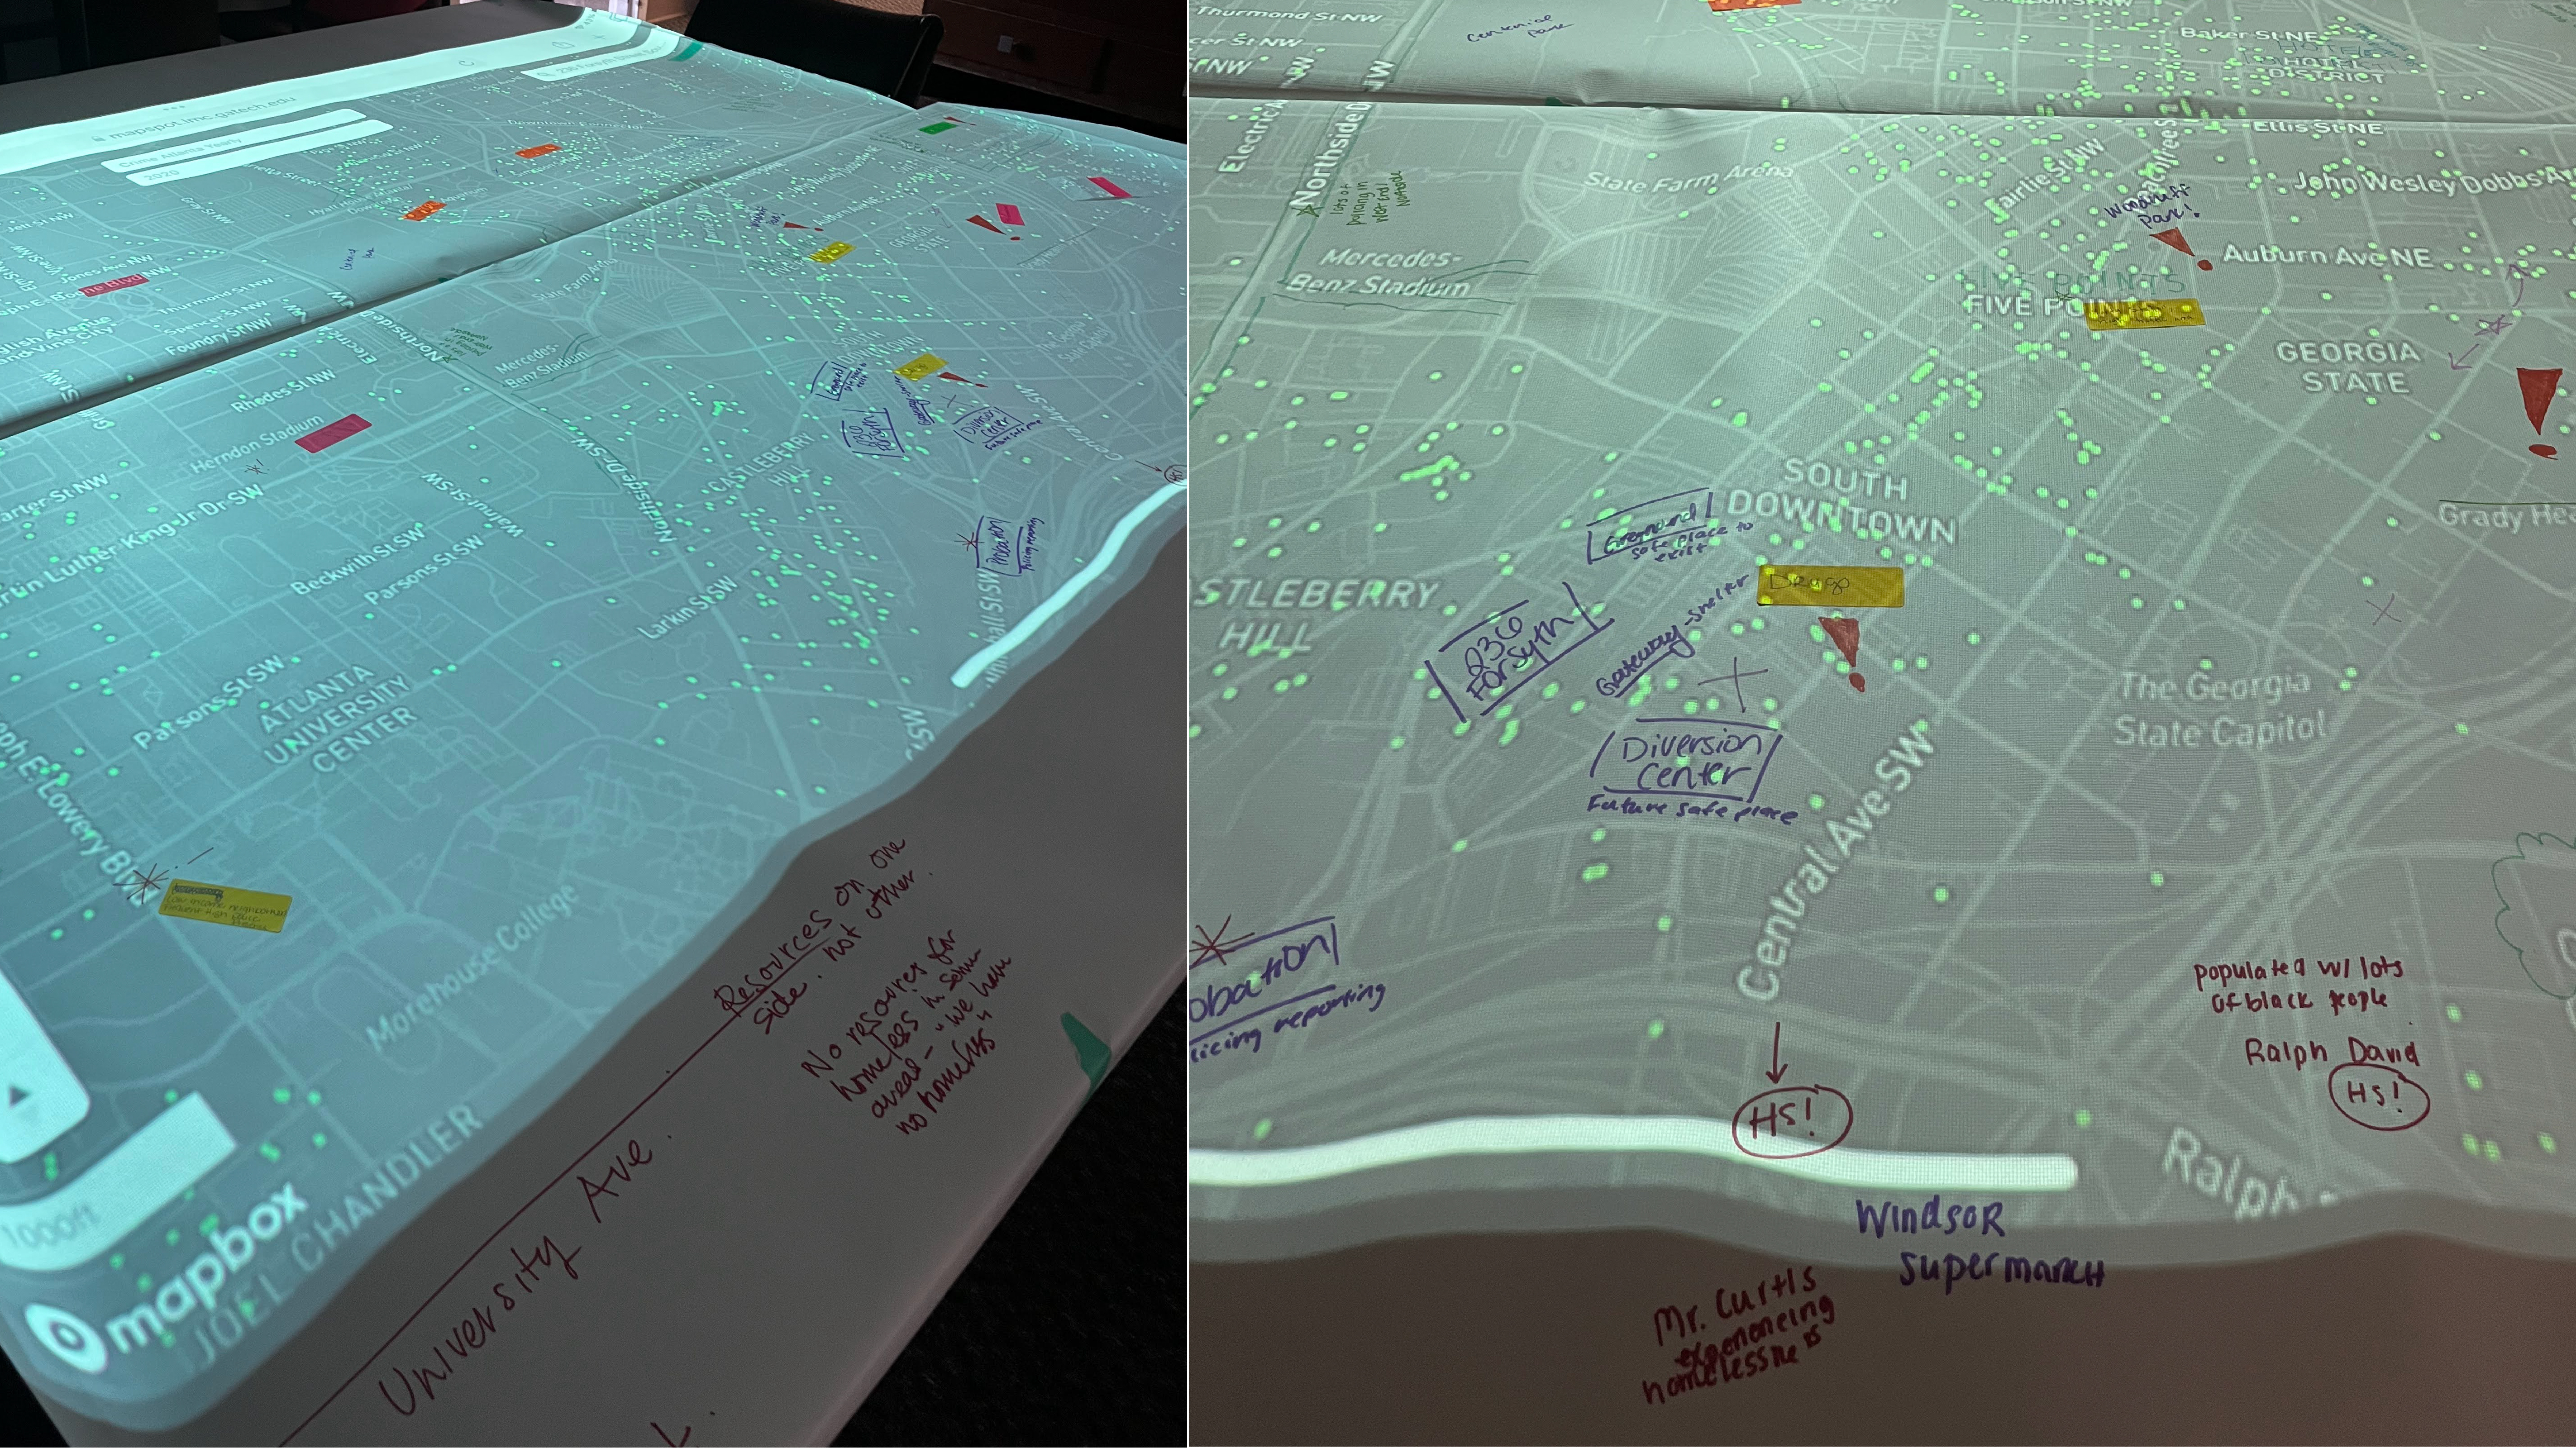
\includegraphics[width=0.99\linewidth]{chapter4_methods/sections/images/Map_closeups.jpg}
         % \caption{John Snow's map that traces the spread of Cholera deaths during London's 1854 Cholera epidemic}
         \label{subfig1}
    \end{subfigure}
% \hfill
    % \begin{subfigure}[b]{0.49\linewidth}
    %      \centering
    %      \includegraphics[width=0.95\linewidth]{images/Snow-cholera-map_resized15.jpg}
    %      % \caption{}
    %      \label{subfig2}
    % \end{subfigure}
% \hfill
% \centering
% \includegraphics[width=0.45\textwidth]{images/REDUCEDD_Snow-cholera-map}
\caption{
    Participatory Maps Close-ups
}
\label{fig:inundation}
\end{figure}
% \end{wrapfigure}
% \ref{fig:choleramap}

W1 invited twelve members of a police reform group that offers supportive services to those experiencing extreme poverty, problematic substance use, or mental health concerns, with the goal of reducing their arrest and incarceration rates. This workshop was conducted in October 2023 in the offices of the partnering organization in Atlanta. Before the workshop, I conducted a 30-minute call with the director of the group to understand their goals, motivations, and expectations of the workshop. 

In their survey, participants reported that they want to learn about the new and advanced methods in policing, what is AI and how AI will be used to promote public safety, how to use these tools responsibly, and how it can help them better serve their communities. A few of them explicitly stated that they had concerns about the use of AI in policing, especially because of the effect of racism on policing, and saw this workshop as a place to discuss those concerns. Participants described themselves as having 'none' to 'very little' knowledge of AI. Two mentioned their use of ChatGPT and another talked about their knowledge of policing technologies like surveillance cameras. 

\subsubsection{Workshop 2: Urban planners} 

\input{chapter4_methods/sections/figures/W2}

W2 invited seven members of a regional civic planning agency in Atlanta.  It supports the leaders of Atlanta in using data-driven methods to plan, invest, and addresses critical issues for the betterment of city's collective future. The workshop took place in the first week of November 2023 in the offices of the organization based in Atlanta. 

Participants were interested in learning about how AI can be used for the betterment of the city and promote equity. They mentioned their roles as urban planners and designers and sought knowledge of civic AI tools to skillfully engage with these tools in their professional work.  Five participants described themselves as being familiar with AI through podcasts, readings, use of ChatGPT, their own work, or the work of those around them. The group seemed excited about the opportunities offered by AI but wanted to learn about how to design, deploy, and use sch tools in an equitable manner.  

\subsubsection{Workshop 3: Open Call} 

\input{chapter4_methods/sections/figures/W3}

Unlike the rest of the workshops, W3 was an open call workshop publicized via a webpage, email, and flyers with neighborhood association leaders, board members, and other neighborhood and civic groups. Folks were encouraged to share and publicize the workshop details to anyone in their network who they deem would be interested. The workshop received seventeen registrations of which seven people participated in the workshop. The workshop was organized on the Georgia Tech campus in mid November. 

This workshop saw a wider range of people. The participants included researchers and practitioners from both academia and civic organizations for neighborhood improvement. One participant worked in violence prevention in Atlanta and another was leading a neighborhood public-private partnership aimed at making spaces better for citizens.  In the survey, some described themselves as ``Pretty familiar with usage" of AI tools and others as ``Not very familiar" with AI. Some had friends who worked in AI and others had used tools with predictive features. Participants were interested in how AI could be used for civic purposes in responsible ways. Two participants were aware of the biases that can creep into AI systems and considered the workshop a space to learn and talk more about it. This workshop was met with a technical error where our short-throw projection on the table stopped working and I, along with my co-moderator, improvised to a wall displayed map. 

\subsubsection{Workshop 4: Community development organization} 

\input{chapter4_methods/sections/figures/W4}

W4 brought in eleven members of an organization that leads, manages, and funds local, community-centered projects across Georgia. This workshop was organized as part of an annual retreat for the organization members where members gathered to discuss strategy for the rest of the year. The organization director met with me before the workshop and considered the workshop timely and useful for members to understand how AI systems may affect the city. Such an understanding, the director hoped, would support their work in civic development for the smart city. The workshop was organized in their offices in early January 2024. 

Most people were participating as the workshop was included as a part of their team retreat. They were interested in incorporating the learnings from the workshop into their work. Participants mentioned different predictive tools they were familiar with. Three participants mentioned variations of ChatGPT, Claude or Bard while some talked about Google maps and Google translate. Overall, the group presented themselves as being familiar with AI through various articles they read, tools they have used, collaborations with AI researchers, or their own work in smart cities. One participant described their interest in learning how to make these tools transparent to the public. Another talked about the privacy and safety of these tools rural communities. 


\subsubsection{Workshop 5: Non-profit of educators} 
\input{chapter4_methods/sections/figures/W5}

W5 invited a group of eight teachers who came together as a non-profit aimed at forming meaningful relationships and collaborations between educators. The non-profit leaders offer experiences to support teachers in their work and, with this workshop, hoped to come together to learn more about AI and its effects on cities. The workshop was organized on the Georgia Tech campus in late January 2024. 

Participants wanted to learn how to responsibly incorporate AI in their teachings, especially with the rise in generative AI and its effect on education. Two teachers taught geography, another taught social science. One participant said they had ``not given AI a great deal of thought", while another participated in a school committee to discuss AI use in high school education. 

 Three of the five workshop partners posted about this work on their social media channels reflecting on their experience and demonstrating the impact the workshop had such as: 

\begin{quote}
    ``As we look to the future of these technologies, we have the potential to enhance community well-being and resource distribution, but only if we fully understand their potential and limitations.'' (W4)
\end{quote}

\begin{quote}
   ``Our engagement [through the workshop] not only broadened our understanding of the power of maps and the ethical implications of AI but also served as a reminder of our role as educators in shaping future perspectives.'' (W5)
\end{quote}



These workshops together inform the rest of the work discussed in this dissertation. I analyse these workshops through two primary methods (1) situational analysis and (2) thematic analysis and memo-ing which I discuss in Chapter 4 and Chapter 5 respectively.
    
\chapter{Situated Explanations and Related Contexts\label{ch4:situated}}

In the last chapter, I discussed how explanation needs are situated in diverse explanation contexts. These explanation needs inquired not just about the predictive tool but also the complex systems that such tools become a part of. As such, this chapter asks: \textit{How can we move towards a better understanding of the expansive and complex socio-technical assemblages underlying AI systems?} 

AI systems emerge out of broad networks of materials, relations, cultures, institutions, and histories that may affect societies in unjust and harmful ways. In this chapter, I argue that local publics can partially explain how algorithms interact with society to affect local contexts. I report on our efforts to engage with these diverse partial explanations through the participatory mapping workshops detailed in \Cref{ch3:methods}. I find that partial explaining can (1) collectively advance our understandings of AI systems as socio-technical assemblages, opening up novel critical questions about these systems, and (2) identify gaps in current algorithmic explanations thereby creating explanation needs that we can attempt to collectively address. I call for the creation of spaces and systems where such engagements of partial explaining and knowing can happen. 

\section{Introduction}
\emph{How can the Explainable AI (XAI) community support public understanding of the spatial workings and effects of civic predictive systems?} 

Civic predictive systems, or systems that affect civic processes, are becoming an inseparable part of the urban smart city.  They inform several fundamental decisions that govern our everyday lives: who gets parole, bail \cite{arnold}, or economic and social aid \cite{noriega2020algorithmic}; who gets hired \cite{raghavan2020mitigating}; how are students assigned to public schools \cite{robertson2021modeling}; how well are teachers performing \cite{teachereval}; which child welfare calls need immediate attention \cite{chouldechova2018case, cheng2021soliciting}; how un-housed people receive housing resources \cite{kuo2023understanding}; who gets a loan application approved \cite{schoeffer2022there}; or which routes we, or our public transports, take in a city \cite{gupta2022rethinking, goodman2019challenge}. They are pervasive. 

The use of predictive systems has been presented as making civic processes more efficient, accurate, and objective. They can effectively and quickly process large amounts of data about a variety of subjects and their environments.  They can identify patterns not previously known while attempting to overcome biases in human-based decision-making \cite{brauneis2018algorithmic}. The hope is that the use of such systems can address the resource constraints within the public sector by off-handing or automating labor, thereby reducing costs and increasing resource allocation capacities \cite{levy2021algorithms}. 

Despite their proposed vision and goals, several civic predictive systems have been shown to cause societal harm and discrimination \cite{eubanks2018automating}. There are countless examples of bias \cite{bartlett2022consumer, dastin2022amazon}, disregard of civil rights and liberties \cite{de2020states, johnson2023face}, or privacy invasions \cite{ice}. The centralized and authoritative nature of algorithms gives them the power to create or reinforce unjust (and often invisible) societal structures and inequalities \cite{d2020data}.  

Geospatial civic algorithms specifically, that make predictions about spaces in the smart city, attempt to fit highly complex cities into neat structures demanded for computation \cite{mattern2020city}. Critical geographers, such as Schwanenand and Kwan, demonstrate how social discrimination and marginalization are inherently entangled with space \cite{kwan2012critical}. The overly simplistic mathematical representation of cities creates the kinds of invisible inequalities and incremental injustices that produce large-scale societal effects, such as gentrification and segregation \cite{loukissas2022wants}. Numerous cases exemplify the inequitable spatial effects on diverse communities:

\leftskip 20pt
\rightskip 0pt plus 1fill
\vspace{8pt}

Planning algorithms such as the Market Value Analysis present governing bodies with a “data-driven objective” means of distributing public resources by classifying and segregating communities through the construction of color-coded boundaries. Such organization of space, as Safransky argues, standardizes unjust classification systems and restructures the public sphere in ways that favor some neighborhoods over others. These civic algorithms are opaque, inaccessible, and are rarely if ever, developed through a public and participatory process \cite{safransky2020geographies}.

Sociologists such as Zukin et al. have demonstrated how geographically coded Yelp reviews reinforce prejudice against neighborhoods with people of color thereby influencing civic investments and contributing to processes of urban change such as gentrification. The algorithmic moderation of reviews is not public, and users are unaware of their role in affecting capital flows \cite{zukin2017omnivore}.

Loukissas argues that filter bubbles created by Zillow reinforce existing spatial power structures along the axes of race and class. Even as the goal of the site is to give users more control over their home-buying experience, it leaves users unaware of the implications of their own filtering decisions \cite{loukissas2022wants}.

In my past work, I illustrate how safe walking apps, such as Safetipin, risk segregating neighborhoods by attempting to advance the safety of one social group while marginalizing another. Once again, knowledge about the failings of social structures and policy normalized by the app is inaccessible to citizens, as well as the app creators \cite{gupta2022rethinking}.

\leftskip 0pt
\rightskip 0pt 
\vspace{8pt}

Without careful consideration of the spatial workings and effects of predictive systems, they risk reproducing or even amplifying historical systems of discrimination. Currently, civic algorithms are deployed in ways that prevent citizens from getting access to them or learning about their existence and effects. This limits the citizens' ability  to contest, oversee, assess, or protest automated decisions that affect their lives in fundamental ways. To address concerns of algorithmic opaqueness and lack of understanding, activists \cite{stop_lapd}, civic organizations \cite{lee2023making,post}, as well as several governmental agencies \cite{white2022blueprint} are calling for advancements in algorithmic transparency, explainability, and impact assessment.  Their goal is to drive visibility into the design of algorithms, opening them up for critique and evaluation by both experts and everyday users.  

\section{Existing XAI and AI Transparency Approaches}

Early research on Explainable AI focused majorly on technical explainablity and transparency. For black-boxed algorithms, post-hoc explanations where another human-interpretable model imitates the practices of a complex model are being designed to understand how an algorithm makes its predictions. Guidotti et al. \cite{guidotti2018survey} categorize post-hoc explanations into these categories: (1) Global Model Explanations where a simpler interpretable model is trained on the same data to approximate the working of the primary more complex model, (2) Outcome Explanations where the focus is on explaining one outcome or instance of prediction by providing the weight of features that contributed to it \cite{schuff2022human} or examples of inputs that would lead to a similar prediction, and (3) Counterfactual Explanations where the goal is to identify what should be changed in the inputs to get a different prediction \cite{shang2022not}. Beyond making models interpretable, XAI efforts attempt to make known other aspects of the machine learning model such as datasets, training algorithms, source code, and performance metrics \cite{vaughan2020human}. Several model \cite{mitchell2019model} and data documentation \cite{anik2021data, bender2018data, gebru2021datasheets, holland2020dataset} frameworks, have been designed to explain AI to experts \cite{dhanorkar2021needs}. Frameworks such as `CrowdWorkSheets' support standardized documentation of decisions when annotating datasets in a crowdsourced manner \cite{diaz2022crowdworksheets}. `Data Cards' provide summaries of datasets for various stakeholders \cite{pushkarna2022data}. To promote transparency of models, existing work proposes tools such as `Model Cards' that aim to provide details about a model related to its working, use cases, and evaluation \cite{mitchell2019model} and `Factsheets' that provide an overview of facts about specific models across the AI lifecycle \cite{richards2021human}. There is also growing work in designing open-source toolkits to identify and assess algorithmic harms and biases \cite{bellamy2018ai, wexler2019if, bird2020fairlearn}. AI Fairness 360 (AIF360) \cite{bellamy2018ai} and Fairlearn \cite{bird2020fairlearn} are tools that aim to help practitioners understand `bias' metrics and allow them to detect algorithmic biases. These tools also help mitigate said biases by providing a variety of mitigation algorithms. Another tool called ``What-If'' uses visualizations to help users and practitioners investigate how a model will perform in hypothetical scenarios created by changes in data points \cite{wexler2019if}.

More recently, the XAI community has presented the need to make AI processes visible to the general public in order to build trust in the artificially intelligent systems that guide their lives \cite{knowles2021sanction}. There has been a growth in work that focuses on developing methods and frameworks for user-centered algorithmic explanations \cite{miller2019explanation, shneiderman2020human, vaughan2020human}. Human cognitive abilities \cite{wang2019designing}, users' explanatory needs \cite{liao2020questioning, springer2020progressive}, users' situated real-world experiences \cite{devos2022toward}, users' ability to collaborate and form counter publics \cite{shen2021everyday} have been some of the guiding factors in advancing user-centered XAI research.    

Such efforts have built on diverse theories and methods: interactive explainability methods \cite{cheng2019explaining}, such as Interactive Model Cards \cite{crisan2022interactive}, have been proposed, theories describing human cognition patterns have been employed \cite{wang2019designing}, and example-based methods where data samples that informed a prediction are shown to users have been presented as helpful \cite{cai2019effects}. Additionally, several toolkits have been designed to promote user understanding of AI systems such as: TILT (transparency information language and toolkit) that organizes the information that transparency policies demand in structured ways for machines to read and users to consume \cite{grunewald2021tilt}, or AIX360 toolkit \cite{arya2019one} that present visualizations and explanation algorithms respectively to help users understand how predictive systems work. Investigations into how XAI can support user assessment \cite{robertson2022understanding} and decision-making capabilities \cite{kulesza2013too} are also being conducted.

These efforts have made monumental progress in the field of Explainable AI. Yet, there remain limits. First, they are not pluralistic in nature \cite{hancox2021epistemic, ehsan2022social} and do not consider the values, surrounding social systems, existing knowledges, and beliefs \cite{kaur2022sensible} of users in the design of explanations. Second, they may focus merely on technical transparency, disregarding the systemic factors surrounding any algorithmic decision \cite{ehsan2021expanding}. Third, they tend to be one-time explanations that portray users as passive individual consumers \cite{corbett2023interrogating}. And lastly, the goal of most explanations is to increase user trust rather than to promote critical thinking or action \cite{danry2023don}.  This leaves little room for democratically evaluating how the complex world we live in is simplified to be represented in the design of algorithms— who is included, who is excluded, and how cities are quantified and aggregated for computation. I discuss these limits in more detail in \ref{ch2:gee}. 

This dissertation aims to address these limits and theorize the design of effective public explanations of civic AI tools. I want to note that in using the term `explanations', I am not referring to the technical explanations provided through the use of algorithmic interpretability methods. Rather, I am attempting to expand our community’s understanding of `explanations' such that it is not limited to the technical understanding of the systems but is explaining the social, political, and economic development, use, and effects of civic predictive systems. 

I ground my work in public safety AI systems. Specifically, I employ place-based predictive policing as a case study for this research.


\section{Public Safety Algorithms and Harms }  

My research for this dissertation started with a critical analysis of a renowned safe walking app, primarily deployed in India, called `Safetipin' \cite{safetipin}. Safetipin recommends `safe' paths to users from an origin to a destination by calculating `safety scores' for various paths. These safety scores are calculated by aggregating crowdsourced `safety data' such as the amount of lighting, or presence of security officers, in various locations in a city. To study this tool, (1) I draw on feminist criticisms of safety technologies, defined broadly, to identify the main issues in their framing and efficacy, and (2) I build upon initial interviews with users and makers of Safetipin to examine how the app addresses, or fails to address, the criticisms received by other safety technologies.

This critical analysis demonstrates Safetipin’s capacity to (1) restrict women’s movement to computationally calculated `safe' neighborhoods and (2) reinforce caste and religion-based segregation in India \cite{gupta2022rethinking}. By disregarding the prejudice about vulnerable neighborhoods that governs the `feeling of safety' of its users who contribute to the crowdsourced data, Safetipin fails to situate itself in the broader historical politics of safety in the city \cite{kern2021feminist} that continue to marginalize people of lower socioeconomic status and minority religions. Nonetheless, the app and its underlying information infrastructures that promote segregation, have been enthusiastically accepted and celebrated \cite{safetipin_award1, safetipin_award2}. This work presents a dire need to identify and understand the impact of spatially distributed data inputs and aggregations on the city and its people. Ultimately, it motivates the need to explain how emerging civic geospatial technologies, especially in the realm of public safety, organize cities and their impact on spatial segregation and discrimination. 

Amongst other tools for public safety exist a variety of ML algorithms that have been developed with the hope to mitigate crime and advance citizen safety in smart cities. Popular examples include— COMPAS \cite{compas}, which predicts recidivism risk for an individual; Predpol (now Geolitica) \cite{predpolbad}, which predicts geographic areas where crime is most likely to happen; Arnold Public Safety Assessment \cite{demichele2020public}, which provides judges with sentencing recommendations. These algorithms, even as they aim to promote public safety in cities, tend to reinforce discrimination along the axes of race and class. Jefferson demonstrates how Predpol legitimizes the bias embedded in official crime datasets and has resulted in the over-policing of already heavily surveilled neighborhoods \cite{jefferson2018predictable}. Risk assessment tools build upon and reinforce the racist policies and infrastructures underlying carceral systems in the US. Additionally, they define `risk' at the level of an individual, disregarding how `risk' is a reflection of societal prejudice against various social groups \cite{green2020false}. In India, centralized systems and norms along with the subjectivities of individual police officers lead to historical, representational, and measurement bias in recorded crime data for the Crime Mapping Analytics and Predictive System (CMAPS) predictive policing tool. Further, the opaque design of CMAPS allows for discrimination against immigrant colonies and minority settlements by promoting the belief that crime rises in specific neighborhoods by virtue of the above-mentioned communities living there  \cite{marda2020data}. Transparency is a much-needed feature for the effective assessment and development of public safety algorithms \cite{rudin2020age}. Given the limited potential of techniques designed to “de-bias” public safety algorithms, there is an urgent need to make the data assemblages \cite{kitchin2014towards} surrounding public safety algorithms transparent and accessible to city residents and governmental bodies \cite{marda2020data}.   

This dissertation aims to study the concept of effective public explanations,  by specifically focusing on place-based predictive policing as a case study. Place-based predictive policing is a method that aims to support the efficient distribution of police resources in a city. Typically, the method utilizes historic crime data such as arrest reports or calls for service requests integrated with other social and environmental data to predict the location and time of future crimes. A popular example of such a system is called Geolitica (previously Prepdol) \cite{predpolbuy}. In the past decade, academics and activists have heavily scrutinized the use of predictive policing \cite{o2017weapons}. The tool has been shown to reproduce existing geographic and social biases embedded in historically discriminatory crime data \cite{jefferson2018predictable,akpinar2021effect}. A recent study conducted by the Markup has found the accuracy of this tool to be less than half a percent \cite{predpolbad}. Many others have discussed the incompleteness of data \cite{kirkpatrick2017s}, the inability to validate results \cite{demortain2017evaluating}, and the proliferation of positive feedback loops \cite{o2017weapons}. Such thorough investigation of this predictive tool makes it an ideal case to ground our discussions of effective public explanations. 



\section{Research Questions and Chapter Outline}

In this dissertation, I ask: \emph{How can the XAI community support public understanding of the spatial workings and effects of civic predictive systems (RQ)?} To investigate this question, I primarily employ community-centered qualitative and participatory methods. Additionally, I build on and am in conversation with scholarship from fields such as human-computer interaction (HCI) that investigates how users perceive, relate to, and interact with AI systems to seek AI explanations; science and technology studies (STS) that shines light on the socio-technical environments surrounding AI, publics affected by AI, as well as the processes of explaining and knowing; and AI Transparency and Explainability (XAI) that has designed numerous methods, frameworks, and tools to explain AI systems to a variety of audiences. 

\Cref{ch2:gee} begins my investigation of the primary research question guiding this dissertation (RQ) by asking: \emph{ What qualities underlie effective public explanations of civic predictive systems (RQ1)?} My inquiry is driven by a semi-structured interview study along with an extensive review of existing scholarship on public explanations for civic predictive systems. I interview 23 participants including academics, AI activists, journalists, community and neighborhood leaders, and civic society organizations who think, write, or act on issues of social justice and AI safety, to identify the qualities and characteristics underlying meaningful public explanations of civic predictive systems. Drawing on my findings, I introduce the concept of \emph{ ‘good enough explanations’}. ‘Good enough explanations’ as understood by our participants, (1) are \textit{situated} in the lives of diverse publics, (2) explain the complex and entangled socio-technical \textit{systems} that predictive tools interact with, (3) involve \textit{continuous and partial} processes, and lastly (4) empower publics to \textit{act} in ways that promote democratic deployment and regulation of predictive tools. Such explanations, I argue, may not be complete or objective but are good enough to support publics in critically engaging with the workings and effects of civic predictive systems in service of their goals. The rest of the dissertation attempts to understand and explore these qualities.  

\Cref{ch3:methods} documents my approach to study, as well as create, good enough explanations. \textit{Form} has been considered an essential dimension of AI Explanations \cite{van2021effect}. As such, I take inspiration from the visual history of city representation to demonstrate how \textit{mapping} may allow us to explain geo-spatial AI systems in ways that are accessible, culturally reflexive, situated, and provide visibility into how algorithms represent cities. I employ a `research through design' methodology and conduct participatory mapping workshops with diverse publics such as— police reform groups, city planners, neighborhood and community leaders, civic development agency, and educators— to investigate how can we, as XAI researchers, design good enough explanations. The workshops encouraged participants to question, understand, and explain place-based predictive policing on their own terms by using maps to ground discussions in the spaces they live and work in. The explanation contexts that emerged were analyzed using inductive coding, situational analysis, memo-ing, and thematic analysis. These workshops support the findings and arguments developed in chapters 4, 5, and 6.

\Cref{ch4:situated} studies the `situated' nature of public explanations and asks: \emph{How are explanations situated in the lives of diverse publics and what does that mean for the design of public explanations (RQ2)?} Drawing on five participatory mapping workshops with diverse publics, this chapter reflects on the explanation contexts that emerge when publics question or understand AI systems. I find that when attempting to understand AI systems, publics draw on their relation with not just the predictive technology, but also the prediction domain, prediction subject, and prediction backdrops. Situated explanation needs of publics emerge out of these entangled relations. I argue that these broader relations play a significant role in supporting public understanding of civic AI systems and urge XAI researchers to consider these relations as they attempt to design systems for public understanding of AI. 

Chapter 5 studies the `systemic' nature of public explanations and asks: \emph{How can the XAI community help explain the complex socio-technical systems that civic AI tools engage with?} Underlying AI systems are socio-technical assemblages of materials, relations, cultures, institutions, and histories. In this chapter, I analyse the participatory mapping workshops using situational analysis to demonstrate the ability of local publics to partially explain the environments AI tools are deployed in, the cultures and norms they invade, and the lived experiences of the problems they attempt to address. Drawing on these findings, I argue that good enough explanations need not be designed in isolation \emph{for} publics \emph{by} XAI researchers. Instead, XAI researchers would benefit from co-creating systemic explanations \emph{with} diverse local publics through slow and long-lasting engagements.  

Chapter 6 reflects on the methods I use to develop good enough explanations to reconceptualize explanations as explain\emph{ing}— a continuous and partial process that supports the development of \emph{situated} understandings of AI \emph{systems}. I provide a detailed account of three design dimensions I believe should be considered as XAI researchers design spaces and systems that mediate processes of explaining: (1) designing explaining sites (2) designing explaining media, and (3) designing explaining interactions. I briefly discuss how explain\textit{ing} may influence public `action'. I end by providing a list of questions that XAI researchers can consider as they attempt to create good enough explanations for civic predictive systems.  

Lastly, I conclude by providing a summary of the research conducted in this dissertation, highlighting limits of this work, proposing relevant future work, and positioning the work in relation to my background and motivations. 

Together, these chapters attempt to make three primary contributions to the field of XAI: (1) theoretical contribution by conceptualizing what \emph{good enough explanations} mean for public understanding of civic predictive systems, (2) empirical contribution by reporting how diverse publics may understand, question, and explain civic predictive systems, and (3) methodological contribution by demonstrating and recommending strategies for co-creating a good enough understanding of civic predictive systems.  

My hope is that this work will support XAI researchers, policymakers, and community leaders in designing systems and spaces for public engagement with civic predictive systems. Such engagements, as stated in \Cref{ch2:gee}, should work to promote democratic public action toward contesting, redesigning, regulating, or discontinuing predictive systems that may cause societal harm in fundamental yet currently invisible ways.  

 
% text of this chapter goes here

\section{Background}
\subsection{Exiting methods to explain AI systems as socio-technical assemblages}

Majority of existing efforts to explain AI focus on technical components such as algorithmic features and their weights, training datasets, source code, and performance metrics \cite{vaughan2021human}. Recently, the XAI community has called for moving beyond technical transparency and considering other socio-technical elements impacting AI decision-making. Few but growing frameworks and concepts are being proposed. Ehsan et al. introduce social transparency, which includes making transparent the technological context, decision-making context, and organizational context surrounding algorithms \cite{ehsan2021expanding}. Similarly, Kroeger et al. account for user literacy and propose ‘social explainability’ as a concept that explains not just the AI system but the AI ecosystem \cite{kroeger2022social}. They argue that insight into the institutional systems that AI becomes a part of can help users trust the institutions deploying AI even if they do not understand how an AI tool works \cite{kroeger2022social}. Cobbe et al. argue that current XAI methods provide insufficient information to regulate AI systems and propose ‘reviewability’ as a framework for more meaningful transparency across the entire AI lifecycle \cite{cobbe2021reviewable}. Geiger et al. use a “sociotechnical systems approach” and propose reimagining ‘audits’ as tools that don’t settle ‘matters of fact’ but instead that open up investigation into ‘matters of concern’ \cite{geiger2024making}. Such a change in perspective, they urge, will prompt us to ask questions about algorithmic systems in relation to the organizations that deploy them. Yu-Shan Tseng specifically focuses on Urban AI and proposes ‘assemblage thinking’ as a methodology to study the relations between algorithms and the cities they are situated in \cite{tseng2023assemblage}. They present a case study of vTaiwan, an open-source algorithmic platform, as situated in complex urban assemblages. They describe in detail its political and collaborative origins and how it creates communities for democratic engagement. 

Community-centered methods have also been proposed or employed to study AI systems as socio-technical assemblages. Rob Kitchen echoes the need to study algorithms as situated in broader socio-technical assemblages. He recommends conducting interviews and ethnographies of particular AI systems to shed light on the principles they adhere to \cite{kitchin2019thinking}. Seaver proposes using ethnographic methods, living with-in algorithmic systems, to know not just how algorithms work, but how they come to be \cite{seaver2019knowing}. Stop LAPD Spying Coalition worked with an activist organization called the Free Radicals and investigated the use of Predpol in Skid Row, a community in downtown Los Angeles. They proposed a framework called the ‘Algorithmic Ecology’ that maps, visualizes, and communicates the relationships of power that surround any algorithmic technology \cite{stoplapd}. 

Researchers and artists have attempted to visualize the socio-technical nature of AI systems for better user understanding. Kate Crawford and Vladan Joler designed a visualization titled ‘Anatomy of AI’ that traces AI throughout its lifecycle and makes transparent the resources that help develop an AI system \cite{crawford2018anatomy}.  

These works motivate the need to understand AI systems as complex and entangled networks of social, historical, cultural, and technical components. I add to this rich foundation of methods to explain AI as socio-technical assemblages.  


\subsection{Explaining AI systems by local publics }

Another shift in XAI efforts has been guided by the desire to move beyond merely ‘experts’ providing explanations to ‘non-experts’. Experts, from their own standpoints, are positioned well to explain specific parts of AI systems. However, scholars are increasingly recognizing the need to engage with the public to understand the effects of algorithms. Eyert and Lopez’s ‘transparency as a communicative constellation’ calls for multi-directional transparency where tech experts don’t just teach, but listen and learn from publics \cite{eyert2023rethinking}. In a similar vein, Nicenboim et al. call for co-creating an understanding of AI systems with both users and artificial agents \cite{nicenboim2022explanations}. They argue that explanations and methods of understanding offered by citizens are no less legitimate than the explanations offered by experts. Engaging with external actors and diverse publics can help identify relevant algorithmic concerns and needs \cite{nicenboim2022explanations}. Sloane echoes these values and presents participation by a more diverse set of actors, especially in ways that are “unscripted, unpredictable, and are beyond the grasps of bureaucratic control”, as a technique to ‘unblackbox’ AI systems \cite{sloane2024controversies}. Corbett and Denton join fellow researchers and respond to the technocentric turn that the XAI communities have taken, by making calls for ‘bringing people to transparency’ \cite{corbett2023interrogating}. ‘Participatory AI’, as defined broadly, provides various degrees of power \cite{corbett2023power} to the public to inform the design, use, assessment \cite{blair2019exploring}, advocacy \cite{krafft2021action}, and governance \cite{seger2023democratising} of AI systems. 

Growing, but still nascent work, has involved users as experts who can explain AI systems. Barnett and Diakopoulos propose crowdsourcing as an effective method to anticipate societal algorithmic harms \cite{barnett2022crowdsourcing}. They utilize the diversity of Amazon Mechanical Turk workers to describe the impact domains of algorithms used by the U.S. government. Marian presents a brilliant case study where parent groups and researchers come together to understand the (New York City) NYC School Matching Algorithm \cite{marian2023algorithmic}. The authors crowdsourced information about the lottery numbers that students received and the schools they were matched to understand the role lottery numbers play in the matching algorithm and identify cut-offs for various schools. Their results were made available publicly to help keep student applicants in the following academic years informed about how the system works. Other `citizen-science' projects have attempted to gather distributed information about technological systems. The `ban the scan' project by Amnesty International mobilized volunteers to share information about the presence of surveillance cameras on the streets of NYC and Hyderabad \cite{banthescan}. By doing so, they were able to explain the omnipresence of discriminatory facial recognition systems and call for a policies that ban these tools. These examples of crowd sourcing are inspiring starting points. However, they are still driven by researchers and not publics. This does not allow publics to draw on their multi-faceted expertise. Rather they provide information as requested by the researchers. They involve publics only to the extent that they can provide experiential data points without considering them experts of their own elements in the broader AI system. 

I build on these works described above in three ways: (1) I provide publics with an open platform to explain distributed parts of an AI systems based on their expertise, (2) I bring the expertise of diverse publics together instead of focusing on one aspect explained by one stakeholder type and , (3) I focus on nuanced grounded explanations instead of factual data points.   


\section{Data Analysis}
This chapter aims to investigate if and how local publics can partially explain elements of AI systems in the capacities in which they interact with these systems. To do so, I start with identifying and pulling out instances of partial explaining and questioning from the workshops to form a repository. Next, I write memos \cite{bernard2017research} reflecting on if and how this explanation can help us better understand AI systems as socio-technical assemblages alongside novel questions that it opens up. 

This was followed by a reflexive thematic analysis \cite{braun2019reflecting} where I categorized partial explanations offered by publics into elements of AI systems that they explained such as—spatial, social, relational, historical, policy, lived, etc. Through further refinement of these themes I identified the categories of explanations that organize the findings section below. These categories are not exhaustive or mutually exclusive but serve as an example of the variety of partial explanations users can provide about socio-technical AI systems. 




\section{Findings}
In this section, I report on the explanation contexts that emerged as I mediated processes of knowing and explaining predictive systems. Out of the five workshops I conducted, I briefly describe partial contexts of Workshop, 1, 4, and 5. These workshops serve as good exemplary cases for this work. 

\subsection{Workshop with police reform group (W1)}

W1 invited twelve members of a police reform group that offers supportive services to those experiencing extreme poverty, problematic substance use, or mental health concerns, with the goal of reducing their arrest and incarceration rates. At the beginning of the workshop, participants expressed their feelings toward predictive policing tools calling them \emph{“really terrifying”} and \emph{“scary”}. Their fear was driven by \emph{“rights issues”, “reading of cases of people being exonerated from convictions with AI-based evidence”, AI being “rolled out so fast”, “need for compassion in policing that AI lacks”, ability of AI to “decide the outcome of someone’s life and future”}. These feelings of concern motivated their presence and desire to know more about the workings and effects of predictive policing tools. Their collective skepticism towards predictive tools including \emph{“facial recognition"}  or  \emph{“ads”} drove their fear of place-based predictive policing. 

Owing to their position in and relationship with the institution of policing, they were highly skeptical of technology usage in policing. They firmly believed that ‘crime’, as defined by the law and police departments is unjust. As such, they inferred what crime would mean for predictive systems. They said:
\begin{quote}
    “[Our] definition of crime is very different than what AI systems refer to as crime. So, like drugs are not crime to us. So, this [predictive system] is a lot about like tracking drugs. But we think drugs are a public health issue and not a safety issue.” 
\end{quote}
Concerned that police may categorize public health issues as crime, they asked what definition of crime is the predictive tool using. They questioned the motives of predictive systems: \emph{“If you are going to criminalize these public health issues then it may be more beneficial to predict where there will be these public health issues”}. The intentions of the tool— to arrest people or help them— dictate the predictions a tool makes and the policing actions that follow the predictions. 

Drawing on their experiences working with and living in diverse communities, they discuss the disparity in neighborhoods. The relationship of the neighborhood residents with each other and their collective relationship with the police would directly affect the workings of predictive tools. They explain: 
\begin{quote}
    “What we see on a daily basis, areas like Buckhead, they give us the most referrals for criminal trespassing, and it could just be an unhoused person sitting in the park in the middle of the day. They just don't wanna see them. But on the south side, the more impoverished communities, we don't get calls like that for unhoused people because they are friends and family, they don't look at them like criminals and they support them.  My mom calls the person on 11 and 23 on Cambleton road, she calls him uncle. I know his face and can point him out. If you are familiar with them, you wanna see them living. You just want them to get help.” 
\end{quote}
Neighborhoods that consider outsiders to be 'threats' are more likely to report them to the police. Another participant builds on this and suggests: \emph{“If you go off of 911 calls you have to see who calls 911. Because not everyone does. So the data is already going to be skewed.”} They present a need to inquire how the data that is fed into predictive tools is collected and whose perspectives does it capture. They fear that disparate reporting patterns, if not acknowledged and addressed, can reinforce harmful policing practices. 

The group emphasizes that it is essential to consider not just the data being put in and the prediction that is the output, but what we do with the predictions: \emph{ “Are they gonna start going out and arresting people or are they gonna use the fourth amendment and protect our rights once that data is gathered. I think it is about controlling the police in a way that protects our rights.”} This opens another explanation need for learning about how police and other stakeholders act on the tool's  prediction. They also discuss what this action means for community trust in police and holding police accountable. A \emph{“disconnect between real events and AI predicting events will add to the distrust in a world where there is already a lot of distrust... how do we prevent them from terrorizing certain areas and hold them accountable for where they decide to go?” } Their worries and questions are grounded in the current state of the institution of policing. They say: \emph{“For predictive policing to have any effect of public safety, policing itself would have to have an effect on public safety...  ” } They ultimately ask about how this specific tool betters or worsens the current state of the institution of policing. 

\subsection{Workshop with civic funding agency (W4)}

W4 brought in 11 members of an organization that leads, manages, and funds local, community-centered projects across Georgia. They considered the workshop \emph{‘timely’}. Unlike Workshop 1 described above, most of the people in this group were \emph{‘cautiously optimistic’} and wanted to understand how they could make the most of predictive technologies while managing their harms. They hoped to deploy technologies to reduce crime and increase economic opportunities in the American South.  

When discussing predictive policing, participants speculated that the tool may drive police officers to areas with petty crime to increase their arrest count. An increase in arrest count may help demonstrate the effectiveness of the tool for wider adoption in the country. Given their understanding of the economic growth needed to fund projects, they expected a report of higher crime and arrest rates to be a financial motivator. However, they questioned whether an increase in arrests would truly promote public safety. This led to them asking:
\begin{quote}
    “I have a question about.. is that [arrest count] the metric police are using to say that they are efficient? I know historically they have used such a metric but recently there have been studies on how that is not the right metric and how arresting people for petty crimes is not the right metric. So, I wonder if police departments have started to shift their metrics that show they are efficient. If they have changed, then this tool may be able to help.” 
\end{quote}

As such, they inquired about the methods used to assess the effectiveness of predictive practices across police departments. They hoped that a more holistic method than 'increase in arrest count', could help prove useful to measure the impact of the tool. However, they stated \emph{“How can you know, all these police departments are autonomous in their own ways so who knows what their objectives are?” } They discuss the challenges of opaque and decentralized police departments that may measure and report their arrest counts or safety impacts differently. 

They draw parallels between crime data or 911 data with 311 data about non-emergent civic issues, such as infrastructure repair. From their work, they are aware that over-reporting of 311-related issues in certain areas draws economic investment there over other places. They ask how disparate reporting patterns may affect crime predictions.

During the workshop, participants marked high crime spots on the map based on their own perceptions of space. They revisit those markings and say \emph{ " we have so many circles here, we have little five points and waterbouys down here ".} They call the marked crimes in those areas \emph{“very minor and visible”} such as \emph{“drug use, which is not a crime that is actively hurting anyone”}. They were trying to make a point about how a quantitative measure of more may not always mean decreased safety for the public. They inquired about how the predictive tool measures the seriousness of crimes. 

The conversation about drug use and crime led a participant to ask \emph{“We have talked about public safety a lot. Have you looked at cities that have started to decriminalize certain things? Some of it is policy right? Historically some crimes should not be classified as crimes and should not be fed into the systems. How do these systems change with ordinances and laws? Like Houston, they decriminalized marijuana and one of their elected officials ran on the fact that arrests went down.” } They asked if such policy changes resulted in data cleaning or not.

In initial introductions before the start of the workshop, the director of the group said that according to her, poverty is the main cause of crime. This was reinforced multiple times in the workshops and led to participants asking \emph{“Are there efforts to predict why people commit crime instead of where? Because then maybe people need food in a certain neighborhood.” “Are we getting people the right services and what do those services look like?” } They asked about how predictive tools could be used to provide care services to those in need instead of arresting them using the force of police. They speculated possible responses together: 
\begin{quote}
    “Crime is too big of a genre .. to think about how we can do this.. There are different types of crimes that may need different responses, maybe we can see the different types of crimes that are happening and if there are pockets of different crimes in different places and deploy different kinds of resources...[another person continues] doesn't that call for partnerships, that's when the community improvement district steps up to work with the department of public safety, that works with the civic non-profit organization, etc coming together, to address a place-based problem that is globalized to a condition.” 
\end{quote}
Through these partnerships between different civic entities, we can begin to address place-based public safety concerns. They wondered how the predictive tool affects such partnerships currently as well as the potential it has in doing so in the future. 

\subsection{Workshop with educators (W5)}

W5 invited a group of 8 teachers who came together as a non-profit aimed at forming meaningful relationships and collaborations between educators. Participants taught subjects such as the theory of knowledge, geography, and high school science in different schools spread out in the city of Atlanta. Many of them were participating to better equip themselves with information on civic AI systems in a world where they are suddenly being \emph{“bombarded by AI”}. Additionally, they sought skills that would allow them to train young minds to be more critical as they grow up in the world of predictive systems.  

The workshop started with a discussion about the goals of place-based predictive policing, i.e. efficient deployment of police forces. Participants talked about their desire for a \emph{“layered response”}. They compared policing practices in the United States with other countries and explained \emph{“here we only have one type of cop with a gun—they are reactive, in other countries, there are cops walking around whose response is not gun”}. They also compared current policing mechanisms with historical accounts: \emph{“I remember when we used to have sub stations... It would be nice to have police on foot who are walking around and getting to know people. Like the oldies. There are programs where police are able to get affordable housing in neighborhoods that have more crime. They used to have it where they built Olympic housing.”} However, a participant explained that the response and its nature would depend on the urgency and the severity of the crime being conducted. This discussion ended with a question about the type of crimes that predictive systems currently focus on or should focus on. Participants ask: \emph{“Are we thinking only of crime that can impact ...when we are thinking of crime, what is the definition of crime?” } As stated above, this question has repeatedly been asked in previous workshops. Deployment of police force was considered appropriate only for severe or violent crimes and therefore, participants wondered, what crimes were being predicted by the tool. 

Continuing the discussion on the type of crime the predictive systems focus on predicting, they recounted recent political crimes, that may be unusual, but very impactful. They asked: \emph{“Are they using it [predictive system] to figure out if next election we will have another charging of the capital? Where are the white supremacists? Are we looking for this?” } They considered how a predictive tool could have been useful in preventing historical crimes of a specific nature and asked if and how was this a possibility for preventing future crimes.

At numerous points during the workshop, participants drew on their own experience of space asking questions about specific neighborhoods. They wanted to know about seemingly wealthy neighborhoods that experience high crime rates. They asked \emph{“What happens in a neighborhood like Buckhead where the income level is quite high but there seem to a lot of crimes like gun shots.. You always hear about the Publix etc. How does that intersectionality work where there is high income but lots of crime?”} With this question, they wanted to know how the socio-political characteristics of a neighborhood may influence crime predictions and that means for the workings of the predictive tool. 

They also asked questions about the effect of changes in neighborhoods, such as social or infrastructural growth or decline, on crime predictions. Early on in the workshop, the group discussed the relation of food deserts, lack of economic opportunities and social resources, and access to healthcare and education, with crime. They observed how different areas in Atlanta are transforming and asked: \emph{ “I would be interested in how neighborhoods have changed over the years and how has that changed the data analytics... I wanna see how adding more grocery stores change an area.. it would be interesting to see what is the impact around Old Fourth Ward since they closed the hospital..” }. By tracking the changes in neighborhoods and their affect on crime, they hoped to identify methods to disincentivize crime by meeting basic human needs.  

Participants asked questions about what safety means for people in diverse neighborhoods. A participant laid out a detailed account where he compared two MARTA stations (MARTA is the public transit train system in Atlanta), East Point MARTA Station and College Park MARTA Station. He described how the College Park MARTA station has several private schools and has a large police force protecting students as they leave school. In contrast, East Point Marta Station, which is within 2 miles of College Park, has seen 2 murders in the last 4 months. Would this, they ask  \emph{“be an argument FOR predictive policing?” }Another participant adds nuance to this \emph{“With the tri-city moms there is a double-edged sword—I want to protect my kids but who am I protecting them from? Themselves or the police?” } They questioned how the presence of police may affect the feeling of safety in diverse neighborhoods. 

Above, I provide a report of the explanations contexts that emerged from meaningful questioning of AI systems.  I demonstrate how publics asked questions in large part due to their feelings about, knowledges of, or experiences with predictive domains (policing), predictive subjects (spaces), predictive backdrop (current events), and predictive tool (place-based predictive policing).  I discuss these relations in more detail in the following section. 



\section{Discussion}
AI systems exist as socio-technical assemblages of histories, cultures, institutions, and practices. AI tools affect and are affected by interactions with these broader networks. How then can we understand these networks and their underlying mechanisms to identify, assess, and regulate AI related social harms? This chapter contributes to existing literature on studying AI systems as socio-technical assemblages by empirically investigating the role that actors inhabiting parts of an AI system can play in partially explaining them. I find that partial explaining by diverse publics can collectively advance our understandings of AI as socio-technical assemblages opening up novel critical questions about them, and identify gaps in current explanations thereby creating explanation needs that we can attempt to collectively address. 

Recently, scholars are suggesting the possibility of involving publics in explaining AI systems. However, there has been very limited research that has attempted to do so, or has studied how to do so. Some research has shown the potential of crowdsourced data via citizen science projects in explaining parts of an AI system. This limited work has still been highly impactful in calling for more transparency, mobilizing for regulation, and identifying AI related impacts \cite{marian2023algorithmic, banthescan}. Through this work, I demonstrate how these practices of explaining by publics can grow and the role XAI researchers can play in doing that.

Firstly, in this work, I followed the lead of publics' when generating explanations. I provided them with an open platform to draw on their unique and diverse expertise and explain parts of the system they have observed, experienced, or engaged with. This, as I note in my findings, generated explanations about elements I had not considered in the workshop design as well pluralistic conceptualizations of civic futures \cite{howell2021calling}. Such explanations highlighted parts of the AI system that actively shape how publics' perceive, relate to, or experience AI. These parts can now be further explored and researched to understand how they work to shape AI systems and their effects. 

Secondly, I encouraged publics to explain AI systems in grounded and nuanced ways. I designed spaces and tools to help them reflect on their expertise as both citizens and workers in society to identify and explain parts of an AI system. Such grounded explanations helped us understand the relation between the technical and the social, political, and historical elements of AI, avoiding the need for abstraction or assumption. The nuance in the explanations I report are absent in existing XAI processes, keeping them disconnected from on-the-ground lived realities of civic AI. 

What role can the XAI community play in supporting the generation of partial explanations by local publics? Below, I reflect on my research method along with supporting examples to describe in more detail the role XAI researchers can play in co-creating effective partial explanations with local publics: 

\subsection{Gather Partial Local Explanations} 

As I find in this chapter, local publics have the ability to explain parts of an AI systems through their role as actors in this system. I begin by urging the XAI community to gather such partial explanations instead of relying solely on tech experts or insiders to generate explanations. This will not only help overcome the epistemic challenges presented by black box algorithms or the access challenges due to lack of cooperation by technology makers, it would also help us understand how AI systems work as socio-technical assemblages that interact with, affect, and can possibly harm real world spaces. In seeking such partial explanations, there remain important factors to consider including: (1) who is involved in partially explaining AI systems and how their knowledges are privileged or discounted, and (2) how can tools, methods, and protocols support publics  in trusting their expertise and explaining AI systems as they relate to them. In this work, I gathered partial explanations from diverse groups who I believed had a stake in the working of predictive policing. My efforts were limited by (1) who has the social capital to organize in ways that make them approachable, and (2) my ability to form relations with social groups. I used participatory methods, grounded in the places people know and consider their own to encourage participants in sharing their knowledges.  

\subsection{Organize Partial Local Explanations}

Next, I highlight the need to organize and formalize these partial explanations. While partial explanations in themselves help in the development of nuanced understandings of AI, when such explanations come together, they can help identify patterns and draw insights into how an AI model works in relation to other socio-technical components more generally and related potential harms. However, as Loukissas, reminds us, ‘all data are local’. So are all explanations. Like data, explanations too are created by specific people, using specific tools, and for specific goals. The challenge is to acknowledge and preserve the locality of explanations even as we attempt to organize them in effective ways. In this chapter, I attempted to organize explanations (1) locally, by visualizing effects on a shared map, and (2) across workshops with the organizers acting as threads bringing explanations from one workshop to the other and finally together in this writing. There is more work to be done. I plan to organize the collection of explanations spatially through the use of an interactive map to eventually identify how predictive policing may affect spaces disparately. 


\subsection{Continuous Partial Local Explanations} 

Lastly, I discuss the need to consider how to place these explanations in systems that allow continued development and iteration of explanations. The development and organization of partial explanations are not a one-time effort. In the ever-changing world of AI, the explanations publics choose to, or have the ability to offer will also continue to evolve. Such developments will require redevelopment and reorganization of partial explanations. To promote continuous development of explanations, these processes of explaining need to be placed in systems that bring people together, time and again, around growing capacities of AI, to engage in continued and long-lasting explaining . Unfortunately, the workshops were not part of an official or robust system that had the capacity to be long-lasting. Yet, the work, done as part of a research project, with a fixed timeline and funds, was able to form a small system of five workshops over a period of a year for the continuous development and organization of partial explanations. In the process, I identified other sites that may be useful for continued engagement such as the (Neighborhood Planning Unit) NPU University \cite{npu_university} that invites people to learn about civic processes every spring and fall. 

\subsection{Limits}

I acknowledge that such partial explanations may not always be concrete, complete, or accurate, nor do they need to be, in order to support critical engagement with AI systems. In saying so, I am following the lead of Gabrys et al. \cite{gabrys2018just} who argue that citizen data may not be complete or accurate but is ‘just good enough’ to create a shared space for discussion. Similarly, partial explanations offered by local publics are ‘just good enough’ to present concerns and launch an inquiry into the effects of AI on society. 

Ultimately, I call for the broader HCI and XAI communities to design spaces for partial explaining. I elaborate on this in the next chapter. I hope that such spaces can provide systemic and long-lasting ways to support democratic and critical engagements of local publics with AI systems and their underlying power structures \cite{geiger2024making}. I would like to note that in this chapter, I do not play the role of XAI developers trying to partially explain place-based predictive policing. Instead, I serve as a design researcher identifying the role of local publics in the design of AI explanations. My goal then is not to explain, but to study explanations. 

    \chapter{Systemic Explanations by Local Publics \label{ch5:systemic}}

In the last chapter, I discussed how explanation needs are situated in diverse explanation contexts. These explanation needs inquired not just about the predictive tool but also the complex systems that such tools become a part of. As such, this chapter asks: \textit{How can we move towards a better understanding of the expansive and complex socio-technical assemblages underlying AI systems?} 

AI systems emerge out of broad networks of materials, relations, cultures, institutions, and histories that may affect societies in unjust and harmful ways. In this chapter, I argue that local publics can partially explain how algorithms interact with society to affect local contexts. I report on our efforts to engage with these diverse partial explanations through the participatory mapping workshops detailed in \Cref{ch3:methods}. I find that partial explaining can (1) collectively advance our understandings of AI systems as socio-technical assemblages, opening up novel critical questions about these systems, and (2) identify gaps in current algorithmic explanations thereby creating explanation needs that we can attempt to collectively address. I call for the creation of spaces and systems where such engagements of partial explaining and knowing can happen. 

\section{Introduction}
\emph{How can the Explainable AI (XAI) community support public understanding of the spatial workings and effects of civic predictive systems?} 

Civic predictive systems, or systems that affect civic processes, are becoming an inseparable part of the urban smart city.  They inform several fundamental decisions that govern our everyday lives: who gets parole, bail \cite{arnold}, or economic and social aid \cite{noriega2020algorithmic}; who gets hired \cite{raghavan2020mitigating}; how are students assigned to public schools \cite{robertson2021modeling}; how well are teachers performing \cite{teachereval}; which child welfare calls need immediate attention \cite{chouldechova2018case, cheng2021soliciting}; how un-housed people receive housing resources \cite{kuo2023understanding}; who gets a loan application approved \cite{schoeffer2022there}; or which routes we, or our public transports, take in a city \cite{gupta2022rethinking, goodman2019challenge}. They are pervasive. 

The use of predictive systems has been presented as making civic processes more efficient, accurate, and objective. They can effectively and quickly process large amounts of data about a variety of subjects and their environments.  They can identify patterns not previously known while attempting to overcome biases in human-based decision-making \cite{brauneis2018algorithmic}. The hope is that the use of such systems can address the resource constraints within the public sector by off-handing or automating labor, thereby reducing costs and increasing resource allocation capacities \cite{levy2021algorithms}. 

Despite their proposed vision and goals, several civic predictive systems have been shown to cause societal harm and discrimination \cite{eubanks2018automating}. There are countless examples of bias \cite{bartlett2022consumer, dastin2022amazon}, disregard of civil rights and liberties \cite{de2020states, johnson2023face}, or privacy invasions \cite{ice}. The centralized and authoritative nature of algorithms gives them the power to create or reinforce unjust (and often invisible) societal structures and inequalities \cite{d2020data}.  

Geospatial civic algorithms specifically, that make predictions about spaces in the smart city, attempt to fit highly complex cities into neat structures demanded for computation \cite{mattern2020city}. Critical geographers, such as Schwanenand and Kwan, demonstrate how social discrimination and marginalization are inherently entangled with space \cite{kwan2012critical}. The overly simplistic mathematical representation of cities creates the kinds of invisible inequalities and incremental injustices that produce large-scale societal effects, such as gentrification and segregation \cite{loukissas2022wants}. Numerous cases exemplify the inequitable spatial effects on diverse communities:

\leftskip 20pt
\rightskip 0pt plus 1fill
\vspace{8pt}

Planning algorithms such as the Market Value Analysis present governing bodies with a “data-driven objective” means of distributing public resources by classifying and segregating communities through the construction of color-coded boundaries. Such organization of space, as Safransky argues, standardizes unjust classification systems and restructures the public sphere in ways that favor some neighborhoods over others. These civic algorithms are opaque, inaccessible, and are rarely if ever, developed through a public and participatory process \cite{safransky2020geographies}.

Sociologists such as Zukin et al. have demonstrated how geographically coded Yelp reviews reinforce prejudice against neighborhoods with people of color thereby influencing civic investments and contributing to processes of urban change such as gentrification. The algorithmic moderation of reviews is not public, and users are unaware of their role in affecting capital flows \cite{zukin2017omnivore}.

Loukissas argues that filter bubbles created by Zillow reinforce existing spatial power structures along the axes of race and class. Even as the goal of the site is to give users more control over their home-buying experience, it leaves users unaware of the implications of their own filtering decisions \cite{loukissas2022wants}.

In my past work, I illustrate how safe walking apps, such as Safetipin, risk segregating neighborhoods by attempting to advance the safety of one social group while marginalizing another. Once again, knowledge about the failings of social structures and policy normalized by the app is inaccessible to citizens, as well as the app creators \cite{gupta2022rethinking}.

\leftskip 0pt
\rightskip 0pt 
\vspace{8pt}

Without careful consideration of the spatial workings and effects of predictive systems, they risk reproducing or even amplifying historical systems of discrimination. Currently, civic algorithms are deployed in ways that prevent citizens from getting access to them or learning about their existence and effects. This limits the citizens' ability  to contest, oversee, assess, or protest automated decisions that affect their lives in fundamental ways. To address concerns of algorithmic opaqueness and lack of understanding, activists \cite{stop_lapd}, civic organizations \cite{lee2023making,post}, as well as several governmental agencies \cite{white2022blueprint} are calling for advancements in algorithmic transparency, explainability, and impact assessment.  Their goal is to drive visibility into the design of algorithms, opening them up for critique and evaluation by both experts and everyday users.  

\section{Existing XAI and AI Transparency Approaches}

Early research on Explainable AI focused majorly on technical explainablity and transparency. For black-boxed algorithms, post-hoc explanations where another human-interpretable model imitates the practices of a complex model are being designed to understand how an algorithm makes its predictions. Guidotti et al. \cite{guidotti2018survey} categorize post-hoc explanations into these categories: (1) Global Model Explanations where a simpler interpretable model is trained on the same data to approximate the working of the primary more complex model, (2) Outcome Explanations where the focus is on explaining one outcome or instance of prediction by providing the weight of features that contributed to it \cite{schuff2022human} or examples of inputs that would lead to a similar prediction, and (3) Counterfactual Explanations where the goal is to identify what should be changed in the inputs to get a different prediction \cite{shang2022not}. Beyond making models interpretable, XAI efforts attempt to make known other aspects of the machine learning model such as datasets, training algorithms, source code, and performance metrics \cite{vaughan2020human}. Several model \cite{mitchell2019model} and data documentation \cite{anik2021data, bender2018data, gebru2021datasheets, holland2020dataset} frameworks, have been designed to explain AI to experts \cite{dhanorkar2021needs}. Frameworks such as `CrowdWorkSheets' support standardized documentation of decisions when annotating datasets in a crowdsourced manner \cite{diaz2022crowdworksheets}. `Data Cards' provide summaries of datasets for various stakeholders \cite{pushkarna2022data}. To promote transparency of models, existing work proposes tools such as `Model Cards' that aim to provide details about a model related to its working, use cases, and evaluation \cite{mitchell2019model} and `Factsheets' that provide an overview of facts about specific models across the AI lifecycle \cite{richards2021human}. There is also growing work in designing open-source toolkits to identify and assess algorithmic harms and biases \cite{bellamy2018ai, wexler2019if, bird2020fairlearn}. AI Fairness 360 (AIF360) \cite{bellamy2018ai} and Fairlearn \cite{bird2020fairlearn} are tools that aim to help practitioners understand `bias' metrics and allow them to detect algorithmic biases. These tools also help mitigate said biases by providing a variety of mitigation algorithms. Another tool called ``What-If'' uses visualizations to help users and practitioners investigate how a model will perform in hypothetical scenarios created by changes in data points \cite{wexler2019if}.

More recently, the XAI community has presented the need to make AI processes visible to the general public in order to build trust in the artificially intelligent systems that guide their lives \cite{knowles2021sanction}. There has been a growth in work that focuses on developing methods and frameworks for user-centered algorithmic explanations \cite{miller2019explanation, shneiderman2020human, vaughan2020human}. Human cognitive abilities \cite{wang2019designing}, users' explanatory needs \cite{liao2020questioning, springer2020progressive}, users' situated real-world experiences \cite{devos2022toward}, users' ability to collaborate and form counter publics \cite{shen2021everyday} have been some of the guiding factors in advancing user-centered XAI research.    

Such efforts have built on diverse theories and methods: interactive explainability methods \cite{cheng2019explaining}, such as Interactive Model Cards \cite{crisan2022interactive}, have been proposed, theories describing human cognition patterns have been employed \cite{wang2019designing}, and example-based methods where data samples that informed a prediction are shown to users have been presented as helpful \cite{cai2019effects}. Additionally, several toolkits have been designed to promote user understanding of AI systems such as: TILT (transparency information language and toolkit) that organizes the information that transparency policies demand in structured ways for machines to read and users to consume \cite{grunewald2021tilt}, or AIX360 toolkit \cite{arya2019one} that present visualizations and explanation algorithms respectively to help users understand how predictive systems work. Investigations into how XAI can support user assessment \cite{robertson2022understanding} and decision-making capabilities \cite{kulesza2013too} are also being conducted.

These efforts have made monumental progress in the field of Explainable AI. Yet, there remain limits. First, they are not pluralistic in nature \cite{hancox2021epistemic, ehsan2022social} and do not consider the values, surrounding social systems, existing knowledges, and beliefs \cite{kaur2022sensible} of users in the design of explanations. Second, they may focus merely on technical transparency, disregarding the systemic factors surrounding any algorithmic decision \cite{ehsan2021expanding}. Third, they tend to be one-time explanations that portray users as passive individual consumers \cite{corbett2023interrogating}. And lastly, the goal of most explanations is to increase user trust rather than to promote critical thinking or action \cite{danry2023don}.  This leaves little room for democratically evaluating how the complex world we live in is simplified to be represented in the design of algorithms— who is included, who is excluded, and how cities are quantified and aggregated for computation. I discuss these limits in more detail in \ref{ch2:gee}. 

This dissertation aims to address these limits and theorize the design of effective public explanations of civic AI tools. I want to note that in using the term `explanations', I am not referring to the technical explanations provided through the use of algorithmic interpretability methods. Rather, I am attempting to expand our community’s understanding of `explanations' such that it is not limited to the technical understanding of the systems but is explaining the social, political, and economic development, use, and effects of civic predictive systems. 

I ground my work in public safety AI systems. Specifically, I employ place-based predictive policing as a case study for this research.


\section{Public Safety Algorithms and Harms }  

My research for this dissertation started with a critical analysis of a renowned safe walking app, primarily deployed in India, called `Safetipin' \cite{safetipin}. Safetipin recommends `safe' paths to users from an origin to a destination by calculating `safety scores' for various paths. These safety scores are calculated by aggregating crowdsourced `safety data' such as the amount of lighting, or presence of security officers, in various locations in a city. To study this tool, (1) I draw on feminist criticisms of safety technologies, defined broadly, to identify the main issues in their framing and efficacy, and (2) I build upon initial interviews with users and makers of Safetipin to examine how the app addresses, or fails to address, the criticisms received by other safety technologies.

This critical analysis demonstrates Safetipin’s capacity to (1) restrict women’s movement to computationally calculated `safe' neighborhoods and (2) reinforce caste and religion-based segregation in India \cite{gupta2022rethinking}. By disregarding the prejudice about vulnerable neighborhoods that governs the `feeling of safety' of its users who contribute to the crowdsourced data, Safetipin fails to situate itself in the broader historical politics of safety in the city \cite{kern2021feminist} that continue to marginalize people of lower socioeconomic status and minority religions. Nonetheless, the app and its underlying information infrastructures that promote segregation, have been enthusiastically accepted and celebrated \cite{safetipin_award1, safetipin_award2}. This work presents a dire need to identify and understand the impact of spatially distributed data inputs and aggregations on the city and its people. Ultimately, it motivates the need to explain how emerging civic geospatial technologies, especially in the realm of public safety, organize cities and their impact on spatial segregation and discrimination. 

Amongst other tools for public safety exist a variety of ML algorithms that have been developed with the hope to mitigate crime and advance citizen safety in smart cities. Popular examples include— COMPAS \cite{compas}, which predicts recidivism risk for an individual; Predpol (now Geolitica) \cite{predpolbad}, which predicts geographic areas where crime is most likely to happen; Arnold Public Safety Assessment \cite{demichele2020public}, which provides judges with sentencing recommendations. These algorithms, even as they aim to promote public safety in cities, tend to reinforce discrimination along the axes of race and class. Jefferson demonstrates how Predpol legitimizes the bias embedded in official crime datasets and has resulted in the over-policing of already heavily surveilled neighborhoods \cite{jefferson2018predictable}. Risk assessment tools build upon and reinforce the racist policies and infrastructures underlying carceral systems in the US. Additionally, they define `risk' at the level of an individual, disregarding how `risk' is a reflection of societal prejudice against various social groups \cite{green2020false}. In India, centralized systems and norms along with the subjectivities of individual police officers lead to historical, representational, and measurement bias in recorded crime data for the Crime Mapping Analytics and Predictive System (CMAPS) predictive policing tool. Further, the opaque design of CMAPS allows for discrimination against immigrant colonies and minority settlements by promoting the belief that crime rises in specific neighborhoods by virtue of the above-mentioned communities living there  \cite{marda2020data}. Transparency is a much-needed feature for the effective assessment and development of public safety algorithms \cite{rudin2020age}. Given the limited potential of techniques designed to “de-bias” public safety algorithms, there is an urgent need to make the data assemblages \cite{kitchin2014towards} surrounding public safety algorithms transparent and accessible to city residents and governmental bodies \cite{marda2020data}.   

This dissertation aims to study the concept of effective public explanations,  by specifically focusing on place-based predictive policing as a case study. Place-based predictive policing is a method that aims to support the efficient distribution of police resources in a city. Typically, the method utilizes historic crime data such as arrest reports or calls for service requests integrated with other social and environmental data to predict the location and time of future crimes. A popular example of such a system is called Geolitica (previously Prepdol) \cite{predpolbuy}. In the past decade, academics and activists have heavily scrutinized the use of predictive policing \cite{o2017weapons}. The tool has been shown to reproduce existing geographic and social biases embedded in historically discriminatory crime data \cite{jefferson2018predictable,akpinar2021effect}. A recent study conducted by the Markup has found the accuracy of this tool to be less than half a percent \cite{predpolbad}. Many others have discussed the incompleteness of data \cite{kirkpatrick2017s}, the inability to validate results \cite{demortain2017evaluating}, and the proliferation of positive feedback loops \cite{o2017weapons}. Such thorough investigation of this predictive tool makes it an ideal case to ground our discussions of effective public explanations. 



\section{Research Questions and Chapter Outline}

In this dissertation, I ask: \emph{How can the XAI community support public understanding of the spatial workings and effects of civic predictive systems (RQ)?} To investigate this question, I primarily employ community-centered qualitative and participatory methods. Additionally, I build on and am in conversation with scholarship from fields such as human-computer interaction (HCI) that investigates how users perceive, relate to, and interact with AI systems to seek AI explanations; science and technology studies (STS) that shines light on the socio-technical environments surrounding AI, publics affected by AI, as well as the processes of explaining and knowing; and AI Transparency and Explainability (XAI) that has designed numerous methods, frameworks, and tools to explain AI systems to a variety of audiences. 

\Cref{ch2:gee} begins my investigation of the primary research question guiding this dissertation (RQ) by asking: \emph{ What qualities underlie effective public explanations of civic predictive systems (RQ1)?} My inquiry is driven by a semi-structured interview study along with an extensive review of existing scholarship on public explanations for civic predictive systems. I interview 23 participants including academics, AI activists, journalists, community and neighborhood leaders, and civic society organizations who think, write, or act on issues of social justice and AI safety, to identify the qualities and characteristics underlying meaningful public explanations of civic predictive systems. Drawing on my findings, I introduce the concept of \emph{ ‘good enough explanations’}. ‘Good enough explanations’ as understood by our participants, (1) are \textit{situated} in the lives of diverse publics, (2) explain the complex and entangled socio-technical \textit{systems} that predictive tools interact with, (3) involve \textit{continuous and partial} processes, and lastly (4) empower publics to \textit{act} in ways that promote democratic deployment and regulation of predictive tools. Such explanations, I argue, may not be complete or objective but are good enough to support publics in critically engaging with the workings and effects of civic predictive systems in service of their goals. The rest of the dissertation attempts to understand and explore these qualities.  

\Cref{ch3:methods} documents my approach to study, as well as create, good enough explanations. \textit{Form} has been considered an essential dimension of AI Explanations \cite{van2021effect}. As such, I take inspiration from the visual history of city representation to demonstrate how \textit{mapping} may allow us to explain geo-spatial AI systems in ways that are accessible, culturally reflexive, situated, and provide visibility into how algorithms represent cities. I employ a `research through design' methodology and conduct participatory mapping workshops with diverse publics such as— police reform groups, city planners, neighborhood and community leaders, civic development agency, and educators— to investigate how can we, as XAI researchers, design good enough explanations. The workshops encouraged participants to question, understand, and explain place-based predictive policing on their own terms by using maps to ground discussions in the spaces they live and work in. The explanation contexts that emerged were analyzed using inductive coding, situational analysis, memo-ing, and thematic analysis. These workshops support the findings and arguments developed in chapters 4, 5, and 6.

\Cref{ch4:situated} studies the `situated' nature of public explanations and asks: \emph{How are explanations situated in the lives of diverse publics and what does that mean for the design of public explanations (RQ2)?} Drawing on five participatory mapping workshops with diverse publics, this chapter reflects on the explanation contexts that emerge when publics question or understand AI systems. I find that when attempting to understand AI systems, publics draw on their relation with not just the predictive technology, but also the prediction domain, prediction subject, and prediction backdrops. Situated explanation needs of publics emerge out of these entangled relations. I argue that these broader relations play a significant role in supporting public understanding of civic AI systems and urge XAI researchers to consider these relations as they attempt to design systems for public understanding of AI. 

Chapter 5 studies the `systemic' nature of public explanations and asks: \emph{How can the XAI community help explain the complex socio-technical systems that civic AI tools engage with?} Underlying AI systems are socio-technical assemblages of materials, relations, cultures, institutions, and histories. In this chapter, I analyse the participatory mapping workshops using situational analysis to demonstrate the ability of local publics to partially explain the environments AI tools are deployed in, the cultures and norms they invade, and the lived experiences of the problems they attempt to address. Drawing on these findings, I argue that good enough explanations need not be designed in isolation \emph{for} publics \emph{by} XAI researchers. Instead, XAI researchers would benefit from co-creating systemic explanations \emph{with} diverse local publics through slow and long-lasting engagements.  

Chapter 6 reflects on the methods I use to develop good enough explanations to reconceptualize explanations as explain\emph{ing}— a continuous and partial process that supports the development of \emph{situated} understandings of AI \emph{systems}. I provide a detailed account of three design dimensions I believe should be considered as XAI researchers design spaces and systems that mediate processes of explaining: (1) designing explaining sites (2) designing explaining media, and (3) designing explaining interactions. I briefly discuss how explain\textit{ing} may influence public `action'. I end by providing a list of questions that XAI researchers can consider as they attempt to create good enough explanations for civic predictive systems.  

Lastly, I conclude by providing a summary of the research conducted in this dissertation, highlighting limits of this work, proposing relevant future work, and positioning the work in relation to my background and motivations. 

Together, these chapters attempt to make three primary contributions to the field of XAI: (1) theoretical contribution by conceptualizing what \emph{good enough explanations} mean for public understanding of civic predictive systems, (2) empirical contribution by reporting how diverse publics may understand, question, and explain civic predictive systems, and (3) methodological contribution by demonstrating and recommending strategies for co-creating a good enough understanding of civic predictive systems.  

My hope is that this work will support XAI researchers, policymakers, and community leaders in designing systems and spaces for public engagement with civic predictive systems. Such engagements, as stated in \Cref{ch2:gee}, should work to promote democratic public action toward contesting, redesigning, regulating, or discontinuing predictive systems that may cause societal harm in fundamental yet currently invisible ways.  

 

\section{Background}
\subsection{Exiting methods to explain AI systems as socio-technical assemblages}

Majority of existing efforts to explain AI focus on technical components such as algorithmic features and their weights, training datasets, source code, and performance metrics \cite{vaughan2021human}. Recently, the XAI community has called for moving beyond technical transparency and considering other socio-technical elements impacting AI decision-making. Few but growing frameworks and concepts are being proposed. Ehsan et al. introduce social transparency, which includes making transparent the technological context, decision-making context, and organizational context surrounding algorithms \cite{ehsan2021expanding}. Similarly, Kroeger et al. account for user literacy and propose ‘social explainability’ as a concept that explains not just the AI system but the AI ecosystem \cite{kroeger2022social}. They argue that insight into the institutional systems that AI becomes a part of can help users trust the institutions deploying AI even if they do not understand how an AI tool works \cite{kroeger2022social}. Cobbe et al. argue that current XAI methods provide insufficient information to regulate AI systems and propose ‘reviewability’ as a framework for more meaningful transparency across the entire AI lifecycle \cite{cobbe2021reviewable}. Geiger et al. use a “sociotechnical systems approach” and propose reimagining ‘audits’ as tools that don’t settle ‘matters of fact’ but instead that open up investigation into ‘matters of concern’ \cite{geiger2024making}. Such a change in perspective, they urge, will prompt us to ask questions about algorithmic systems in relation to the organizations that deploy them. Yu-Shan Tseng specifically focuses on Urban AI and proposes ‘assemblage thinking’ as a methodology to study the relations between algorithms and the cities they are situated in \cite{tseng2023assemblage}. They present a case study of vTaiwan, an open-source algorithmic platform, as situated in complex urban assemblages. They describe in detail its political and collaborative origins and how it creates communities for democratic engagement. 

Community-centered methods have also been proposed or employed to study AI systems as socio-technical assemblages. Rob Kitchen echoes the need to study algorithms as situated in broader socio-technical assemblages. He recommends conducting interviews and ethnographies of particular AI systems to shed light on the principles they adhere to \cite{kitchin2019thinking}. Seaver proposes using ethnographic methods, living with-in algorithmic systems, to know not just how algorithms work, but how they come to be \cite{seaver2019knowing}. Stop LAPD Spying Coalition worked with an activist organization called the Free Radicals and investigated the use of Predpol in Skid Row, a community in downtown Los Angeles. They proposed a framework called the ‘Algorithmic Ecology’ that maps, visualizes, and communicates the relationships of power that surround any algorithmic technology \cite{stoplapd}. 

Researchers and artists have attempted to visualize the socio-technical nature of AI systems for better user understanding. Kate Crawford and Vladan Joler designed a visualization titled ‘Anatomy of AI’ that traces AI throughout its lifecycle and makes transparent the resources that help develop an AI system \cite{crawford2018anatomy}.  

These works motivate the need to understand AI systems as complex and entangled networks of social, historical, cultural, and technical components. I add to this rich foundation of methods to explain AI as socio-technical assemblages.  


\subsection{Explaining AI systems by local publics }

Another shift in XAI efforts has been guided by the desire to move beyond merely ‘experts’ providing explanations to ‘non-experts’. Experts, from their own standpoints, are positioned well to explain specific parts of AI systems. However, scholars are increasingly recognizing the need to engage with the public to understand the effects of algorithms. Eyert and Lopez’s ‘transparency as a communicative constellation’ calls for multi-directional transparency where tech experts don’t just teach, but listen and learn from publics \cite{eyert2023rethinking}. In a similar vein, Nicenboim et al. call for co-creating an understanding of AI systems with both users and artificial agents \cite{nicenboim2022explanations}. They argue that explanations and methods of understanding offered by citizens are no less legitimate than the explanations offered by experts. Engaging with external actors and diverse publics can help identify relevant algorithmic concerns and needs \cite{nicenboim2022explanations}. Sloane echoes these values and presents participation by a more diverse set of actors, especially in ways that are “unscripted, unpredictable, and are beyond the grasps of bureaucratic control”, as a technique to ‘unblackbox’ AI systems \cite{sloane2024controversies}. Corbett and Denton join fellow researchers and respond to the technocentric turn that the XAI communities have taken, by making calls for ‘bringing people to transparency’ \cite{corbett2023interrogating}. ‘Participatory AI’, as defined broadly, provides various degrees of power \cite{corbett2023power} to the public to inform the design, use, assessment \cite{blair2019exploring}, advocacy \cite{krafft2021action}, and governance \cite{seger2023democratising} of AI systems. 

Growing, but still nascent work, has involved users as experts who can explain AI systems. Barnett and Diakopoulos propose crowdsourcing as an effective method to anticipate societal algorithmic harms \cite{barnett2022crowdsourcing}. They utilize the diversity of Amazon Mechanical Turk workers to describe the impact domains of algorithms used by the U.S. government. Marian presents a brilliant case study where parent groups and researchers come together to understand the (New York City) NYC School Matching Algorithm \cite{marian2023algorithmic}. The authors crowdsourced information about the lottery numbers that students received and the schools they were matched to understand the role lottery numbers play in the matching algorithm and identify cut-offs for various schools. Their results were made available publicly to help keep student applicants in the following academic years informed about how the system works. Other `citizen-science' projects have attempted to gather distributed information about technological systems. The `ban the scan' project by Amnesty International mobilized volunteers to share information about the presence of surveillance cameras on the streets of NYC and Hyderabad \cite{banthescan}. By doing so, they were able to explain the omnipresence of discriminatory facial recognition systems and call for a policies that ban these tools. These examples of crowd sourcing are inspiring starting points. However, they are still driven by researchers and not publics. This does not allow publics to draw on their multi-faceted expertise. Rather they provide information as requested by the researchers. They involve publics only to the extent that they can provide experiential data points without considering them experts of their own elements in the broader AI system. 

I build on these works described above in three ways: (1) I provide publics with an open platform to explain distributed parts of an AI systems based on their expertise, (2) I bring the expertise of diverse publics together instead of focusing on one aspect explained by one stakeholder type and , (3) I focus on nuanced grounded explanations instead of factual data points.   


\section{Data Analysis}
This chapter aims to investigate if and how local publics can partially explain elements of AI systems in the capacities in which they interact with these systems. To do so, I start with identifying and pulling out instances of partial explaining and questioning from the workshops to form a repository. Next, I write memos \cite{bernard2017research} reflecting on if and how this explanation can help us better understand AI systems as socio-technical assemblages alongside novel questions that it opens up. 

This was followed by a reflexive thematic analysis \cite{braun2019reflecting} where I categorized partial explanations offered by publics into elements of AI systems that they explained such as—spatial, social, relational, historical, policy, lived, etc. Through further refinement of these themes I identified the categories of explanations that organize the findings section below. These categories are not exhaustive or mutually exclusive but serve as an example of the variety of partial explanations users can provide about socio-technical AI systems. 





\section{Findings}
In this section, I report on the explanation contexts that emerged as I mediated processes of knowing and explaining predictive systems. Out of the five workshops I conducted, I briefly describe partial contexts of Workshop, 1, 4, and 5. These workshops serve as good exemplary cases for this work. 

\subsection{Workshop with police reform group (W1)}

W1 invited twelve members of a police reform group that offers supportive services to those experiencing extreme poverty, problematic substance use, or mental health concerns, with the goal of reducing their arrest and incarceration rates. At the beginning of the workshop, participants expressed their feelings toward predictive policing tools calling them \emph{“really terrifying”} and \emph{“scary”}. Their fear was driven by \emph{“rights issues”, “reading of cases of people being exonerated from convictions with AI-based evidence”, AI being “rolled out so fast”, “need for compassion in policing that AI lacks”, ability of AI to “decide the outcome of someone’s life and future”}. These feelings of concern motivated their presence and desire to know more about the workings and effects of predictive policing tools. Their collective skepticism towards predictive tools including \emph{“facial recognition"}  or  \emph{“ads”} drove their fear of place-based predictive policing. 

Owing to their position in and relationship with the institution of policing, they were highly skeptical of technology usage in policing. They firmly believed that ‘crime’, as defined by the law and police departments is unjust. As such, they inferred what crime would mean for predictive systems. They said:
\begin{quote}
    “[Our] definition of crime is very different than what AI systems refer to as crime. So, like drugs are not crime to us. So, this [predictive system] is a lot about like tracking drugs. But we think drugs are a public health issue and not a safety issue.” 
\end{quote}
Concerned that police may categorize public health issues as crime, they asked what definition of crime is the predictive tool using. They questioned the motives of predictive systems: \emph{“If you are going to criminalize these public health issues then it may be more beneficial to predict where there will be these public health issues”}. The intentions of the tool— to arrest people or help them— dictate the predictions a tool makes and the policing actions that follow the predictions. 

Drawing on their experiences working with and living in diverse communities, they discuss the disparity in neighborhoods. The relationship of the neighborhood residents with each other and their collective relationship with the police would directly affect the workings of predictive tools. They explain: 
\begin{quote}
    “What we see on a daily basis, areas like Buckhead, they give us the most referrals for criminal trespassing, and it could just be an unhoused person sitting in the park in the middle of the day. They just don't wanna see them. But on the south side, the more impoverished communities, we don't get calls like that for unhoused people because they are friends and family, they don't look at them like criminals and they support them.  My mom calls the person on 11 and 23 on Cambleton road, she calls him uncle. I know his face and can point him out. If you are familiar with them, you wanna see them living. You just want them to get help.” 
\end{quote}
Neighborhoods that consider outsiders to be 'threats' are more likely to report them to the police. Another participant builds on this and suggests: \emph{“If you go off of 911 calls you have to see who calls 911. Because not everyone does. So the data is already going to be skewed.”} They present a need to inquire how the data that is fed into predictive tools is collected and whose perspectives does it capture. They fear that disparate reporting patterns, if not acknowledged and addressed, can reinforce harmful policing practices. 

The group emphasizes that it is essential to consider not just the data being put in and the prediction that is the output, but what we do with the predictions: \emph{ “Are they gonna start going out and arresting people or are they gonna use the fourth amendment and protect our rights once that data is gathered. I think it is about controlling the police in a way that protects our rights.”} This opens another explanation need for learning about how police and other stakeholders act on the tool's  prediction. They also discuss what this action means for community trust in police and holding police accountable. A \emph{“disconnect between real events and AI predicting events will add to the distrust in a world where there is already a lot of distrust... how do we prevent them from terrorizing certain areas and hold them accountable for where they decide to go?” } Their worries and questions are grounded in the current state of the institution of policing. They say: \emph{“For predictive policing to have any effect of public safety, policing itself would have to have an effect on public safety...  ” } They ultimately ask about how this specific tool betters or worsens the current state of the institution of policing. 

\subsection{Workshop with civic funding agency (W4)}

W4 brought in 11 members of an organization that leads, manages, and funds local, community-centered projects across Georgia. They considered the workshop \emph{‘timely’}. Unlike Workshop 1 described above, most of the people in this group were \emph{‘cautiously optimistic’} and wanted to understand how they could make the most of predictive technologies while managing their harms. They hoped to deploy technologies to reduce crime and increase economic opportunities in the American South.  

When discussing predictive policing, participants speculated that the tool may drive police officers to areas with petty crime to increase their arrest count. An increase in arrest count may help demonstrate the effectiveness of the tool for wider adoption in the country. Given their understanding of the economic growth needed to fund projects, they expected a report of higher crime and arrest rates to be a financial motivator. However, they questioned whether an increase in arrests would truly promote public safety. This led to them asking:
\begin{quote}
    “I have a question about.. is that [arrest count] the metric police are using to say that they are efficient? I know historically they have used such a metric but recently there have been studies on how that is not the right metric and how arresting people for petty crimes is not the right metric. So, I wonder if police departments have started to shift their metrics that show they are efficient. If they have changed, then this tool may be able to help.” 
\end{quote}

As such, they inquired about the methods used to assess the effectiveness of predictive practices across police departments. They hoped that a more holistic method than 'increase in arrest count', could help prove useful to measure the impact of the tool. However, they stated \emph{“How can you know, all these police departments are autonomous in their own ways so who knows what their objectives are?” } They discuss the challenges of opaque and decentralized police departments that may measure and report their arrest counts or safety impacts differently. 

They draw parallels between crime data or 911 data with 311 data about non-emergent civic issues, such as infrastructure repair. From their work, they are aware that over-reporting of 311-related issues in certain areas draws economic investment there over other places. They ask how disparate reporting patterns may affect crime predictions.

During the workshop, participants marked high crime spots on the map based on their own perceptions of space. They revisit those markings and say \emph{ " we have so many circles here, we have little five points and waterbouys down here ".} They call the marked crimes in those areas \emph{“very minor and visible”} such as \emph{“drug use, which is not a crime that is actively hurting anyone”}. They were trying to make a point about how a quantitative measure of more may not always mean decreased safety for the public. They inquired about how the predictive tool measures the seriousness of crimes. 

The conversation about drug use and crime led a participant to ask \emph{“We have talked about public safety a lot. Have you looked at cities that have started to decriminalize certain things? Some of it is policy right? Historically some crimes should not be classified as crimes and should not be fed into the systems. How do these systems change with ordinances and laws? Like Houston, they decriminalized marijuana and one of their elected officials ran on the fact that arrests went down.” } They asked if such policy changes resulted in data cleaning or not.

In initial introductions before the start of the workshop, the director of the group said that according to her, poverty is the main cause of crime. This was reinforced multiple times in the workshops and led to participants asking \emph{“Are there efforts to predict why people commit crime instead of where? Because then maybe people need food in a certain neighborhood.” “Are we getting people the right services and what do those services look like?” } They asked about how predictive tools could be used to provide care services to those in need instead of arresting them using the force of police. They speculated possible responses together: 
\begin{quote}
    “Crime is too big of a genre .. to think about how we can do this.. There are different types of crimes that may need different responses, maybe we can see the different types of crimes that are happening and if there are pockets of different crimes in different places and deploy different kinds of resources...[another person continues] doesn't that call for partnerships, that's when the community improvement district steps up to work with the department of public safety, that works with the civic non-profit organization, etc coming together, to address a place-based problem that is globalized to a condition.” 
\end{quote}
Through these partnerships between different civic entities, we can begin to address place-based public safety concerns. They wondered how the predictive tool affects such partnerships currently as well as the potential it has in doing so in the future. 

\subsection{Workshop with educators (W5)}

W5 invited a group of 8 teachers who came together as a non-profit aimed at forming meaningful relationships and collaborations between educators. Participants taught subjects such as the theory of knowledge, geography, and high school science in different schools spread out in the city of Atlanta. Many of them were participating to better equip themselves with information on civic AI systems in a world where they are suddenly being \emph{“bombarded by AI”}. Additionally, they sought skills that would allow them to train young minds to be more critical as they grow up in the world of predictive systems.  

The workshop started with a discussion about the goals of place-based predictive policing, i.e. efficient deployment of police forces. Participants talked about their desire for a \emph{“layered response”}. They compared policing practices in the United States with other countries and explained \emph{“here we only have one type of cop with a gun—they are reactive, in other countries, there are cops walking around whose response is not gun”}. They also compared current policing mechanisms with historical accounts: \emph{“I remember when we used to have sub stations... It would be nice to have police on foot who are walking around and getting to know people. Like the oldies. There are programs where police are able to get affordable housing in neighborhoods that have more crime. They used to have it where they built Olympic housing.”} However, a participant explained that the response and its nature would depend on the urgency and the severity of the crime being conducted. This discussion ended with a question about the type of crimes that predictive systems currently focus on or should focus on. Participants ask: \emph{“Are we thinking only of crime that can impact ...when we are thinking of crime, what is the definition of crime?” } As stated above, this question has repeatedly been asked in previous workshops. Deployment of police force was considered appropriate only for severe or violent crimes and therefore, participants wondered, what crimes were being predicted by the tool. 

Continuing the discussion on the type of crime the predictive systems focus on predicting, they recounted recent political crimes, that may be unusual, but very impactful. They asked: \emph{“Are they using it [predictive system] to figure out if next election we will have another charging of the capital? Where are the white supremacists? Are we looking for this?” } They considered how a predictive tool could have been useful in preventing historical crimes of a specific nature and asked if and how was this a possibility for preventing future crimes.

At numerous points during the workshop, participants drew on their own experience of space asking questions about specific neighborhoods. They wanted to know about seemingly wealthy neighborhoods that experience high crime rates. They asked \emph{“What happens in a neighborhood like Buckhead where the income level is quite high but there seem to a lot of crimes like gun shots.. You always hear about the Publix etc. How does that intersectionality work where there is high income but lots of crime?”} With this question, they wanted to know how the socio-political characteristics of a neighborhood may influence crime predictions and that means for the workings of the predictive tool. 

They also asked questions about the effect of changes in neighborhoods, such as social or infrastructural growth or decline, on crime predictions. Early on in the workshop, the group discussed the relation of food deserts, lack of economic opportunities and social resources, and access to healthcare and education, with crime. They observed how different areas in Atlanta are transforming and asked: \emph{ “I would be interested in how neighborhoods have changed over the years and how has that changed the data analytics... I wanna see how adding more grocery stores change an area.. it would be interesting to see what is the impact around Old Fourth Ward since they closed the hospital..” }. By tracking the changes in neighborhoods and their affect on crime, they hoped to identify methods to disincentivize crime by meeting basic human needs.  

Participants asked questions about what safety means for people in diverse neighborhoods. A participant laid out a detailed account where he compared two MARTA stations (MARTA is the public transit train system in Atlanta), East Point MARTA Station and College Park MARTA Station. He described how the College Park MARTA station has several private schools and has a large police force protecting students as they leave school. In contrast, East Point Marta Station, which is within 2 miles of College Park, has seen 2 murders in the last 4 months. Would this, they ask  \emph{“be an argument FOR predictive policing?” }Another participant adds nuance to this \emph{“With the tri-city moms there is a double-edged sword—I want to protect my kids but who am I protecting them from? Themselves or the police?” } They questioned how the presence of police may affect the feeling of safety in diverse neighborhoods. 

Above, I provide a report of the explanations contexts that emerged from meaningful questioning of AI systems.  I demonstrate how publics asked questions in large part due to their feelings about, knowledges of, or experiences with predictive domains (policing), predictive subjects (spaces), predictive backdrop (current events), and predictive tool (place-based predictive policing).  I discuss these relations in more detail in the following section. 

\section{Discussion}
AI systems exist as socio-technical assemblages of histories, cultures, institutions, and practices. AI tools affect and are affected by interactions with these broader networks. How then can we understand these networks and their underlying mechanisms to identify, assess, and regulate AI related social harms? This chapter contributes to existing literature on studying AI systems as socio-technical assemblages by empirically investigating the role that actors inhabiting parts of an AI system can play in partially explaining them. I find that partial explaining by diverse publics can collectively advance our understandings of AI as socio-technical assemblages opening up novel critical questions about them, and identify gaps in current explanations thereby creating explanation needs that we can attempt to collectively address. 

Recently, scholars are suggesting the possibility of involving publics in explaining AI systems. However, there has been very limited research that has attempted to do so, or has studied how to do so. Some research has shown the potential of crowdsourced data via citizen science projects in explaining parts of an AI system. This limited work has still been highly impactful in calling for more transparency, mobilizing for regulation, and identifying AI related impacts \cite{marian2023algorithmic, banthescan}. Through this work, I demonstrate how these practices of explaining by publics can grow and the role XAI researchers can play in doing that.

Firstly, in this work, I followed the lead of publics' when generating explanations. I provided them with an open platform to draw on their unique and diverse expertise and explain parts of the system they have observed, experienced, or engaged with. This, as I note in my findings, generated explanations about elements I had not considered in the workshop design as well pluralistic conceptualizations of civic futures \cite{howell2021calling}. Such explanations highlighted parts of the AI system that actively shape how publics' perceive, relate to, or experience AI. These parts can now be further explored and researched to understand how they work to shape AI systems and their effects. 

Secondly, I encouraged publics to explain AI systems in grounded and nuanced ways. I designed spaces and tools to help them reflect on their expertise as both citizens and workers in society to identify and explain parts of an AI system. Such grounded explanations helped us understand the relation between the technical and the social, political, and historical elements of AI, avoiding the need for abstraction or assumption. The nuance in the explanations I report are absent in existing XAI processes, keeping them disconnected from on-the-ground lived realities of civic AI. 

What role can the XAI community play in supporting the generation of partial explanations by local publics? Below, I reflect on my research method along with supporting examples to describe in more detail the role XAI researchers can play in co-creating effective partial explanations with local publics: 

\subsection{Gather Partial Local Explanations} 

As I find in this chapter, local publics have the ability to explain parts of an AI systems through their role as actors in this system. I begin by urging the XAI community to gather such partial explanations instead of relying solely on tech experts or insiders to generate explanations. This will not only help overcome the epistemic challenges presented by black box algorithms or the access challenges due to lack of cooperation by technology makers, it would also help us understand how AI systems work as socio-technical assemblages that interact with, affect, and can possibly harm real world spaces. In seeking such partial explanations, there remain important factors to consider including: (1) who is involved in partially explaining AI systems and how their knowledges are privileged or discounted, and (2) how can tools, methods, and protocols support publics  in trusting their expertise and explaining AI systems as they relate to them. In this work, I gathered partial explanations from diverse groups who I believed had a stake in the working of predictive policing. My efforts were limited by (1) who has the social capital to organize in ways that make them approachable, and (2) my ability to form relations with social groups. I used participatory methods, grounded in the places people know and consider their own to encourage participants in sharing their knowledges.  

\subsection{Organize Partial Local Explanations}

Next, I highlight the need to organize and formalize these partial explanations. While partial explanations in themselves help in the development of nuanced understandings of AI, when such explanations come together, they can help identify patterns and draw insights into how an AI model works in relation to other socio-technical components more generally and related potential harms. However, as Loukissas, reminds us, ‘all data are local’. So are all explanations. Like data, explanations too are created by specific people, using specific tools, and for specific goals. The challenge is to acknowledge and preserve the locality of explanations even as we attempt to organize them in effective ways. In this chapter, I attempted to organize explanations (1) locally, by visualizing effects on a shared map, and (2) across workshops with the organizers acting as threads bringing explanations from one workshop to the other and finally together in this writing. There is more work to be done. I plan to organize the collection of explanations spatially through the use of an interactive map to eventually identify how predictive policing may affect spaces disparately. 


\subsection{Continuous Partial Local Explanations} 

Lastly, I discuss the need to consider how to place these explanations in systems that allow continued development and iteration of explanations. The development and organization of partial explanations are not a one-time effort. In the ever-changing world of AI, the explanations publics choose to, or have the ability to offer will also continue to evolve. Such developments will require redevelopment and reorganization of partial explanations. To promote continuous development of explanations, these processes of explaining need to be placed in systems that bring people together, time and again, around growing capacities of AI, to engage in continued and long-lasting explaining . Unfortunately, the workshops were not part of an official or robust system that had the capacity to be long-lasting. Yet, the work, done as part of a research project, with a fixed timeline and funds, was able to form a small system of five workshops over a period of a year for the continuous development and organization of partial explanations. In the process, I identified other sites that may be useful for continued engagement such as the (Neighborhood Planning Unit) NPU University \cite{npu_university} that invites people to learn about civic processes every spring and fall. 

\subsection{Limits}

I acknowledge that such partial explanations may not always be concrete, complete, or accurate, nor do they need to be, in order to support critical engagement with AI systems. In saying so, I am following the lead of Gabrys et al. \cite{gabrys2018just} who argue that citizen data may not be complete or accurate but is ‘just good enough’ to create a shared space for discussion. Similarly, partial explanations offered by local publics are ‘just good enough’ to present concerns and launch an inquiry into the effects of AI on society. 

Ultimately, I call for the broader HCI and XAI communities to design spaces for partial explaining. I elaborate on this in the next chapter. I hope that such spaces can provide systemic and long-lasting ways to support democratic and critical engagements of local publics with AI systems and their underlying power structures \cite{geiger2024making}. I would like to note that in this chapter, I do not play the role of XAI developers trying to partially explain place-based predictive policing. Instead, I serve as a design researcher identifying the role of local publics in the design of AI explanations. My goal then is not to explain, but to study explanations. 



    \chapter{Slow and Partial Explain\textit{ing} \label{ch6:discussion}}

\emph{How can the Explainable AI (XAI) community support public understanding of the spatial workings and effects of civic predictive systems?} 

Civic predictive systems, or systems that affect civic processes, are becoming an inseparable part of the urban smart city.  They inform several fundamental decisions that govern our everyday lives: who gets parole, bail \cite{arnold}, or economic and social aid \cite{noriega2020algorithmic}; who gets hired \cite{raghavan2020mitigating}; how are students assigned to public schools \cite{robertson2021modeling}; how well are teachers performing \cite{teachereval}; which child welfare calls need immediate attention \cite{chouldechova2018case, cheng2021soliciting}; how un-housed people receive housing resources \cite{kuo2023understanding}; who gets a loan application approved \cite{schoeffer2022there}; or which routes we, or our public transports, take in a city \cite{gupta2022rethinking, goodman2019challenge}. They are pervasive. 

The use of predictive systems has been presented as making civic processes more efficient, accurate, and objective. They can effectively and quickly process large amounts of data about a variety of subjects and their environments.  They can identify patterns not previously known while attempting to overcome biases in human-based decision-making \cite{brauneis2018algorithmic}. The hope is that the use of such systems can address the resource constraints within the public sector by off-handing or automating labor, thereby reducing costs and increasing resource allocation capacities \cite{levy2021algorithms}. 

Despite their proposed vision and goals, several civic predictive systems have been shown to cause societal harm and discrimination \cite{eubanks2018automating}. There are countless examples of bias \cite{bartlett2022consumer, dastin2022amazon}, disregard of civil rights and liberties \cite{de2020states, johnson2023face}, or privacy invasions \cite{ice}. The centralized and authoritative nature of algorithms gives them the power to create or reinforce unjust (and often invisible) societal structures and inequalities \cite{d2020data}.  

Geospatial civic algorithms specifically, that make predictions about spaces in the smart city, attempt to fit highly complex cities into neat structures demanded for computation \cite{mattern2020city}. Critical geographers, such as Schwanenand and Kwan, demonstrate how social discrimination and marginalization are inherently entangled with space \cite{kwan2012critical}. The overly simplistic mathematical representation of cities creates the kinds of invisible inequalities and incremental injustices that produce large-scale societal effects, such as gentrification and segregation \cite{loukissas2022wants}. Numerous cases exemplify the inequitable spatial effects on diverse communities:

\leftskip 20pt
\rightskip 0pt plus 1fill
\vspace{8pt}

Planning algorithms such as the Market Value Analysis present governing bodies with a “data-driven objective” means of distributing public resources by classifying and segregating communities through the construction of color-coded boundaries. Such organization of space, as Safransky argues, standardizes unjust classification systems and restructures the public sphere in ways that favor some neighborhoods over others. These civic algorithms are opaque, inaccessible, and are rarely if ever, developed through a public and participatory process \cite{safransky2020geographies}.

Sociologists such as Zukin et al. have demonstrated how geographically coded Yelp reviews reinforce prejudice against neighborhoods with people of color thereby influencing civic investments and contributing to processes of urban change such as gentrification. The algorithmic moderation of reviews is not public, and users are unaware of their role in affecting capital flows \cite{zukin2017omnivore}.

Loukissas argues that filter bubbles created by Zillow reinforce existing spatial power structures along the axes of race and class. Even as the goal of the site is to give users more control over their home-buying experience, it leaves users unaware of the implications of their own filtering decisions \cite{loukissas2022wants}.

In my past work, I illustrate how safe walking apps, such as Safetipin, risk segregating neighborhoods by attempting to advance the safety of one social group while marginalizing another. Once again, knowledge about the failings of social structures and policy normalized by the app is inaccessible to citizens, as well as the app creators \cite{gupta2022rethinking}.

\leftskip 0pt
\rightskip 0pt 
\vspace{8pt}

Without careful consideration of the spatial workings and effects of predictive systems, they risk reproducing or even amplifying historical systems of discrimination. Currently, civic algorithms are deployed in ways that prevent citizens from getting access to them or learning about their existence and effects. This limits the citizens' ability  to contest, oversee, assess, or protest automated decisions that affect their lives in fundamental ways. To address concerns of algorithmic opaqueness and lack of understanding, activists \cite{stop_lapd}, civic organizations \cite{lee2023making,post}, as well as several governmental agencies \cite{white2022blueprint} are calling for advancements in algorithmic transparency, explainability, and impact assessment.  Their goal is to drive visibility into the design of algorithms, opening them up for critique and evaluation by both experts and everyday users.  

\section{Existing XAI and AI Transparency Approaches}

Early research on Explainable AI focused majorly on technical explainablity and transparency. For black-boxed algorithms, post-hoc explanations where another human-interpretable model imitates the practices of a complex model are being designed to understand how an algorithm makes its predictions. Guidotti et al. \cite{guidotti2018survey} categorize post-hoc explanations into these categories: (1) Global Model Explanations where a simpler interpretable model is trained on the same data to approximate the working of the primary more complex model, (2) Outcome Explanations where the focus is on explaining one outcome or instance of prediction by providing the weight of features that contributed to it \cite{schuff2022human} or examples of inputs that would lead to a similar prediction, and (3) Counterfactual Explanations where the goal is to identify what should be changed in the inputs to get a different prediction \cite{shang2022not}. Beyond making models interpretable, XAI efforts attempt to make known other aspects of the machine learning model such as datasets, training algorithms, source code, and performance metrics \cite{vaughan2020human}. Several model \cite{mitchell2019model} and data documentation \cite{anik2021data, bender2018data, gebru2021datasheets, holland2020dataset} frameworks, have been designed to explain AI to experts \cite{dhanorkar2021needs}. Frameworks such as `CrowdWorkSheets' support standardized documentation of decisions when annotating datasets in a crowdsourced manner \cite{diaz2022crowdworksheets}. `Data Cards' provide summaries of datasets for various stakeholders \cite{pushkarna2022data}. To promote transparency of models, existing work proposes tools such as `Model Cards' that aim to provide details about a model related to its working, use cases, and evaluation \cite{mitchell2019model} and `Factsheets' that provide an overview of facts about specific models across the AI lifecycle \cite{richards2021human}. There is also growing work in designing open-source toolkits to identify and assess algorithmic harms and biases \cite{bellamy2018ai, wexler2019if, bird2020fairlearn}. AI Fairness 360 (AIF360) \cite{bellamy2018ai} and Fairlearn \cite{bird2020fairlearn} are tools that aim to help practitioners understand `bias' metrics and allow them to detect algorithmic biases. These tools also help mitigate said biases by providing a variety of mitigation algorithms. Another tool called ``What-If'' uses visualizations to help users and practitioners investigate how a model will perform in hypothetical scenarios created by changes in data points \cite{wexler2019if}.

More recently, the XAI community has presented the need to make AI processes visible to the general public in order to build trust in the artificially intelligent systems that guide their lives \cite{knowles2021sanction}. There has been a growth in work that focuses on developing methods and frameworks for user-centered algorithmic explanations \cite{miller2019explanation, shneiderman2020human, vaughan2020human}. Human cognitive abilities \cite{wang2019designing}, users' explanatory needs \cite{liao2020questioning, springer2020progressive}, users' situated real-world experiences \cite{devos2022toward}, users' ability to collaborate and form counter publics \cite{shen2021everyday} have been some of the guiding factors in advancing user-centered XAI research.    

Such efforts have built on diverse theories and methods: interactive explainability methods \cite{cheng2019explaining}, such as Interactive Model Cards \cite{crisan2022interactive}, have been proposed, theories describing human cognition patterns have been employed \cite{wang2019designing}, and example-based methods where data samples that informed a prediction are shown to users have been presented as helpful \cite{cai2019effects}. Additionally, several toolkits have been designed to promote user understanding of AI systems such as: TILT (transparency information language and toolkit) that organizes the information that transparency policies demand in structured ways for machines to read and users to consume \cite{grunewald2021tilt}, or AIX360 toolkit \cite{arya2019one} that present visualizations and explanation algorithms respectively to help users understand how predictive systems work. Investigations into how XAI can support user assessment \cite{robertson2022understanding} and decision-making capabilities \cite{kulesza2013too} are also being conducted.

These efforts have made monumental progress in the field of Explainable AI. Yet, there remain limits. First, they are not pluralistic in nature \cite{hancox2021epistemic, ehsan2022social} and do not consider the values, surrounding social systems, existing knowledges, and beliefs \cite{kaur2022sensible} of users in the design of explanations. Second, they may focus merely on technical transparency, disregarding the systemic factors surrounding any algorithmic decision \cite{ehsan2021expanding}. Third, they tend to be one-time explanations that portray users as passive individual consumers \cite{corbett2023interrogating}. And lastly, the goal of most explanations is to increase user trust rather than to promote critical thinking or action \cite{danry2023don}.  This leaves little room for democratically evaluating how the complex world we live in is simplified to be represented in the design of algorithms— who is included, who is excluded, and how cities are quantified and aggregated for computation. I discuss these limits in more detail in \ref{ch2:gee}. 

This dissertation aims to address these limits and theorize the design of effective public explanations of civic AI tools. I want to note that in using the term `explanations', I am not referring to the technical explanations provided through the use of algorithmic interpretability methods. Rather, I am attempting to expand our community’s understanding of `explanations' such that it is not limited to the technical understanding of the systems but is explaining the social, political, and economic development, use, and effects of civic predictive systems. 

I ground my work in public safety AI systems. Specifically, I employ place-based predictive policing as a case study for this research.


\section{Public Safety Algorithms and Harms }  

My research for this dissertation started with a critical analysis of a renowned safe walking app, primarily deployed in India, called `Safetipin' \cite{safetipin}. Safetipin recommends `safe' paths to users from an origin to a destination by calculating `safety scores' for various paths. These safety scores are calculated by aggregating crowdsourced `safety data' such as the amount of lighting, or presence of security officers, in various locations in a city. To study this tool, (1) I draw on feminist criticisms of safety technologies, defined broadly, to identify the main issues in their framing and efficacy, and (2) I build upon initial interviews with users and makers of Safetipin to examine how the app addresses, or fails to address, the criticisms received by other safety technologies.

This critical analysis demonstrates Safetipin’s capacity to (1) restrict women’s movement to computationally calculated `safe' neighborhoods and (2) reinforce caste and religion-based segregation in India \cite{gupta2022rethinking}. By disregarding the prejudice about vulnerable neighborhoods that governs the `feeling of safety' of its users who contribute to the crowdsourced data, Safetipin fails to situate itself in the broader historical politics of safety in the city \cite{kern2021feminist} that continue to marginalize people of lower socioeconomic status and minority religions. Nonetheless, the app and its underlying information infrastructures that promote segregation, have been enthusiastically accepted and celebrated \cite{safetipin_award1, safetipin_award2}. This work presents a dire need to identify and understand the impact of spatially distributed data inputs and aggregations on the city and its people. Ultimately, it motivates the need to explain how emerging civic geospatial technologies, especially in the realm of public safety, organize cities and their impact on spatial segregation and discrimination. 

Amongst other tools for public safety exist a variety of ML algorithms that have been developed with the hope to mitigate crime and advance citizen safety in smart cities. Popular examples include— COMPAS \cite{compas}, which predicts recidivism risk for an individual; Predpol (now Geolitica) \cite{predpolbad}, which predicts geographic areas where crime is most likely to happen; Arnold Public Safety Assessment \cite{demichele2020public}, which provides judges with sentencing recommendations. These algorithms, even as they aim to promote public safety in cities, tend to reinforce discrimination along the axes of race and class. Jefferson demonstrates how Predpol legitimizes the bias embedded in official crime datasets and has resulted in the over-policing of already heavily surveilled neighborhoods \cite{jefferson2018predictable}. Risk assessment tools build upon and reinforce the racist policies and infrastructures underlying carceral systems in the US. Additionally, they define `risk' at the level of an individual, disregarding how `risk' is a reflection of societal prejudice against various social groups \cite{green2020false}. In India, centralized systems and norms along with the subjectivities of individual police officers lead to historical, representational, and measurement bias in recorded crime data for the Crime Mapping Analytics and Predictive System (CMAPS) predictive policing tool. Further, the opaque design of CMAPS allows for discrimination against immigrant colonies and minority settlements by promoting the belief that crime rises in specific neighborhoods by virtue of the above-mentioned communities living there  \cite{marda2020data}. Transparency is a much-needed feature for the effective assessment and development of public safety algorithms \cite{rudin2020age}. Given the limited potential of techniques designed to “de-bias” public safety algorithms, there is an urgent need to make the data assemblages \cite{kitchin2014towards} surrounding public safety algorithms transparent and accessible to city residents and governmental bodies \cite{marda2020data}.   

This dissertation aims to study the concept of effective public explanations,  by specifically focusing on place-based predictive policing as a case study. Place-based predictive policing is a method that aims to support the efficient distribution of police resources in a city. Typically, the method utilizes historic crime data such as arrest reports or calls for service requests integrated with other social and environmental data to predict the location and time of future crimes. A popular example of such a system is called Geolitica (previously Prepdol) \cite{predpolbuy}. In the past decade, academics and activists have heavily scrutinized the use of predictive policing \cite{o2017weapons}. The tool has been shown to reproduce existing geographic and social biases embedded in historically discriminatory crime data \cite{jefferson2018predictable,akpinar2021effect}. A recent study conducted by the Markup has found the accuracy of this tool to be less than half a percent \cite{predpolbad}. Many others have discussed the incompleteness of data \cite{kirkpatrick2017s}, the inability to validate results \cite{demortain2017evaluating}, and the proliferation of positive feedback loops \cite{o2017weapons}. Such thorough investigation of this predictive tool makes it an ideal case to ground our discussions of effective public explanations. 



\section{Research Questions and Chapter Outline}

In this dissertation, I ask: \emph{How can the XAI community support public understanding of the spatial workings and effects of civic predictive systems (RQ)?} To investigate this question, I primarily employ community-centered qualitative and participatory methods. Additionally, I build on and am in conversation with scholarship from fields such as human-computer interaction (HCI) that investigates how users perceive, relate to, and interact with AI systems to seek AI explanations; science and technology studies (STS) that shines light on the socio-technical environments surrounding AI, publics affected by AI, as well as the processes of explaining and knowing; and AI Transparency and Explainability (XAI) that has designed numerous methods, frameworks, and tools to explain AI systems to a variety of audiences. 

\Cref{ch2:gee} begins my investigation of the primary research question guiding this dissertation (RQ) by asking: \emph{ What qualities underlie effective public explanations of civic predictive systems (RQ1)?} My inquiry is driven by a semi-structured interview study along with an extensive review of existing scholarship on public explanations for civic predictive systems. I interview 23 participants including academics, AI activists, journalists, community and neighborhood leaders, and civic society organizations who think, write, or act on issues of social justice and AI safety, to identify the qualities and characteristics underlying meaningful public explanations of civic predictive systems. Drawing on my findings, I introduce the concept of \emph{ ‘good enough explanations’}. ‘Good enough explanations’ as understood by our participants, (1) are \textit{situated} in the lives of diverse publics, (2) explain the complex and entangled socio-technical \textit{systems} that predictive tools interact with, (3) involve \textit{continuous and partial} processes, and lastly (4) empower publics to \textit{act} in ways that promote democratic deployment and regulation of predictive tools. Such explanations, I argue, may not be complete or objective but are good enough to support publics in critically engaging with the workings and effects of civic predictive systems in service of their goals. The rest of the dissertation attempts to understand and explore these qualities.  

\Cref{ch3:methods} documents my approach to study, as well as create, good enough explanations. \textit{Form} has been considered an essential dimension of AI Explanations \cite{van2021effect}. As such, I take inspiration from the visual history of city representation to demonstrate how \textit{mapping} may allow us to explain geo-spatial AI systems in ways that are accessible, culturally reflexive, situated, and provide visibility into how algorithms represent cities. I employ a `research through design' methodology and conduct participatory mapping workshops with diverse publics such as— police reform groups, city planners, neighborhood and community leaders, civic development agency, and educators— to investigate how can we, as XAI researchers, design good enough explanations. The workshops encouraged participants to question, understand, and explain place-based predictive policing on their own terms by using maps to ground discussions in the spaces they live and work in. The explanation contexts that emerged were analyzed using inductive coding, situational analysis, memo-ing, and thematic analysis. These workshops support the findings and arguments developed in chapters 4, 5, and 6.

\Cref{ch4:situated} studies the `situated' nature of public explanations and asks: \emph{How are explanations situated in the lives of diverse publics and what does that mean for the design of public explanations (RQ2)?} Drawing on five participatory mapping workshops with diverse publics, this chapter reflects on the explanation contexts that emerge when publics question or understand AI systems. I find that when attempting to understand AI systems, publics draw on their relation with not just the predictive technology, but also the prediction domain, prediction subject, and prediction backdrops. Situated explanation needs of publics emerge out of these entangled relations. I argue that these broader relations play a significant role in supporting public understanding of civic AI systems and urge XAI researchers to consider these relations as they attempt to design systems for public understanding of AI. 

Chapter 5 studies the `systemic' nature of public explanations and asks: \emph{How can the XAI community help explain the complex socio-technical systems that civic AI tools engage with?} Underlying AI systems are socio-technical assemblages of materials, relations, cultures, institutions, and histories. In this chapter, I analyse the participatory mapping workshops using situational analysis to demonstrate the ability of local publics to partially explain the environments AI tools are deployed in, the cultures and norms they invade, and the lived experiences of the problems they attempt to address. Drawing on these findings, I argue that good enough explanations need not be designed in isolation \emph{for} publics \emph{by} XAI researchers. Instead, XAI researchers would benefit from co-creating systemic explanations \emph{with} diverse local publics through slow and long-lasting engagements.  

Chapter 6 reflects on the methods I use to develop good enough explanations to reconceptualize explanations as explain\emph{ing}— a continuous and partial process that supports the development of \emph{situated} understandings of AI \emph{systems}. I provide a detailed account of three design dimensions I believe should be considered as XAI researchers design spaces and systems that mediate processes of explaining: (1) designing explaining sites (2) designing explaining media, and (3) designing explaining interactions. I briefly discuss how explain\textit{ing} may influence public `action'. I end by providing a list of questions that XAI researchers can consider as they attempt to create good enough explanations for civic predictive systems.  

Lastly, I conclude by providing a summary of the research conducted in this dissertation, highlighting limits of this work, proposing relevant future work, and positioning the work in relation to my background and motivations. 

Together, these chapters attempt to make three primary contributions to the field of XAI: (1) theoretical contribution by conceptualizing what \emph{good enough explanations} mean for public understanding of civic predictive systems, (2) empirical contribution by reporting how diverse publics may understand, question, and explain civic predictive systems, and (3) methodological contribution by demonstrating and recommending strategies for co-creating a good enough understanding of civic predictive systems.  

My hope is that this work will support XAI researchers, policymakers, and community leaders in designing systems and spaces for public engagement with civic predictive systems. Such engagements, as stated in \Cref{ch2:gee}, should work to promote democratic public action toward contesting, redesigning, regulating, or discontinuing predictive systems that may cause societal harm in fundamental yet currently invisible ways.  

 

\section{Guiding future research: Questions to consider}

This dissertation calls for the need to \textit{bring partial explanations together, slowly but continuously, to diverse audiences especially those most at risk, in service of their diverse goals}. To that end, below I provide a list of questions that the XAI community can ask as they design for explaining civic AI systems to diverse publics. \\

\textbf{Situated:}
\begin{itemize}
    \item Who is aware of and has access to an explaining \textbf{site}? How can awareness and accessibility be promoted or channeled towards those most at risk of AI harms?
    \item What affordances does an explaining \textbf{medium} offer? Whose situated knowledges and learning needs are privileged or discounted and how? 
    \item How do explaining \textbf{interactions} mediate the process of knowing to meet diverse, situated, and long-term critical thinking needs? How do they support publics in drawing on their own expertise to effectively question or explain predictive systems?
    \end{itemize}
    
\textbf{Systemic: }

\begin{itemize}
    \item How does the explaining \textbf{site} allow for the space, time, and resources needed for systemic exploration of predictive systems? Who funds and supports these sites?
    \item What tools and languages does the explaining \textbf{medium} provide diverse publics to aid them in identifying, communicating, comparing, and organizing their partial explanations?
    \item How do the \textbf{interactions} allow diverse publics to identify components of AI systems they interact with, are knowledgeable of, or seek to learn about to promote systemic explaining and knowing?
\end{itemize}


\textbf{Slow and partial: }

\begin{itemize}
    \item How does the explaining \textbf{site} support long-lasting interactions for continued explaining and knowing? 
    \item How do explaining \textbf{media} allow gathering, organizing, and continuing slow explaining and knowing?
    \item How does the explaining \textbf{interaction} they support allow partial, but thoughtful creation and consumption of explanations? Does it account for changes in public perceptions and knowledges with time?
\end{itemize}

\textbf{Actionable:}

\begin{itemize}
    \item What connections and networks does the \textbf{site} support that are in service of the defined explaining \textbf{goals}?
    \item How do the explaining \textbf{media} along with the \textbf{interactions} allow publics to know and explain in ways that helps them formulate, communicate, and initiate necessary local actions for themselves and their communities?

\end{itemize}



    \chapter{Conclusion \label{ch7:conclusion}}

\begin{quote}
    ``Without awareness about these kinds of technologies, and without some level of understanding about how they're being used, there's no possibility for democratic oversight...Political change comes from getting individual people, regular citizens, involved in their local communities, and without an understanding of the existence of these tools, of who is making decisions about how to procure them and use them, how they're operating and so on, people can't mobilize around injustices that the tools help to perpetuate.'' Participant from Chapter 2 
\end{quote}

Today, even as AI systems rapidly invade every aspect of public life, everyday citizens remain unaware of what predictive tools exist, how they work, and what their impacts are. Without such an understanding citizens remain ill-equipped to inform, challenge, or protest the use of AI tools even as they are constantly subjected to their effects. They may not know why their job application was rejected, why they were not given a loan, why their child did not get into a school, or why they are seeing an seeing an increase in police presence in their neighborhood. This leaves citizens dis-empowered to demand just and equitable outcomes from civic decision-making organizations. Ultimately, it hinders citizen's democratic right to understand the systems that affect them, vocalize concerns, exercise meaningful participation, and hold civic organizations accountable.

\emph{How then can we support public understanding of the workings and effects of civic predictive systems?} In this dissertation, I conduct qualitative and participatory research to suggest one possible approach to address this question: designing systems for `Good enough explaining'. Good enough explanations, as I theorise in \Cref{ch2:gee}, may not be complete or universal, but are good enough to support diverse publics in critically engaging with the design, use, and regulation of AI. Such explanations (1) are \textit{situated} in the lives of diverse publics, (2) explain the complex and entangled socio-technical \textit{systems} that predictive tools interact with, (3) involve \textit{continuous and partial} processes, and lastly (4) empower publics to \textit{act} in ways that promote democratic deployment and regulation of predictive tools. 

Accepting the proposition of good enough explanations, one may ask: how do we then instill these qualities in explanations? To study this, I employ a `research through design' approach and examine how good enough explanations may come to be (see \cref{ch3:methods}). 

`Situated' explanation needs, as I demonstrate in \Cref{ch4:situated}, emerge from how publics relate to algorithmic contexts through (1) the predictive domain: the service domain that an AI model becomes a part of— in our case policing, (2) the prediction subject: the people or places that are subject to predictions—in our case neighborhoods, (3) the predictive backdrop: the local and global environment that surrounds predictive systems, and (4) the predictive tool: the tools and models that make predictions. These relations, I argue, must be considered in our attempt to design explanations for the evolving and situated needs of diverse publics. 

`Systemic' explanations of the socio-technical assemblages surrounding AI, that may address `situated' explanation needs, need not be developed by the XAI community isolation. Instead, as I demonstrate in \Cref{ch5:systemic}, these can be co-created with local publics who are positioned well to partially explain how algorithms interact with society to affect local contexts. Locals directly engage with components of AI systems outside of the ‘black box’ and can make known, amongst other aspects, the environments AI tools are deployed in, the cultures and norms they invade, and the lived experiences of the problems they attempt to address. XAI researchers can support the design of spaces that bring local publics together to help uncover nuanced networks underlying complex AI systems.

`Continuous and Partial' processes can support the development of `situated' and `systemic' explanations. AI systems can never be known in their entirety. As with all knowledge, they can only ever be known from specific standpoints and in specific settings \cite{harding2013rethinking}, i.e. they can only be known and explained \textit{partially}. Continuously evolving AI systems, therefore, demand continuous, long-term processes for the development of partial explanations. To moderate such processes, as I demonstrate in \Cref{ch6:discussion}, the XAI community will have to grapple with three primary design decisions: (1) designing explaining sites (2) designing explaining modalities, and (3) designing explaining interactions. These decisions will allow for the development of situated, systemic, continuous, and partial explanations. 

Lastly, `Actionable' explanations are surrounded by mechanisms that allow social groups to act. Unfortunately, I, as an independent researcher in academia was unable to study long term effects of the workshops on public action or promote direct public action towards redesigning, challenging, or discontinuing AI systems. However, my work highlights the ability of \textit{good enough explanations} to support publics in formulating actions, i.e. considering what public actions are necessary for the responsible deployment of civic AI tools and what could be their role in service of those actions; and formulating collectives that can come together to sustain processes of learning, debate, and action.  


\section{Context Considerations and Limits}

While I have identified considerations, constraints, and limits of this research in the previous chapters, here I provide three overarching points. 

First, this research is limited in its scope. I ground my investigation in the use of one public safety predictive tool— place based predictive policing. Researchers have studied this tool for over a decade which makes it a strong case study for investigating the development of effective explanations of this tool. Additionally, it allowed me to investigate geospatial workings of AI which are underexplored by the XAI community. Yet, many emerging and `hyped' tools such as AI Chatbots (ChatGPT) and Facial Recognition tools regularly came up in conversations. A more generalized conceptualization of public understanding of AI requires more work. 

Second, this research focuses on the use of civic AI in the United States (US) and the workshops are conducted in Atlanta, GA. As a developed nation in the Global North, my learnings from a study conducted in the US will not translate globally. More work is needed to understand the unique explanation needs of publics in developing countries that are also increasingly developing and deploying AI tools for public safety amongst other service domains. 

Third, the recruitment of interview and workshop participants was motivated by my goal to learn more about public explanations of civic AI from a wide range of stakeholders. I aimed to recruit participants with diverse experiences and relationships with predictive policing systems across their areas of participation and expertise. In this dissertation, I do not report on demographic information about the participants, because this dissertation serves as exploratory research that focused on social roles emerging around predictive technologies, rather than personal experiences. In later work, I plan to explore the importance of gender, race, age, and other demographic distinctions in the creation of explanations for civic AI. 

Ultimately, this dissertation serves as a starting point to investigate public explanations of civic AI systems and I propose concepts that can be useful for my fellow researchers to build on, nuance, or challenge. 

\section{Future Work}

Moving forward, this work can be developed in the following ways: (1) iterating workshops for the needs of specific social groups and developing a guidebook, (2) studying long term effects and needs, (3) developing a medium that organizes partial explanations over longer periods, and (4) taking steps to promote public action. 

\subsection{Workshops and guidebook} 

In the future, I plan to work more closely with fewer local organizations to understand their explanation needs and goals in contextual and grounded ways. As I have mentioned earlier, revealing algorithmic components can prompt the development of explanation needs and help formulate new collective understandings. A close collaboration will allow me to introduce novel and constantly evolving algorithmic components, navigate developments, and identify long-term effects and related actions.  

Through more nuanced collaborations and my work in this dissertation,  I plan to develop a guidebook (such as the Atlanta Community Engagement Playbook \cite{playbook}) for community organizers to aid them in conducting these workshops with the communities they work with. 

\subsection{Longer term engagement} 

Another dimension along which I want this work to progress is longer-term engagement with communities. I want to conduct follow-up workshops with social groups. Through this process, I also want to understand if and how these workshops are affecting their everyday lives. 

Gradually over these longer term enagagements, I would also be interested in inviting diverse groups together, such as through open call workshops, as they are more empowered and confident in their expertise to discuss, debate, and demand collective public action.

\subsection{Organizing partial explanations} 

In this work, I used `paper' to map our discussions. While the use of such a medium reduced the barrier to entry and invited more participation, it was also temporary. Often maps tore in transportation and their size made it difficult to look at multiple of them concurrently.

Following the lead of projects such as the Anti Eviction Mapping project \cite{evictionmap}, I plan to develop a digital, accessible, and widely shareable medium that can allow partial explanations to exist together on the same platform. It will also allow us to visualize these explanations alongside institutional data layers such as census data about race or income to understand how explanations for spaces differ with such socio-political characteristics. Such a representation was also requested by some of the workshop participants. 

\subsection{Promoting Action}

Lastly, I plan to offer workshops in ways that support publics to \textit{act}. I may do so by either offering the workshops in collaboration with existing civic systems that provide access to policymakers or city leaders or by directly including pathways to action as part of independent workshops. 

I also see an opportunity to center communities interaction with AI policy \cite{yang2024future}. We can do so by engaging in collective workshops with policy makers and community leaders to support each group in explaining these predictive tools in relation to themselves to the other group and formulating collective actions. This would be a longer-term undertaking and would require building robust relationships with multiple social groups.


\section{Positionality Statement}

I identify as a woman born and raised in India, a developing country in South East Asia. I have a background in Human-Computer Interaction. Growing up in a country where safety for women and girls has been a rising concern, I have always been attentive to technological advancements for safety. However, through my education and research, I have also been exposed to the harms these tools can cause even as they aim to promote public good. As a non-tech expert myself, I am attempting to understand what publics (like my own self) would need to know about these tools to carefully and responsibly identify the effects of these systems in relation to my communities and other marginalized peoples.  

During the time of the research, I have lived and worked in the United States as part of the Georgia Institute of Technology, a well-reputed university in South USA. My affiliation with the university gives me credibility and may have affected recruitment of stakeholders and participants for my dissertation. I have lived in the city in which the study was conducted for 6+ years which has helped me better relate to the local contexts and neighborhoods some participants in my research talk about. Ultimately, my analysis of the interviews and workshops I conduct is influenced by my personal and professional background and motivations as described above.  







    \chapter*{Afterward}

Following the completion of my research, I have reflected on my choice to focus on place-based predictive policing as a case study. I believe my choice of this case affected my research in fundamental ways. Here I document what motivated my selection of the case, how the case supported my work, the challenges I faced, and my learnings. My hope is that these reflections can help other students and researchers think about how to approach such selection of cases as they study the design of public centered explanations or technologies more broadly. 

Place-based predictive policing was unique as a case study for studying effective explanations due to several reasons: 

\textbf{Availability and access to information.} Place-based predictive policing systems have been in development and use for over a decade now. They have been thoroughly studied by activists and academics who have attempted to understand the workings and effects of such systems. The breadth of work done on such systems led me to believe that it may be logistically possible to access information about these systems and therefore explain these systems to diverse publics. 

However, I realized in my research that despite the long-standing existence and awareness about the harms of these tools, how these tools function or become part of civic processes still remains unknown. These black-boxed systems are being protected by black boxed institutions such as by the technologists making these tools and policing institutions using these tools. Stakeholders in our study suggested that such protection is intentional. They explained that the more information that is available about these tools for public oversight, the more these organizations are exposed to backlash related to legal and human rights violations. The opaqueness of these systems was also made apparent by the hundreds of Freedom of Information Act (FOIA) requests filed by journalists that were declined. I, myself, attempted to fill out requests for information about the use of these tools in Atlanta. I used existing FOIA requests as samples and requested information about the AI tools used by the Atlanta Police Department and related white papers, audits, data, or handbooks. My request was quickly declined. This was surprising to me as similar requests, such as the ones I used as samples,  had been fulfilled in other states or contexts. In fact, a small part of the information I requested was already shared as part of another public FOIA request. The decision to comply to my specific request was ultimately at the behest of the responding officer. And with little legal knowledge about how to navigate the FOIA process or challenge the decision, I was unable to do much about their choice to decline my request. 

Such opaqueness has also discouraged further investigation of these tools. A journalist I spoke with during my work explained how she has now stopped writing about predictive policing systems as they are too difficult to access. Another stakeholder, a police officer that I reached out to, mentioned the use of predictive policing tools in Atlanta but was unable to share anything else about how it worked or the protocols surrounding the tool. The officer also did not respond to repeated requests for further conversations. This was not surprising as other police officers and agencies I had reached out to in the past had never commented on the tool. I am not sure if they themselves did not know about these tools or were unwilling to talk about these tools due to systemic fear, lack of incentive/time, or loyalty towards their departments and associated practices. I believe investigations of such systemic barriers to transparency are highly important to help make civic AI systems known to publics.

Ultimately, while it was difficult to access these systems, my investigation of this specific case helped me understand how civic systems work (or do not work) to limit public access to civic AI tools. 

However in my particular case, due to limited access to information about these systems, I employed speculative personation as an activity to collectively develop good enough explanations. One could argue that the explanations about AI tools that emerged out of this activity are in fact \textit{speculations }themselves and may not be grounded in hard facts. Even as I, the moderator, attempted to ground speculations in algorithmic components through the prompts in the workshop protocol, there was no effective way to identify whether the speculations were in fact the ‘reality’. Yet, the process proved useful in three ways: (1) it helped participants develop a critical understanding of how they \textit{expect }AI systems to work even if they did not know how they \textit{do }work; (2) it allowed participants to \textit{explain }the socio-technical assemblages surrounding AI tools in good enough ways. These explanations, unlike the speculations that they may have emerged from, were grounded in local experiences and knowledges, and (3) it helped identify, not what is already known, but what we need to know about the technical or socio-political elements of an AI system to eventually develop a good enough understanding. Ultimately, speculative personation acted merely as a means, a method of doing and imagining, to eventually develop good enough understandings. 

\textbf{Investigating spatial effects.} Place-based predictive policing systems provided a unique opportunity to investigate the \textit{spatial }effects of civic AI tools, that remain understudied. As I discuss in my Introduction, several other civic AI tools affect spaces, through spatial variables like zip codes or proxy variables like income or race. However, place-based tools center their very predictions in `spaces', attempting to dehumanize spaces as inanimate objects that affect crime patterns in generalizable ways. Place-based predictive systems, therefore, provided a distinctly spatial premise to investigate the spatial workings and effects of AI. Some other place-based tools like disaster relief management tools or market analysis tools may serve as similar cases to study in future work. 

\textbf{Relevance for the site of study. }Place-based predictive \textit{policing }systems served as a relevant case for my site of study: Atlanta, GA. Atlanta has a history of segregating communities using urban infrastructure such as highways and railways. More recently, an Atlanta based policing project, called the `cop city' by its critics, is being criticized for promoting oppressive policing tactics. Atlanta is also known as the ‘most surveilled’ city in the United States. Additionally, many of Atlanta’s technology-based policing projects are funded by the Atlanta Police Foundation, a private organization that does \textbf{not }need to comply to public requests for information or public oversight and assessment. As such, I expected the case of place-based predictive policing would hold importance for the citizens of Atlanta and would encourage them to question, understand, and explain these AI tools. My work received attention and praise from many non-profits and social groups who related well to the case, realized the importance, and volunteered their time to participate enthusiastically. While the workshops were grounded in this particular case, participants often brought other cases to the discussion table including other policing tech (facial recognition or license plate readers) and other everyday use tools (ChatGPT, ads, finger print readers). The workshops allowed the participants to deviate to cases most relevant to them and consequent workshops intentionally engaged with tools that participants were interested in. 

In summary, while my selection of this case presented challenges, such as accessing information about these tools, it still allowed me to engage with and study the civic systems protecting the tools. The lack of information on such tools combined with the high impact they have on citizens, further motivates the need for continued investigation of these tools. My case also aligned with my research interests and site and (1) allowed me to study \textit{spatial }AI and (2) served as a case that was important and relevant for my participants in Atlanta. When selecting a future case, I expect to face similar challenges in other civic domains, sometimes more than others, depending on how transparent a domain is and the socio-political climate of trust or distrust that surrounds it. In my future work, I also hope to diversify cases and focus on tools that citizens may directly engage with. Drawing on my findings that demonstrate publics’ ability to explain AI tools, I would be interested in how explanations may emerge out of publics’ conscious and direct engagement with an AI system. 

I hope the XAI community draws on my findings from this work and nuances them by studying diverse cases in relation to publics’ diverse settings. 

    
% The environment used here (theappendices) is a wrapper for the basic appendices environment which changes the appearance of the title page and the structure and appearance of the appendices in the table of contents and PDF bookmarks. The original functionality can be restored by simply removing the 'the' from the \begin{} and \end{} statements below.

\begin{theappendices}

\chapter{Recruitment Material}
Here, I share the flyer and webpage that were developed and shared for recruitment on social groups and participants in the workshops.  

% \begin{figure}
%     \centering
%     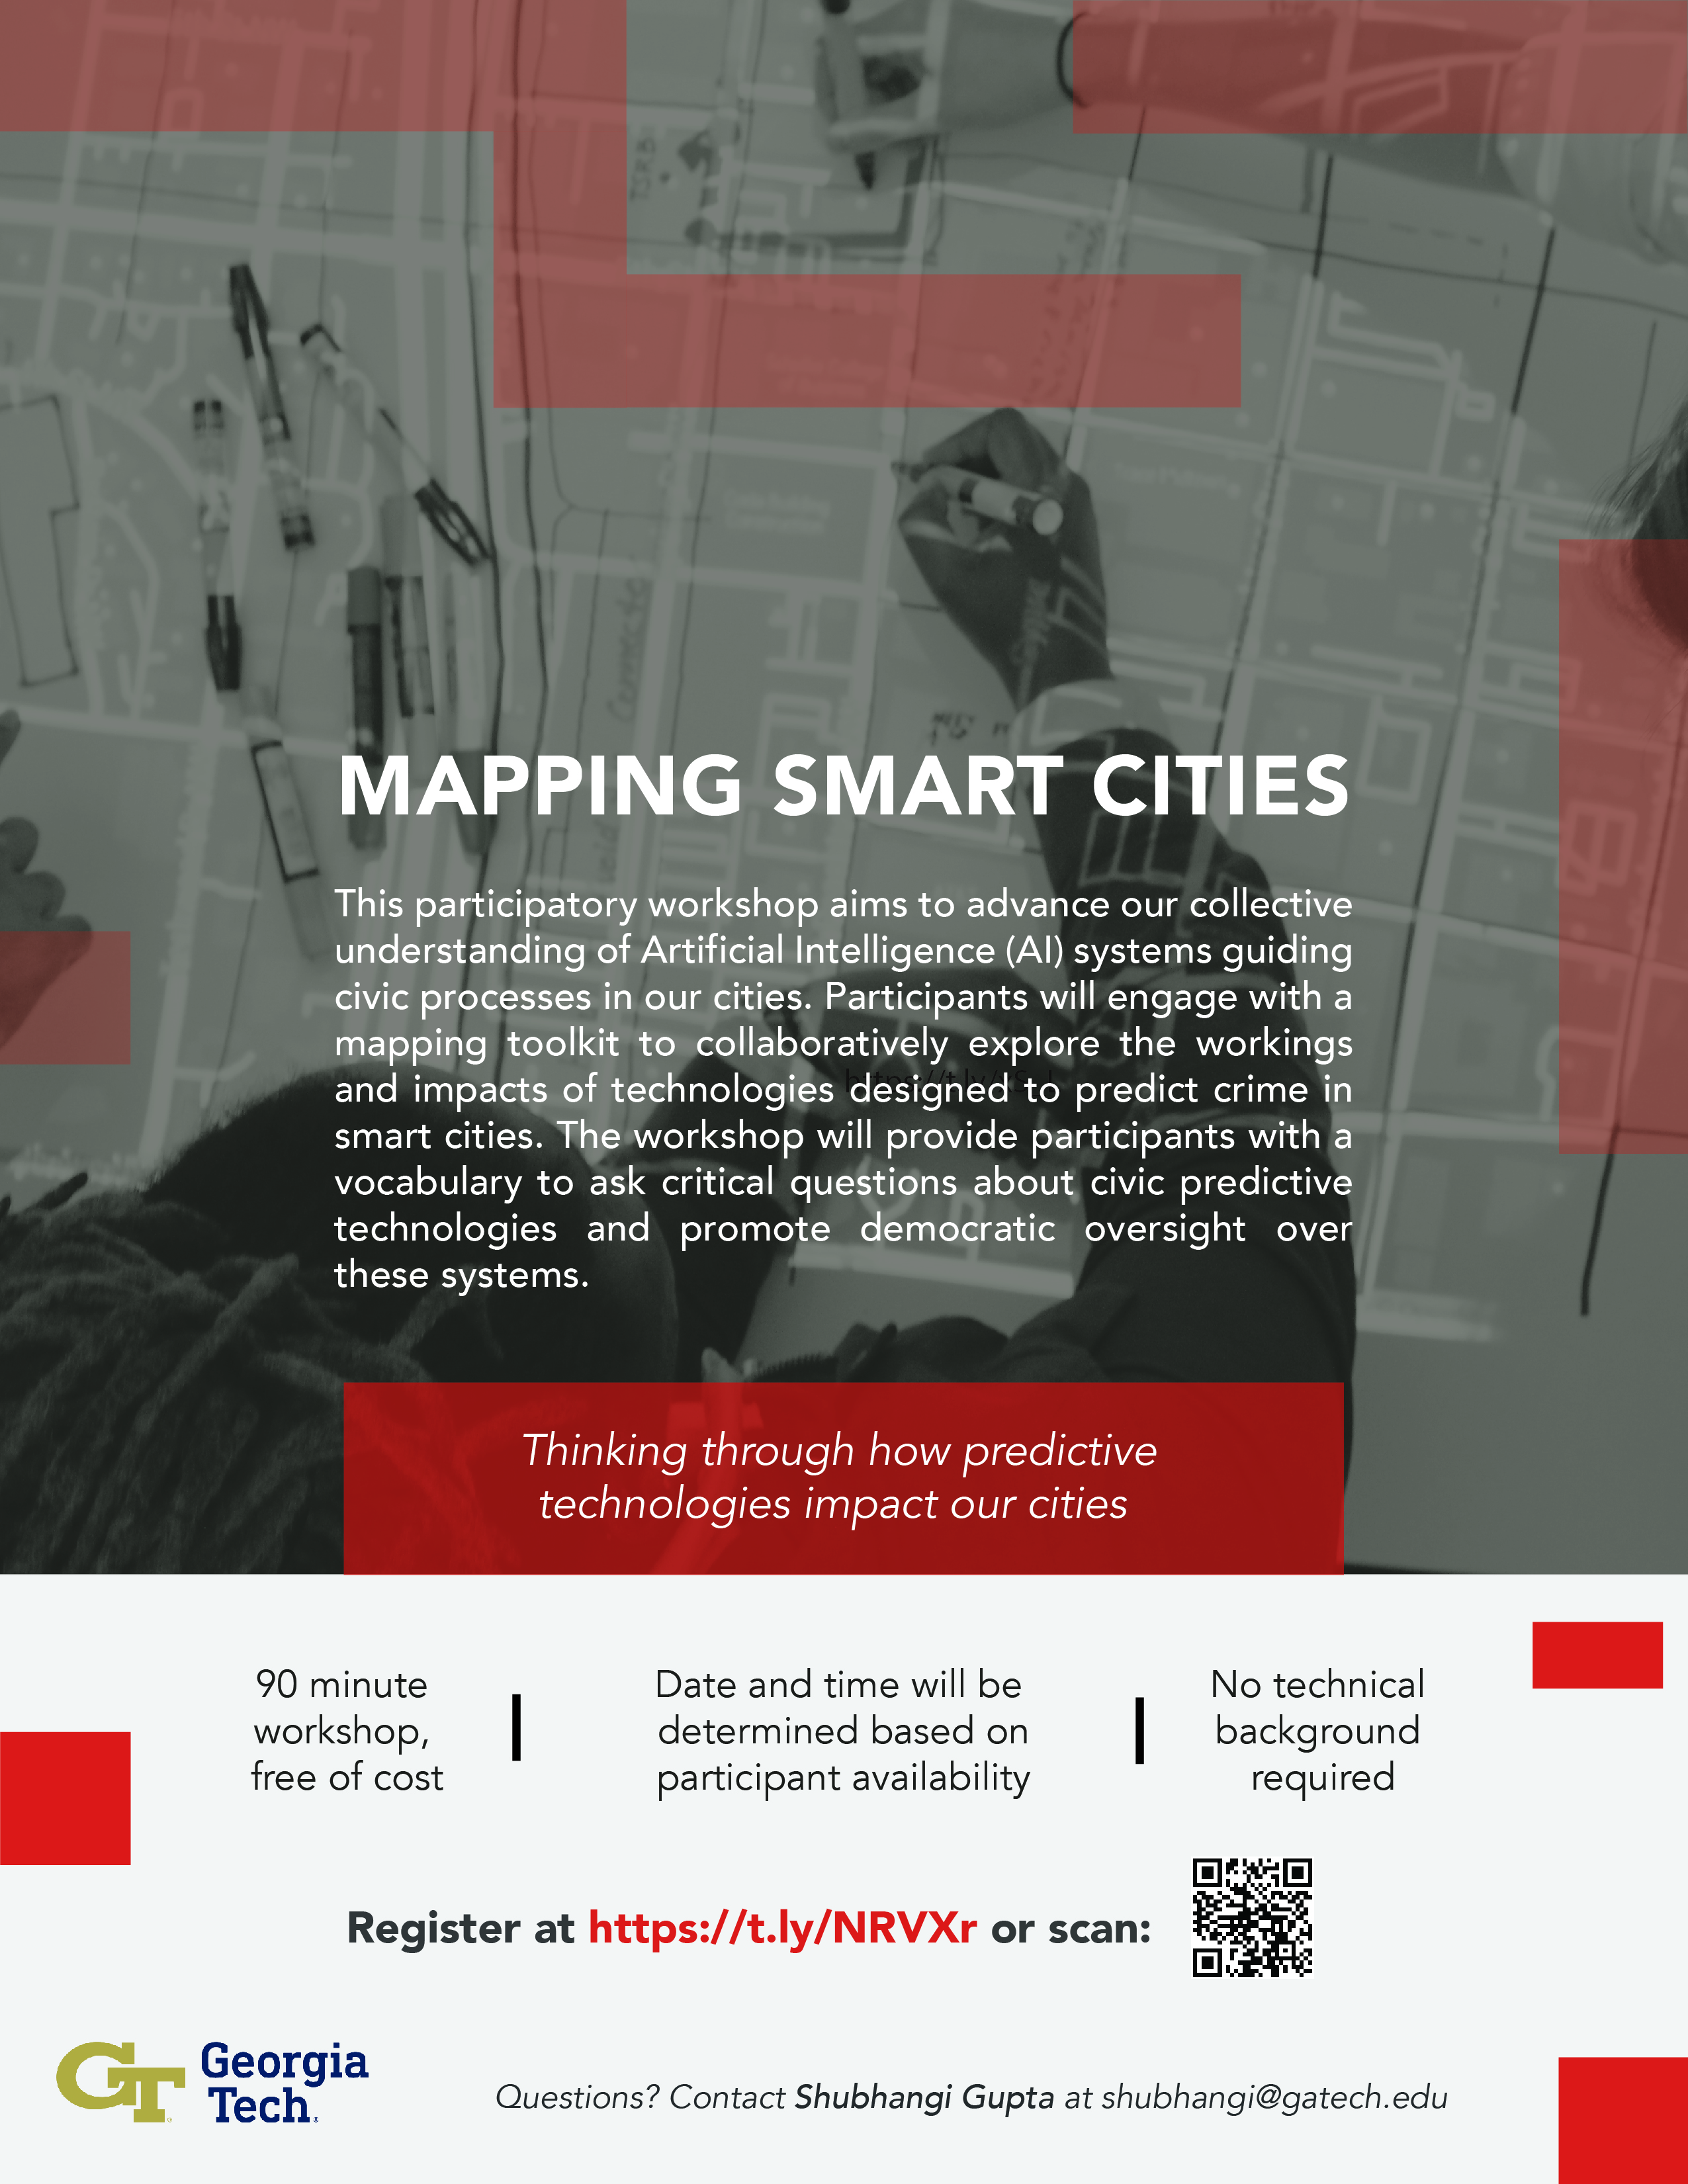
\includegraphics[width=\textwidth]{Appendix/Workshop Materials/flyer_website.jpg}
%     \caption{\todo{Placeholder} Caption}
%     \label{appendix_fig:flyer_website}
% \end{figure}
% \incgraph{Appendix/Workshop Materials/flyer_website.jpg}
\incgraph[documentpaper][height=\paperheight]{Appendix/Workshop Materials/flyer_website.jpg}

% \begin{figure}
%     \centering
%     \includegraphics[width=0.8\textwidth]{Appendix/Workshop Materials/mapping webpage.pdf}
%     \caption{\todo{Placeholder} Caption}
%     \label{appendix_fig:mapping_webpage}
% \end{figure}
\incgraph[documentpaper][height=\paperheight]{Appendix/Workshop Materials/mapping webpage.pdf}

\chapter{Workshop Survey} \label{appB}
Here, I share the survey that was used as a registration form for participation in workshops. 

% \begin{figure}
%     \centering
%     \includegraphics[width=0.5\textwidth]{Appendix/Workshop Materials/Mapping_Civic_AI_Workshop_Survey_Pages/pg1.pdf}
%     \includegraphics[width=0.5\textwidth]{Appendix/Workshop Materials/Mapping_Civic_AI_Workshop_Survey_Pages/pg2.pdf}
%     \includegraphics[width=0.5\textwidth]{Appendix/Workshop Materials/Mapping_Civic_AI_Workshop_Survey_Pages/pg3.pdf}
%     % \caption{\todo{Placeholder} Caption}
%     % \label{appendix_fig:mapping_survey}
% \end{figure}

\incgraph[documentpaper][height=0.8\paperheight]{Appendix/Workshop Materials/Mapping_Civic_AI_Workshop_Survey_Pages/pg1.pdf}
\incgraph[documentpaper][height=0.8\paperheight]{Appendix/Workshop Materials/Mapping_Civic_AI_Workshop_Survey_Pages/pg2.pdf}
\incgraph[documentpaper][height=0.8\paperheight]{Appendix/Workshop Materials/Mapping_Civic_AI_Workshop_Survey_Pages/pg3.pdf}
% \incgraph[documentpaper][height=\paperheight]{Appendix/Workshop Materials/Mapping_Civic_AI_Workshop_Survey.pdf}

\chapter{Workshop Toolkit}
Here I share the toolkit that was developed to guide the workshop interactions and was later shared with the workshop participants. 
% \begin{figure}
%     \centering
%     \includegraphics[width=\textwidth]{Appendix/Workshop Materials/Civic AI toolkit.pdf}
%     \caption{\todo{Placeholder} Caption}
%     \label{appendix_fig:civic_ai_toolkit}
% \end{figure}
% \includepdf{Appendix/Workshop Materials/Civic AI toolkit.pdf}
% \incgraph{Appendix/Workshop Materials/Civic AI toolkit.pdf}
% \incgraph[documentpaper][height=\paperheight]{Appendix/Workshop Materials/Civic AI toolkit.pdf}
\incgraph[documentpaper][height=\paperheight]{Appendix/Workshop Materials/Civic AI toolkit pages/pg1.pdf}

\incgraph[documentpaper][height=\paperheight]{Appendix/Workshop Materials/Civic AI toolkit pages/pg2.pdf}





\end{theappendices}
    \makeBibliography
    % \input{vita}
\end{thesisbody}

\end{document}
